\documentclass[twoside,11pt]{article}

\usepackage{graphicx}
%%\usepackage[draft]{graphicx}

% +
%  Name:
%     sun216.tex
%
%  Purpose:
%     SUN documentation for SURF (SUN/216)
%
%  Authors:
%     Tim Jenness (JACH)
%
%  Copyright:
%     Copyright (C) 1997,1998,1999 Particle Physics and Astronomy
%     Research Council. All Rights Reserved.
%
%  History:
%     1997-1998 (TIMJ)
%        Original versions
%     1998 November 15th (TIMJ)
%        Modify for release 1.3 of SURF
%     1998 December 7th (TIMJ)
%        Add GUARD parameter to REBIN derivatives 
%     1999 November (TIMJ)
%        Add SCUBA2MEM. Update for V1.5
%     {Add further history here}
%
% -


\pagestyle{myheadings}

% -----------------------------------------------------------------------------
% ? Document identification

\newcommand{\scusoft}          {{\sc Surf}}
\newcommand{\micron}           {$\mu$m}   

\newcommand{\stardoccategory}  {Starlink User Note}
\newcommand{\stardocinitials}  {SUN}
\newcommand{\stardocsource}    {sun\stardocnumber}
\newcommand{\stardocnumber}    {216.7}
\newcommand{\stardocauthors}   {T. Jenness, J.~F. Lightfoot\\
                                Joint Astronomy Centre, Hilo, Hawaii}
\newcommand{\stardocdate}      {6 July 2000}
\newcommand{\stardoctitle}     {SURF -- SCUBA User Reduction Facility}
\newcommand{\stardocversion}   {1.6}
\newcommand{\stardocmanual}    {User's manual}
\newcommand{\stardocabstract}  {%
\scusoft\ is a set of ADAM tasks necessary for reducing demodulated 
Submillimetre Common-User Bolometer Array (SCUBA) data obtained from
the James Clerk Maxwell Telescope. The tasks allows one to completely
re-reduce your SCUBA data.

This document describes how to reduce SCUBA data and includes detailed
descriptions of each task.
}
% ? End of document identification

% set up some common package names
\newcommand{\Kappa}{\xref{{\sc{Kappa}}}{sun95}{}}
\newcommand{\Figaro}{\xref{{\sc{Figaro}}}{sun86}{}}
\newcommand{\gaia}{\xref{{\sc{Gaia}}}{sun214}{}}
\newcommand{\convert}{\xref{{\sc{Convert}}}{sun55}{}}
\newcommand{\fluxes}{\xref{{\sc{Fluxes}}}{sun213}{}}
\newcommand{\Iras}{\xref{{\sc{Iras90}}}{sun163}{}}
\newcommand{\ndf}{\xref{NDF}{sun33}{}}
\newcommand{\agi}{\xref{AGI}{sun48}{}}
\newcommand{\ESP}{\xref{ESP}{sun180}{}}
\newcommand{\specx}{\xref{{\sc{Specx}}}{sc8}{}}
\newcommand{\polpack}{\xref{{\sc{Polpack}}}{sun223}{}}
\newcommand{\ccdpack}{\xref{CCDPACK}{sun139}{}}
\newcommand{\cursa}{\xref{{\sc{Cursa}}}{sun190}{}}


% Application tasks
\newcommand{\task}[1]{{\sf #1}}

% ADAM parameters
\newcommand{\param}[1]{{\tt #1}}

% Common tasks
\newcommand{\renoise}{\htmlref{\task{reduce\_noise}}{REDUCE_NOISE}}
\newcommand{\rebin}{\htmlref{\task{rebin}}{REBIN}}
\newcommand{\bolrebin}{\htmlref{\task{bolrebin}}{BOLREBIN}}
\newcommand{\intrebin}{\htmlref{\task{intrebin}}{INTREBIN}}
\newcommand{\calcsky}{\htmlref{\task{calcsky}}{CALCSKY}}
\newcommand{\chgqual}{\htmlref{\task{change\_quality}}{CHANGE_QUALITY}}
\newcommand{\chgflat}{\htmlref{\task{change\_flat}}{CHANGE_FLAT}}
\newcommand{\chgpnt}{\htmlref{\task{change\_pointing}}{CHANGE_POINTING}}
\newcommand{\chgdata}{\htmlref{\task{change\_data}}{CHANGE_DATA}}
\newcommand{\resw}{\htmlref{\task{reduce\_switch}}{REDUCE_SWITCH}}
\newcommand{\flatf}{\htmlref{\task{flatfield}}{FLATFIELD}}
\newcommand{\skydip}{\htmlref{\task{skydip}}{SKYDIP}}
\newcommand{\scuphot}{\htmlref{\task{scuphot}}{SCUPHOT}}
\newcommand{\ext}{\htmlref{\task{extinction}}{EXTINCTION}}
\newcommand{\scuquick}{\htmlref{\task{scuquick}}{SCUQUICK}}
\newcommand{\scuhelp}{\htmlref{\task{scuhelp}}{SCUHELP}}
\newcommand{\remsky}{\htmlref{\task{remsky}}{REMSKY}}
\newcommand{\scuover}{\htmlref{\task{scuover}}{SCUOVER}}
\newcommand{\extdata}{\htmlref{\task{extract\_data}}{EXTRACT_DATA}}
\newcommand{\sculog}{\htmlref{\task{sculog}}{SCULOG}}
\newcommand{\scucat}{\htmlref{\task{scucat}}{SCUCAT}}
\newcommand{\photsum}{\htmlref{\task{photsum}}{PHOTSUM}}
\newcommand{\mapsum}{\htmlref{\task{mapsum}}{MAPSUM}}
\newcommand{\skysum}{\htmlref{\task{skysum}}{SKYSUM}}
\newcommand{\pointsum}{\htmlref{\task{pointsum}}{POINTSUM}}
\newcommand{\qdraw}{\htmlref{\task{qdraw}}{QDRAW}}
\newcommand{\sigclip}{\htmlref{\task{sigclip}}{SIGCLIP}}
\newcommand{\restore}{\htmlref{\task{restore}}{RESTORE}}
\newcommand{\sdip}{\htmlref{\task{sdip}}{SDIP}}
\newcommand{\scupa}{\htmlref{\task{scupa}}{SCUPA}}
\newcommand{\obssum}{\htmlref{\task{obssum}}{OBSSUM}}
\newcommand{\despike}{\htmlref{\task{despike}}{DESPIKE}}
\newcommand{\despikeb}{\htmlref{\task{despike2}}{DESPIKE2}}
\newcommand{\extflat}{\htmlref{\task{extract\_flat}}{EXTRACT_FLAT}}
\newcommand{\scushift}{\htmlref{\task{scushift}}{SCUSHIFT}}
\newcommand{\scuclip}{\htmlref{\task{scuclip}}{SCUCLIP}}
\newcommand{\scuclkerr}{\htmlref{\task{scuclkerr}}{SCUCLKERR}}
\newcommand{\scanrlb}{\htmlref{\task{scan\_rlb}}{SCAN_RLB}}
\newcommand{\dspbol}{\htmlref{\task{dspbol}}{DSPBOL}}
\newcommand{\pltbol}{\htmlref{\task{pltbol}}{PLTBOL}}
\newcommand{\rlinplot}{\htmlref{\task{rlinplot}}{RLINPLOT}}
\newcommand{\scuplot}{\htmlref{\task{scuplot}}{SCUPLOT}}
\newcommand{\remdbm}{\htmlref{\task{remdbm}}{REMDBM}}
\newcommand{\scumakewt}{\htmlref{\task{scumakewt}}{SCUMAKEWT}}
\newcommand{\chgnacent}{\htmlref{\task{change\_nacentre}}{CHANGE_NACENTRE}}
\newcommand{\scunoise}{\htmlref{\task{scunoise}}{SCUNOISE}}
\newcommand{\setbolwt}{\htmlref{\task{setbolwt}}{SETBOLWT}}
\newcommand{\adddbm}{\htmlref{\task{add\_dbm}}{ADD_DBM}}
\newcommand{\remip}{\htmlref{\task{remip}}{REMIP}}
\newcommand{\scusetenv}{\htmlref{\task{scusetenv}}{SCUSETENV}}
\newcommand{\scubamem}{\htmlref{\task{scuba2mem}}{SCUBA2MEM}}


% Non surf tasks

\newcommand{\fillbad}{\xref{\task{fillbad}}{sun95}{FILLBAD}}
\newcommand{\ndftrace}{\xref{\task{ndftrace}}{sun95}{NDFTRACE}}
\newcommand{\glitch}{\xref{\task{glitch}}{sun95}{GLITCH}}
\newcommand{\display}{\xref{\task{display}}{sun95}{DISPLAY}}
\newcommand{\linplot}{\xref{\task{linplot}}{sun95}{LINPLOT}}
\newcommand{\mlinplot}{\xref{\task{mlinplot}}{sun95}{MLINPLOT}}
\newcommand{\drawsig}{\xref{\task{drawsig}}{sun95}{DRAWSIG}}
\newcommand{\centroid}{\xref{\task{centroid}}{sun95}{CENTROID}}
\newcommand{\setaxis}{\xref{\task{setaxis}}{sun95}{SETAXIS}}
\newcommand{\kstest}{\xref{\task{kstest}}{sun95}{KSTEST}}
\newcommand{\stats}{\xref{\task{stats}}{sun95}{STATS}}
\newcommand{\thresh}{\xref{\task{thresh}}{sun95}{THRESH}}
\newcommand{\setbb}{\xref{\task{setbb}}{sun95}{SETBB}}
\newcommand{\fitslist}{\xref{\task{fitslist}}{sun95}{FITSLIST}}
\newcommand{\fourier}{\xref{\task{fourier}}{sun95}{FOURIER}}
\newcommand{\hislist}{\xref{\task{hislist}}{sun95}{HISLIST}}
\newcommand{\ndffits}{\xref{\task{ndf2fits}}{sun55}{NDF2FITS}}
\newcommand{\ndftoascii}{\xref{\task{ndf2ascii}}{sun55}{NDF2ASCII}}
\newcommand{\cadd}{\xref{\task{cadd}}{sun95}{CADD}}
\newcommand{\hdstrace}{\xref{\task{hdstrace}}{sun102}{}}
\newcommand{\psmerge}{\xref{\task{psmerge}}{sun164}{}}
\newcommand{\wdfits}{\xref{\task{wdfits}}{sun86}{WDFITS}}
\newcommand{\delobj}{\xref{\task{delobj}}{sun86}{DELOBJ}}
\newcommand{\sclean}{\xref{\task{sclean}}{sun86}{SCLEAN}}
\newcommand{\setvar}{\xref{\task{setvar}}{sun95}{SETVAR}}
\newcommand{\wcsalign}{\xref{\task{wcsalign}}{sun95}{WCSALIGN}}
\newcommand{\ndfcopy}{\xref{\task{ndfcopy}}{sun95}{NDFCOPY}}
\newcommand{\manic}{\xref{\task{manic}}{sun95}{MANIC}}
\newcommand{\cdiv}{\xref{\task{cdiv}}{sun95}{CDIV}}
\newcommand{\sub}{\xref{\task{sub}}{sun95}{SUB}}
\newcommand{\cursor}{\xref{\task{cursor}}{sun95}{CURSOR}}
\newcommand{\gdset}{\xref{\task{gdset}}{sun95}{GDSET}}
\newcommand{\image}{\xref{\task{image}}{sun86}{IMAGE}}
\newcommand{\gaufit}{\xref{\task{gaufit}}{sun180}{GAUFIT}}
\newcommand{\makemos}{\xref{\task{makemos}}{sun139}{MAKEMOS}}

\newcommand{\polimp}{\xref{\task{polimp}}{sun223}{POLIMP}}
\newcommand{\polcal}{\xref{\task{polcal}}{sun223}{POLCAL}}
\newcommand{\polbin}{\xref{\task{polbin}}{sun223}{POLBIN}}
\newcommand{\polvec}{\xref{\task{polvec}}{sun223}{POLVEC}}
\newcommand{\polplot}{\xref{\task{polplot}}{sun223}{POLPLOT}}
\newcommand{\polstack}{\xref{\task{polstack}}{sun223}{POLSTACK}}

\newcommand{\catselect}{\xref{\task{catselect}}{sun190}{}}


%%% Some macros

% quick routine description. Now uses a description list

% This is the latex version

\newcommand{\quickdes}[3]{
\item \textbf{#1:} {\raggedright  #2 (page \pageref{#3})}}

% The HTML version is redefined later when the htmlonly environment
% is defined

% Environment for indenting and using a small font.
\newenvironment{myquote}{\begin{quote}\begin{small}}{\end{small}\end{quote}}

\newcommand{\text}[1]{{\small \tt #1}}


% +
%  Name:
%     sun.tex
%
%  Purpose:
%     Template for Starlink User Note (SUN) documents.
%     Refer to SUN/199
%
%  Authors:
%     AJC: A.J.Chipperfield (Starlink, RAL)
%     BLY: M.J.Bly (Starlink, RAL)
%     PWD: Peter W. Draper (Starlink, Durham University)
%
%  History:
%     17-JAN-1996 (AJC):
%        Original with hypertext macros, based on MDL plain originals.
%     16-JUN-1997 (BLY):
%        Adapted for LaTeX2e.
%        Added picture commands.
%     13-AUG-1998 (PWD):
%        Converted for use with LaTeX2HTML version 98.2 and
%        Star2HTML version 1.3.
%     {Add further history here}
%
% -

\newcommand{\stardocname}{\stardocinitials /\stardocnumber}
\markboth{\stardocname}{\stardocname}
\setlength{\textwidth}{160mm}
\setlength{\textheight}{230mm}
\setlength{\topmargin}{-2mm}
\setlength{\oddsidemargin}{0mm}
\setlength{\evensidemargin}{0mm}
\setlength{\parindent}{0mm}
\setlength{\parskip}{\medskipamount}
\setlength{\unitlength}{1mm}

% -----------------------------------------------------------------------------
%  Hypertext definitions.
%  ======================
%  These are used by the LaTeX2HTML translator in conjunction with star2html.

%  Comment.sty: version 2.0, 19 June 1992
%  Selectively in/exclude pieces of text.
%
%  Author
%    Victor Eijkhout                                      <eijkhout@cs.utk.edu>
%    Department of Computer Science
%    University Tennessee at Knoxville
%    104 Ayres Hall
%    Knoxville, TN 37996
%    USA

%  Do not remove the %begin{latexonly} and %end{latexonly} lines (used by 
%  LaTeX2HTML to signify text it shouldn't process).
%begin{latexonly}
\makeatletter
\def\makeinnocent#1{\catcode`#1=12 }
\def\csarg#1#2{\expandafter#1\csname#2\endcsname}

\def\ThrowAwayComment#1{\begingroup
    \def\CurrentComment{#1}%
    \let\do\makeinnocent \dospecials
    \makeinnocent\^^L% and whatever other special cases
    \endlinechar`\^^M \catcode`\^^M=12 \xComment}
{\catcode`\^^M=12 \endlinechar=-1 %
 \gdef\xComment#1^^M{\def\test{#1}
      \csarg\ifx{PlainEnd\CurrentComment Test}\test
          \let\html@next\endgroup
      \else \csarg\ifx{LaLaEnd\CurrentComment Test}\test
            \edef\html@next{\endgroup\noexpand\end{\CurrentComment}}
      \else \let\html@next\xComment
      \fi \fi \html@next}
}
\makeatother

\def\includecomment
 #1{\expandafter\def\csname#1\endcsname{}%
    \expandafter\def\csname end#1\endcsname{}}
\def\excludecomment
 #1{\expandafter\def\csname#1\endcsname{\ThrowAwayComment{#1}}%
    {\escapechar=-1\relax
     \csarg\xdef{PlainEnd#1Test}{\string\\end#1}%
     \csarg\xdef{LaLaEnd#1Test}{\string\\end\string\{#1\string\}}%
    }}

%  Define environments that ignore their contents.
\excludecomment{comment}
\excludecomment{rawhtml}
\excludecomment{htmlonly}

%  Hypertext commands etc. This is a condensed version of the html.sty
%  file supplied with LaTeX2HTML by: Nikos Drakos <nikos@cbl.leeds.ac.uk> &
%  Jelle van Zeijl <jvzeijl@isou17.estec.esa.nl>. The LaTeX2HTML documentation
%  should be consulted about all commands (and the environments defined above)
%  except \xref and \xlabel which are Starlink specific.

\newcommand{\htmladdnormallinkfoot}[2]{#1\footnote{#2}}
\newcommand{\htmladdnormallink}[2]{#1}
\newcommand{\htmladdimg}[1]{}
\newcommand{\hyperref}[4]{#2\ref{#4}#3}
\newcommand{\htmlref}[2]{#1}
\newcommand{\htmlimage}[1]{}
\newcommand{\htmladdtonavigation}[1]{}

\newenvironment{latexonly}{}{}
\newcommand{\latex}[1]{#1}
\newcommand{\html}[1]{}
\newcommand{\latexhtml}[2]{#1}
\newcommand{\HTMLcode}[2][]{}

%  Starlink cross-references and labels.
\newcommand{\xref}[3]{#1}
\newcommand{\xlabel}[1]{}

%  LaTeX2HTML symbol.
\newcommand{\latextohtml}{\LaTeX2\texttt{HTML}}

%  Define command to re-centre underscore for Latex and leave as normal
%  for HTML (severe problems with \_ in tabbing environments and \_\_
%  generally otherwise).
\renewcommand{\_}{\texttt{\symbol{95}}}




% -----------------------------------------------------------------------------
%  Debugging.
%  =========
%  Remove % on the following to debug links in the HTML version using Latex.

% \newcommand{\hotlink}[2]{\fbox{\begin{tabular}[t]{@{}c@{}}#1\\\hline{\footnotesize #2}\end{tabular}}}
% \renewcommand{\htmladdnormallinkfoot}[2]{\hotlink{#1}{#2}}
% \renewcommand{\htmladdnormallink}[2]{\hotlink{#1}{#2}}
% \renewcommand{\hyperref}[4]{\hotlink{#1}{\S\ref{#4}}}
% \renewcommand{\htmlref}[2]{\hotlink{#1}{\S\ref{#2}}}
% \renewcommand{\xref}[3]{\hotlink{#1}{#2 -- #3}}
%end{latexonly}
% -----------------------------------------------------------------------------
% ? Document specific \newcommand or \newenvironment commands.

%+
%  Name:
%     SST.TEX

%  Purpose:
%     Define LaTeX commands for laying out Starlink routine descriptions.

%  Language:
%     LaTeX

%  Type of Module:
%     LaTeX data file.

%  Description:
%     This file defines LaTeX commands which allow routine documentation
%     produced by the SST application PROLAT to be processed by LaTeX and
%     by LaTeX2html. The contents of this file should be included in the
%     source prior to any statements that make of the sst commnds.

%  Notes:
%     The style file html.sty provided with LaTeX2html needs to be used.
%     This must be before this file.

%  Authors:
%     RFWS: R.F. Warren-Smith (STARLINK)
%     PDRAPER: P.W. Draper (Starlink - Durham University)

%  History:
%     10-SEP-1990 (RFWS):
%        Original version.
%     10-SEP-1990 (RFWS):
%        Added the implementation status section.
%     12-SEP-1990 (RFWS):
%        Added support for the usage section and adjusted various spacings.
%     8-DEC-1994 (PDRAPER):
%        Added support for simplified formatting using LaTeX2html.
%     {enter_further_changes_here}

%  Bugs:
%     {note_any_bugs_here}

%-

%  Define length variables.
\newlength{\sstbannerlength}
\newlength{\sstcaptionlength}
\newlength{\sstexampleslength}
\newlength{\sstexampleswidth}

%  Define a \tt font of the required size.
\latex{\newfont{\ssttt}{cmtt10 scaled 1095}}
\html{\newcommand{\ssttt}{\tt}}

%  Define a command to produce a routine header, including its name,
%  a purpose description and the rest of the routine's documentation.
\newcommand{\sstroutine}[3]{
   \goodbreak
   \rule{\textwidth}{0.5mm}
   \vspace{-7ex}
   \newline
   \settowidth{\sstbannerlength}{{\Large {\bf #1}}}
   \setlength{\sstcaptionlength}{\textwidth}
   \setlength{\sstexampleslength}{\textwidth}
   \addtolength{\sstbannerlength}{0.5em}
   \addtolength{\sstcaptionlength}{-2.0\sstbannerlength}
   \addtolength{\sstcaptionlength}{-5.0pt}
   \settowidth{\sstexampleswidth}{{\bf Examples:}}
   \addtolength{\sstexampleslength}{-\sstexampleswidth}
   \parbox[t]{\sstbannerlength}{\flushleft{\Large {\bf #1}}}
   \parbox[t]{\sstcaptionlength}{\center{\Large #2}}
   \parbox[t]{\sstbannerlength}{\flushright{\Large {\bf #1}}}
   \begin{description}
      #3
   \end{description}
}

%  Format the description section.
\newcommand{\sstdescription}[1]{\item[Description:] #1}

%  Format the usage section.
\newcommand{\sstusage}[1]{\item[Usage:] \mbox{}
\\[1.3ex]{\raggedright \ssttt #1}}

%  Format the invocation section.
\newcommand{\sstinvocation}[1]{\item[Invocation:]\hspace{0.4em}{\tt #1}}

%  Format the arguments section.
\newcommand{\sstarguments}[1]{
   \item[Arguments:] \mbox{} \\
   \vspace{-3.5ex}
   \begin{description}
      #1
   \end{description}
}

%  Format the returned value section (for a function).
\newcommand{\sstreturnedvalue}[1]{
   \item[Returned Value:] \mbox{} \\
   \vspace{-3.5ex}
   \begin{description}
      #1
   \end{description}
}

%  Format the parameters section (for an application).
\newcommand{\sstparameters}[1]{
   \item[Parameters:] \mbox{} \\
   \vspace{-3.5ex}
   \begin{description}
      #1
   \end{description}
}

%  Format the examples section.
\newcommand{\sstexamples}[1]{
   \item[Examples:] \mbox{} \\
   \vspace{-3.5ex}
   \begin{description}
      #1
   \end{description}
}

%  Define the format of a subsection in a normal section.
\newcommand{\sstsubsection}[1]{ \item[{#1}] \mbox{} \\}

%  Define the format of a subsection in the examples section.
\newcommand{\sstexamplesubsection}[2]{\sloppy
\item[\parbox{\sstexampleslength}{\ssttt #1}] \mbox{} \vspace{1.0ex}
\\ #2 }

%  Format the notes section.
\newcommand{\sstnotes}[1]{\item[Notes:] \mbox{} \\[1.3ex] #1}

%  Provide a general-purpose format for additional (DIY) sections.
\newcommand{\sstdiytopic}[2]{\item[{\hspace{-0.35em}#1\hspace{-0.35em}:}]
\mbox{} \\[1.3ex] #2}

%  Format the implementation status section.
\newcommand{\sstimplementationstatus}[1]{
   \item[{Implementation Status:}] \mbox{} \\[1.3ex] #1}

%  Format the bugs section.
\newcommand{\sstbugs}[1]{\item[Bugs:] #1}

%  Format a list of items while in paragraph mode.
\newcommand{\sstitemlist}[1]{
  \mbox{} \\
  \vspace{-3.5ex}
  \begin{itemize}
     #1
  \end{itemize}
}

%  Define the format of an item.
\newcommand{\sstitem}{\item}

%% Now define html equivalents of those already set. These are used by
%  latex2html and are defined in the html.sty files.
\begin{htmlonly}

%  sstroutine.
   \newcommand{\sstroutine}[3]{
      \subsection{#1\xlabel{#1}-\label{#1}#2}
      \begin{description}
         #3
      \end{description}
   }

%  sstdescription
   \newcommand{\sstdescription}[1]{\item[Description:]
      \begin{description}
         #1
      \end{description}
      \\
   }

%  sstusage
   \newcommand{\sstusage}[1]{\item[Usage:]
      \begin{description}
         {\ssttt #1}
      \end{description}
      \\
   }

%  sstinvocation
   \newcommand{\sstinvocation}[1]{\item[Invocation:]
      \begin{description}
         {\ssttt #1}
      \end{description}
      \\
   }

%  sstarguments
   \newcommand{\sstarguments}[1]{
      \item[Arguments:] \\
      \begin{description}
         #1
      \end{description}
      \\
   }

%  sstreturnedvalue
   \newcommand{\sstreturnedvalue}[1]{
      \item[Returned Value:] \\
      \begin{description}
         #1
      \end{description}
      \\
   }

%  sstparameters
   \newcommand{\sstparameters}[1]{
      \item[Parameters:] \\
      \begin{description}
         #1
      \end{description}
      \\
   }

%  sstexamples
   \newcommand{\sstexamples}[1]{
      \item[Examples:] \\
      \begin{description}
         #1
      \end{description}
      \\
   }

%  sstsubsection
   \newcommand{\sstsubsection}[1]{\item[{#1}]}

%  sstexamplesubsection
   \newcommand{\sstexamplesubsection}[2]{\item[{\ssttt #1}] #2}

%  sstnotes
   \newcommand{\sstnotes}[1]{\item[Notes:] #1 }

%  sstdiytopic
   \newcommand{\sstdiytopic}[2]{\item[{#1}] #2 }

%  sstimplementationstatus
   \newcommand{\sstimplementationstatus}[1]{
      \item[Implementation Status:] #1
   }

%  sstitemlist
   \newcommand{\sstitemlist}[1]{
      \begin{itemize}
         #1
      \end{itemize}
      \\
   }
%  sstitem
   \newcommand{\sstitem}{\item}

\end{htmlonly}

%  End of "sst.tex" layout definitions.
%.




% ? End of document specific commands
% -----------------------------------------------------------------------------
%  Title Page.
%  ===========
\renewcommand{\thepage}{\roman{page}}
\begin{document}
\thispagestyle{empty}



%  Latex document header.
%  ======================
\begin{latexonly}
   CCLRC / {\textsc Rutherford Appleton Laboratory} \hfill {\textbf \stardocname}\\
   {\large Particle Physics \& Astronomy Research Council}\\
   {\large Starlink Project\\}
   {\large \stardoccategory\ \stardocnumber}
   \begin{flushright}
   \stardocauthors\\
   \stardocdate
   \end{flushright}
   \vspace{-4mm}
   \rule{\textwidth}{0.5mm}
   \vspace{5mm}
   \begin{center}
   
\includegraphics[width=2.0in]{sun216_logo.eps}

   {\Huge\textbf  \stardoctitle \\ [2.5ex]}
   {\LARGE\textbf \stardocversion \\ [4ex]}
   {\Huge\textbf  \stardocmanual}
   \end{center}
   \vspace{5mm}

% ? Add picture here if required for the LaTeX version.
%   e.g. \includegraphics[scale=0.3]{filename.ps}
% ? End of picture

% ? Heading for abstract if used.
   \vspace{10mm}
   \begin{center}
      {\Large\textbf Abstract}
   \end{center}
% ? End of heading for abstract.
\end{latexonly}

%  HTML documentation header.
%  ==========================
\begin{htmlonly}
   \xlabel{}
   \begin{rawhtml} <H1 ALIGN=CENTER> \end{rawhtml}
      \stardoctitle\\
      \stardocversion\\
      \stardocmanual
   \begin{rawhtml} </H1> <HR> \end{rawhtml}

% ? Add picture here if required for the hypertext version.
%   e.g. \includegraphics[scale=0.7]{filename.ps}

\includegraphics[width=2.0in]{sun216_logo.eps}
% ? End of picture

   \begin{rawhtml} <P> <I> \end{rawhtml}
   \stardoccategory\ \stardocnumber \\
   \stardocauthors \\
   \stardocdate
   \begin{rawhtml} </I> </P> <H3> \end{rawhtml}
      \htmladdnormallink{CCLRC}{http://www.cclrc.ac.uk} /
      \htmladdnormallink{Rutherford Appleton Laboratory}
                        {http://www.cclrc.ac.uk/ral} \\
      \htmladdnormallink{Particle Physics \& Astronomy Research Council}
                        {http://www.pparc.ac.uk} \\
   \begin{rawhtml} </H3> <H2> \end{rawhtml}
      \htmladdnormallink{Starlink Project}{http://star-www.rl.ac.uk/}
   \begin{rawhtml} </H2> \end{rawhtml}
   \htmladdnormallink{\htmladdimg{source.gif} Retrieve hardcopy}
      {http://star-www.rl.ac.uk/cgi-bin/hcserver?\stardocsource}\\

%  HTML document table of contents. 
%  ================================
%  Add table of contents header and a navigation button to return to this 
%  point in the document (this should always go before the abstract \section). 
  \label{stardoccontents}
  \begin{rawhtml} 
    <HR>
    <H2>Contents</H2>
  \end{rawhtml}
  \htmladdtonavigation{\htmlref{\htmladdimg{contents_motif.gif}}
        {stardoccontents}}

% ? New section for abstract if used.

  \section{\xlabel{abstract} Abstract }

% ? End of new section for abstract
\end{htmlonly}

% -----------------------------------------------------------------------------
% ? Document Abstract. (if used)
%  ==================

\stardocabstract

% ? End of document abstract
% -----------------------------------------------------------------------------
% ? Latex document Table of Contents (if used).
%  ===========================================
  \newpage
  \begin{latexonly}
    \setlength{\parskip}{0mm}
    \tableofcontents
    \setlength{\parskip}{\medskipamount}
    \markboth{\stardocname}{\stardocname}
  \end{latexonly}
% ? End of Latex document table of contents
% -----------------------------------------------------------------------------
\cleardoublepage
\renewcommand{\thepage}{\arabic{page}}
\setcounter{page}{1}


\section{\xlabel{introduction}Introduction\label{introduction}}

The Submillimetre Common-User Bolometer Array (SCUBA) \cite{spiewsh,mnscu} is
a continuum instrument on the \htmladdnormallinkfoot{James Clerk Maxwell
Telescope}{http://www.jach.hawaii.edu/JACpublic/JCMT/}, Mauna Kea, Hawaii.
SCUBA has two arrays and can observe simultaneously at two wavelengths (three
wavelengths when using the photometry pixels) -- the layout of the SCUBA
arrays is shown in Fig.\ \ref{arrays}.

The on-line system produces data in the Starlink \ndf\ format \cite{ndf}.
Both the raw demodulated data (signified by `\_dem\_' in the file name) and a
reduced image (`RO' file) can be stored.  This package is designed to take the
demodulated data (stored in the \texttt{[.dem]} directory on-line) and remove SCUBA
dependent effects. In the case of MAP data, a rectangular-gridded image is
produced, for PHOTOM observations a set of photometry data. Packages such as
\gaia \cite{gaia} or \Kappa\cite{kappa} \display, for MAP, and \Kappa\
\linplot\ and \drawsig, for PHOTOM, can be used for further
processing. Calibration via planet observations can be determined using the
\fluxes \cite{fluxes} package.  The \convert \cite{convert} package can
also be used to export the data into your favoured data format.

The RO file (signified by `\_red\_' in the file name) contains the reduced
data (image, skydip result, photometry result) calculated by the on-line
system. These data can be examined either by using \hdstrace\cite{hdstrace} or, for images, a Starlink-compatible image display
package (note that nested NDFs are used - see Appendix \ref{filenames}).

\begin{latexonly}
\begin{center}
\begin{figure}
\hspace*{20mm}
\includegraphics[width=0.90\textheight,angle=90]{sun216_arrays.eps}
\caption{The SCUBA arrays}
\label{arrays}
\end{figure}
\end{center}
\end{latexonly}

\begin{htmlonly}
\begin{figure}
%%\htmlimage{scale=0.65}
%%\epsfig{file=sun216_arrays.eps,angle=90,width=3.0in,clip=}
\includegraphics[scale=0.65]{sun216_arrays.eps}
\caption{The SCUBA arrays.}
\label{arrays}
\end{figure}

\end{htmlonly}

\section{\xlabel{startup}Starting up \scusoft \label{startup}}

The \scusoft\ environment can be initialised from the C-shell using the
\texttt{surf} command.

\begin{myquote}
\begin{verbatim}
% surf
 
   SURF - SCUBA User Reduction Facility
     Commands are now available -- (Version 1.4-0)
 
     Type scuhelp for help on SURF commands.
     Type "showme sun216" to browse the hypertext documentation.

\end{verbatim}
\end{myquote}

Note that the \texttt{\%} represents the C-shell prompt and shouldn't be typed.
\scusoft\ is also available from the ICL command language.


\subsection{Getting help}

Help is available in two forms; from the command-line and via a hypertext 
version of this document. The command-line version is available with

\begin{myquote}
\begin{verbatim}
% scuhelp
\end{verbatim}
\end{myquote}

and the hypertext version can be obtained with

\begin{myquote}
\begin{verbatim}
% findme surf
\end{verbatim}
\end{myquote}
or
\begin{myquote}
\begin{verbatim}
% showme sun216
\end{verbatim}
\end{myquote}
A WWW browser will be started up if necessary.

It is possible to start the help system when responding to
an ADAM prompt. Supplying a `?' will give more information on the
parameter being requested and supplying `??' will start the interactive
help system.

There are also two cookbooks available; one dealing with the reduction of
photometry data \cite{S97} and the other dealing with the reduction of
map data \cite{SANDELL97}.

Alternatively the JCMT software group can be contacted directly via the
\htmladdnormallinkfoot{World-Wide-Web}{http://www.jach.hawaii.edu/JACpublic/JCMT/software}.
Information on known bugs and updates will be available there.

A mailing list now exists for discussing SCUBA data reduction techniques.  The
list is at
\htmladdnormallink{\texttt{scubadr@jach.hawaii.edu}}{mailto:scubadr@jach.hawaii.edu}. To
subscribe, send an email message to
\htmladdnormallink{\texttt{majordomo@jach.hawaii.edu}}{mailto:majordomo@jach.hawaii.edu}
with an empty subject and containing the message:
\begin{myquote}
\begin{verbatim}
subscribe scubadr you@some.email.address
\end{verbatim}
\end{myquote}


\section{\xlabel{journal}What data do I have?\label{journal}}

Journal software is available to aid with book-keeping of observation
files.\footnote{only available if {\tt ndfperl} is installed on your system
(see Appendix \ref{ndfperl})}  If you are reducing your data at the Joint
Astronomy Centre you may need to read Appendix \ref{JAC} to find where the
data are stored.

\sculog\ will give a summary of all NDF files in
a directory (the directory is the current working directory and, if set, the
directory specified by the {\sc datadir} environment variable (\S\ref{env})).
\begin{myquote}
\begin{verbatim}
% sculog
 
 Enter starting observation number [0] 94
 Enter final observation number [last] 95
-Log for directory: /jcmt_sw/scuba/sun216
                    /scuba/observe/apr25/dem
94      JUPITER             PHOTOM        1997:4:25     17:43:39.99893
   RA: 21 26  1.54 Dec: -15 42 52.0 (J2000) Observed centre: PLANET
   Mean airmass: 1.2310825  Bolometers:   H7                Filter: 450N:850
   Throw:    60 arcsec  AZ  Integrations: 4      Measurements: 1
   Accept: not used         DATA_KPT: DEMOD              Gain: 1
   Observation file: jupiter_h7.obs             Data file: apr25_dem_0094
 
---------
 
95                 SKYDIP        1997:4:25     17:46:26.99799
   Bolometers:   SHORT_DC,LONG_DC                Filter: 450N:850
   Max EL: 80   Min EL: 15  Integrations: 20     Measurements: 10
   Accept: NO               DATA_KPT: DEMOD              Gain: 1
   Observation file: scuba_skydip.obs           Data file: apr25_dem_0095
---------
\end{verbatim}
\end{myquote}
In most cases \sculog\ provides far too much information and a one 
line summary is more desirable. \obssum\footnote{\obssum\ is simply an alias
for \texttt{\sculog\ $-$summary}.} is provided for this purpose:
\begin{myquote}
\begin{verbatim}
% obssum -demod
 
 Enter starting observation number [0] 92
 Enter final observation number [last] 98
-Log for directory: /jcmt_sw/scuba/sun216
                    /scuba/observe/apr25/dem
 
 #    HST    Obsmode   Source   Meas/Int Airmass  Filter  Bolometers
---- -----   --------- -------  -------- ------- -------- ----------
92   07:33   PHOTOM    JUPITER     1/4   1.229 450N:850N G4
93   07:36   PHOTOM    JUPITER     1/4   1.229 450N:850N G3
94   07:43   PHOTOM    JUPITER     1/4   1.231 450N:850N H7
95   07:46   SKYDIP    SKY        10/20        450N:850N SHORT_DC,LONG_DC
96   07:54   POINTING  uranus      1/2   1.337 450N:850N LONG
97   07:57   MAP       uranus      1/1   1.407 450N:850N SHORT,LONG
98   08:45   POINTING  uranus      1/2   1.488 450N:850N LONG
\end{verbatim}
\end{myquote}
In this example a summary listing has been requested for observations 92
through 98 from the {\sc \$datadir} directory %%%% $ for emacs 
(there were no
demodulated data files in my current directory).  The `--demod' flag indicated
that I am only interested in raw demodulated data (i.e.\ files containing
`\_dem\_' in their names). \sculog\ (and \obssum) supports many more options
and these are detailed in \S\ref{surf:sculog}.

Alternatively, listings of certain observations can be obtained by using the
more specialized listing programs \photsum, \mapsum, \pointsum\ and
\skysum. \pointsum\ lists pointing observations, \photsum\ lists photometry
observations (and, in fact, skydip observations), \mapsum\ lists map
observations and \skysum\ lists skydip observations. Using
\photsum\ instead of \sculog\ on the data used above gives:
\begin{myquote}
\begin{verbatim}
% photsum --begin=92 --end=98
 #    HST    Source   Meas/Int  Am   Filter  SubInst Signal   S/N   Tau  Seeing
---  -----   -------  -------- ---- -------- ------- ------  -----  ---  ------
92   07:33   JUPITER     1/4   1.23 450N:850 LONG   7.85e+00 2841.  0.074 0.161
93   07:36   JUPITER     1/4   1.23 450N:850 LONG   6.34e+00 1257.  0.074 0.161
94   07:43   JUPITER     1/4   1.23 450N:850 LONG   5.97e+00 936.4  0.074 0.423
                                             SHORT  9.26e-01 164.
**************
95   07:46   SKYDIP     10/20       450N:850 SHORT:  1.756          0.074 0.423
                                             LONG    0.310
\end{verbatim}
\end{myquote}
In this case I specify the range of observations on the command line and
the format of the listing has changed from that returned by \sculog. Note that
the signal and signal-to-noise are now provided\footnote{Note that HDS creates
temporary files when mapping the reduced data. If the files are in a directory
in which you do not have write permission, this operation will fail and 
\photsum\ will return an error message. This can be overcome by forcing 
HDS to write temporary files to another directory by setting the 
{\sc hds\_scratch} environment variable to a writeable directory 
(e.g.\ {\tt \% setenv HDS\_SCRATCH /tmp})} -- this is only the case 
if RO files are catalogued since the demodulated data files do not
contain results (the column is left blank if no reduced data is found).

On the other hand, \mapsum\ gives this output:
\begin{myquote}
\begin{verbatim}
% mapsum --begin=92 --end=100
 #    HST    Source   Meas/Int  Am   Filter    Mode   Thr Crd  PA   Tau  Seeing
---  -----   -------  -------- ---- -------- -------- --- --- ----  ---  ------
**************
95   07:46   SKYDIP     10/20       450N:850 SHORT:  1.756          0.074 0.423
                                             LONG    0.310
--------------
97   07:57   uranus      1/1   1.41 450N:850 RASTER   40  SC     0  0.074 0.423
\end{verbatim}
\end{myquote}

\pointsum\ can be used to list pointing data:
\begin{myquote}
\begin{verbatim}
% pointsum --begin=50 --end=98
 #    LST    Source  Meas/Int Az  El  Filter  Inst   Uaz  Uel   Tau  Seeing Hum
---  -----   ------- -------- --- -- -------  ----   ---  ---   ---  ------ ---
51   19:32   jupiter    1/1   140 45 450N:850 LONG  -1.6 -9.5  0.074 0.344  14%
62   20:06   jupiter    1/1   150 49 450N:850 LONG  -2.1 -10.  0.074 0.351  14%
83   20:56   jupiter    1/1   168 53 450N:850 LONG  -1.8 -11.  0.074 0.242  15%
96   21:47   uranus     1/2   203 48 450N:850 LONG  -2.7 -11.  0.074 0.423  14%
98   22:38   uranus     1/2   218 42 450N:850 LONG  -3.0 -9.6  0.074 0.984  20%
\end{verbatim}
\end{myquote}
Note that UAZ and UEL indicate the offsets before the pointing observation
and that the time is now quoted as LST instead of HST since this is the format
expected by \chgpnt.

In all cases the output can be stored in a file using standard unix
redirection so long as the search path is fully specified (either with the
`\texttt{-all}' flag or with `\texttt{--begin=}' and `\texttt{--end=}') so
that the programs are not waiting for input. e.g.:
\begin{myquote}
\begin{verbatim}
% obssum -all > summary.txt
\end{verbatim}
\end{myquote}


\section{\xlabel{obsmodes}Supported Observing Modes\label{obsmodes}}

The \scusoft\ package supports the following SCUBA observing modes:

\begin{itemize}

\item {\bf ALIGN} 

This is the mode used for setting the X and Y alignment of the secondary
mirror. This mode usually consists of 5 measurements, one for each secondary
mirror position. Currently the standard observing mode uses a single pixel to
calculate the best secondary mirror position since it is the most efficient
method for determining the alignment -- this is similar to the heterodyne X
and Y focus observations -- and this mode is not supported by \scusoft. 
Alternatively it is possible to ALIGN using the entire array and,
since these data are simply 5 JIGGLE/MAPS, this mode can be reduced with
\scusoft.  Care must be taken to make sure that each measurement is rebinned
independently (switch off the measurements that are not required by using
\chgqual) otherwise you will end up with the average of all the measurements
at all secondary mirror positions (the unfocussed images will dominate). Note
that no special processing is perfomed on these data and \scusoft\ does not
provide a way of calculating the secondary mirror offset.

\item {\bf FOCUS}

This is the mode used for focussing the Z axis of telescope. This mode is
similar to ALIGN in that five measurements are taken and that the single pixel
mode is not supported. The same care must be taken when reducing the 
unfocussed images since each measurement will be from a different secondary
mirror position.

\item {\bf JIGGLE/MAP}

This is the main imaging mode for sources which are smaller than the array
(i.e.\ less than about 2 arcmin). All JIGGLE/MAP observations (including
ALIGN, FOCUS and POINTING) are reduced in the same way using \rebin\ to
make the final image. [info on how a JIGGLE/MAP is taken - reference exposures
and switches]

\item {\bf NOISE}

This is the mode used to measure the noise behaviour of the array. Data
are reduced using \renoise. Noise data can be inspected with \scunoise.

\item {\bf PHOTOM}

This mode is used to measure the flux of a point source. In its simplest guise
the observation involves pointing a single bolometer at the source, measuring
the signal, chopping and nodding to reduce the effect of sky emission, and
integrating to build up the signal-to-noise. SCUBA also allows for 2 or 3
bolometer photometry (chopping on the array), simultaneous photometry using
the long and short wave arrays, and jiggling on source to reduce the effects
of seeing. The \scuphot\ task is used to reduce photometry observations
to a simpler form (one data point per integration) for further analysis.

\item {\bf POINTING}

This mode is used to check the pointing of the telescope by observing a bright
source with a known position. A single-pixel observing mode is available and
is not supported by \scusoft. The JIGGLE/MAP implementation can be processed
as a standard JIGGLE/MAP. The pointing offset can be checked by using, say,
the \Kappa\ \centroid\ task.

\item {\bf POLPHOT/POLMAP}

These are PHOTOM or MAP observations observed in polarimetry mode.
For these observations a measurement is taken (usually consisting
of one integration) for different positions of a half-wave plate.
\scusoft\ can be used to reduce these measurements so they can
be processed by a specialized polarimetry data reduction package
such as \polpack.

\item {\bf SCAN/MAP}

In SCAN/MAP mode (also known as `on-the-fly' mapping) the telescope is
continuously scanned across the sky (usually at a Nasmyth position angle of 18
degrees so that the image is fully-sampled on a single pass) whilst using the
secondary mirror to chop so that atmospheric 
contributions can be minimized. Scan rates of up to 24 arcseconds per second
are possible in this mode and it is the most efficient SCUBA mapping mode.
One problem with this mode is that the data is taken in dual-beam mode; each
data point is the difference between the left and the right chop positions.
This means that sources appear twice in data, separated by the chop throw:
a positive beam and a negative beam -- this dual beam response must
be taken out in software. Two forms of data taking are implemented: one
involves chopping along the scan direction \cite{ekh} whilst the
other involves chopping in a fixed direction on the sky but combining
data from many chop configurations \cite{EII,spietj}.

\item {\bf SKYDIP}

This mode measures the sky brightness temperature at a range of elevations and
uses that data to calculate the zenith sky opacity. In most cases the values
found in the RO file should be sufficient and skydip data should not need to
be reanalysed.  The \skydip\ task can be used to re-reduce the data
if necessary (see also \sdip). A summary of the skydip observations in a given 
directory can be produced with the \skysum\ command.

\end{itemize}

\section{Message filtering}

All of the tasks print messages to standard output. On some occasions it
is desirable for more or less information to be displayed to the user.
For this reason the verbosity of all the tasks can be modified by use of 
the \param{MSG\_FILTER} parameter. This parameter controls the messaging
level of the tasks and can take values of NORM (normal messaging level),
VERB (verbose) or QUIET \cite{mers}. Note that warning messages (such 
as forgetting to flatfield) are always displayed whereas the general messages
can be turned off by using QUIET mode.


\section{\xlabel{sections}SCUBA sections\label{sections}}

Since all the tasks rely on information in the NDF
extensions that must correspond to data in the main DATA\_ARRAY none of the
\scusoft\ tasks can accept NDF sections \cite{ndf}. On many occassions it
is desirable to work on a subset of the observation (e.g.\ data from a
specific exposure, integration or measurement) and the \scusoft\ package 
supports this via the concept of a `SCUBA section.'

A SCUBA section is indicated by using curly brackets after the file
name (c.f.\ round brackets for NDF sections). The brackets then contain
a specification that selects a certain part of the input data
using the format shown in table \ref{scusect}.

\begin{table}
\begin{center}
\begin{tabular}{cl}
\hline \hline
Specifier & Definition \\ \hline
\{  & Begins a SCUBA section \\
\}  & Ends a SCUBA section   \\
b  & indicates that the following numbers \\
   & describe bolometer numbers (ie X axis)\\
p  & indicates data position (ie Y axis). \\
   & Can not be used in conjunction with s, e, i or m\\
s  & switches \\
e  & exposures \\
i  & integrations \\
m  & measurements \\
;  & Separates components   \\
,  & Separates numbers \\
:  & indicates a range of values \\
$-$& negates the section when placed after the last curly bracket \\ \hline
\hline
\end{tabular}

\caption{Special characters used to describe SCUBA sections}

\label{scusect}
\end{center}
\end{table}

Note that SCUBA data is organised with bolometer number along the 
X axis and time (eg jiggle) along the Y axis so  that the `b' specifier
simply selects out bolometer data but the p, s, e, i and m specifiers select
data by time.

Here are some example SCUBA sections:

\begin{description} 

\item \textbf{test\{\}} \newline
          select all points (good for resetting \chgqual\
          mask)

\item \textbf{test\{i3\}} \newline
          means select all bolometers in integration 3 for all
          measurements
 
\item \textbf{test\{b3:5\}} \newline
          select bolometers 3 to 5 for all points
 
\item \textbf{test\{e3\}--} \newline
    select everything except the 3rd exposure in each integration

\item \textbf{test\{e3;i4\}}  \newline
    select the third exposure in integration 4

\item \textbf{test\{b5;p500:600\}} \newline
    select points 500 to 600 for bolometer 5

\item \textbf{test\{b5:7,19\}}   \newline
    select bolometers 5 through 7 and bolometer 19

\item \textbf{test\{i1:4,7\}\{b3\}} \newline
    select integrations 1,2,3,4 and 7 and all data for
    bolometer 3.

\item \textbf{test\{b2\}\{i3\}}\newline
    select bolometer 2 and integration 3. Note that this
    is different to \{b2;i3\} which would only select the second
    bolometer from integration 3.

\item \textbf{test\{p50:100\}\{b32\}--}\newline
    select samples 1 through 49 and 101 through to the end, and
    all bolometers except number 32.

\end{description}

The tasks \rebin, \bolrebin, \intrebin, \chgdata, \chgqual\ and
\extdata\ understand the concept of SCUBA sections.


\section{\xlabel{env}Environment variables\label{env}}

The behaviour of \scusoft\ can be modified by the use of environment
variables. 

\subsection{\scusoft\ environment variables}

This section describes environment variables that are spcific to \scusoft.
\scusoft\ has variables for determining the location of the data (DATADIR and
SCUBA\_PREFIX)\footnote{These variables are directly comparable with the
\specx\ \cite{specx} use of the DATADIR environment variable and the
\texttt{set-gsd-filename} command.} and the behaviour of the automatic
filenaming system (SCUBA\_SUFFIX). 

\subsubsection{DATADIR}

DATADIR can be used to specify an alternative location for the raw data.
This means that users do not need to make multiple copies of the demodulated
data files (for example, at the JAC support scientists access the data archive 
directly and never take their own copies) and saves disk space.

As an example, at the JAC, to access demodulated data taken on the 30th
October 1997 all that is needed is
\begin{myquote}
\begin{verbatim}
% setenv DATADIR /scuba/observe/19971030/dem
\end{verbatim}
\end{myquote}
\$DATADIR is supported by all routines that access demodulated data
(\resw, \sdip, \skydip, \sculog\ etc.) but is not recognised by routines that
deal with partly processed data.
% $

Note that use of DATADIR is equivalent to setting a unix-style path of:
\verb+.:$DATADIR+ (i.e.\ the current working directory is always chosen in
preference to DATADIR).


%$


\subsubsection{SCUBA\_PREFIX}

In general, the initial stages of data reduction involve data taken on the
same night. Typing in the full name of demodulated data files every time an
observation is to be analysed is somewhat tedious and it would be much simpler 
if only the observation number was required.

Two pieces of information are required to spcify the file associated with a
particular observation:
\begin{enumerate}
\item The observation number
\item The constant prefix of the data file
\end{enumerate}

The SCUBA\_PREFIX environment variable can be used to inform \scusoft\
of the form of the fixed prefix. Data files of the form
\texttt{prefix\_dem\_}\textit{nnnn} can be accessed by observation number
(\textit{nnnn}) so long as SCUBA\_PREFIX is set to \texttt{prefix} (the
\texttt{\_dem\_} is added automatically).

Also, if the full path name is specified for SCUBA\_PREFIX, DATADIR is not
required. As an example, data in \texttt{/scuba/observe/19971015/dem}
can be accessed by number either by setting
\begin{myquote}
\begin{verbatim}
% setenv DATADIR /scuba/observe/19971015/dem
% setenv SCUBA_PREFIX 19971015
\end{verbatim}
\end{myquote}
or by just setting SCUBA\_PREFIX:
\begin{myquote}
\begin{verbatim}
% setenv SCUBA_PREFIX /scuba/observe/19971015/dem/19971015
\end{verbatim}
\end{myquote}
Note that the current directory is not searched in the second case (since the
software adds the prefix before trying to load the file). The \scusetenv\
command can be used to set this variable (this command is especially useful
when reducing data at the Joint Astronomy Centre as DATADIR is also set
correctly).



\subsubsection{SCUBA\_SUFFIX}

Most \scusoft\ tasks automatically constructs a default output filename based
on the input filename (\rebin\ bases the output filename on the object name).
In this way it is possible for the filename to reflect the data reduction
history.\footnote{The \Kappa\ command \hislist\ provides an explicit data
reduction history for a file.}
The SCUBA\_SUFFIX environment variable can be used to select the preferred 
method to use for constructing the output name.

\begin{table}
\begin{minipage}{\textwidth}
\caption{Output file suffices for each task.}
\label{tab_suffices}
\begin{center}
\begin{tabular}{llc}
\hline\hline
Task & \multicolumn{2}{c}{Suffix} \\ \cline{2-3} 
     & SHORT & LONG/VERBOSE  \\ \hline

\resw   & o\textit{nn}\footnote{\textit{nn} = observation number} & o\textit{nn} \\
\flatf  & f   & \_flat \\
\restore& r   & \_res  \\
\ext    & \_???\_x\footnote{??? = first three letters of the selected
sub-instrument (e.g. \textit{lon, sho, p20, p11, p13})} & \_???\_ext\\
\remip  & i   & \_ip \\
\remsky & s   & \_sky \\
\despike & d  & \_dsp \\
\despikeb & d & \_des \\
\scuclip & c & \_clip \\
\scanrlb & b & \_rlb \\
\scuphot & p & \_pht \\
\chgdata & a  & \_cdata \\
\adddbm  & 2\_\textit{thr}\_\textit{pa}\footnote{These include the throw
and position angle of the chop to be added to the data.} & \_dbm\_\textit{thr}\_\textit{pa} \\

\hline\hline
\end{tabular}
\end{center}
\end{minipage}
\end{table}


Three modes are available:
\begin{description}

\item[\textsf{SHORT}] \mbox{}

In this mode, the output filename is constructed by appending the short
suffix related to the current task to the input filename. 

\item[\textsf{LONG}] \mbox{}

In this mode, the output filename is constructed as follows:
\begin{enumerate}
\item Remove everything from the last underscore to the end of the input
string. 
\item Append the long task suffix
\end{enumerate}

For example, for \scuclip\ an input string of \texttt{o15\_lon\_ext} would
become an output string of \texttt{o15\_lon\_clip} (i.e.\ the trailing
\texttt{\_ext} has been replaced with \texttt{\_clip}. This method ensures
that the length of the filename does not grow out of control during the data
reduction. Additionally, if the suggested output filename would be the same as 
the input (e.g.\ by running \scuclip\ successively), a `-' is appended to
the string so that the two can be distinguished.

This is the default method (and is used by \scuquick).

\item[\textsf{VERBOSE}] \mbox{}

In this mode, the output filename is constructed by appending the long suffix
related to the current task to the input filename. This means that
the filename becomes longer and longer as the reduction proceeds.

\end{description}

The method of choice can be selected by setting SCUBA\_SUFFIX to one of the
above values (case independent) e.g.:
\begin{myquote}
\begin{verbatim}
% setenv SCUBA_SUFFIX verbose
\end{verbatim}
\end{myquote}
The suffix strings related to each task and mode are detailed in table
\ref{tab_suffices} and typical examples from a data reduction are shown in
table \ref{tab_suff_eg}. Currently modes \textsf{LONG} and \textsf{VERBOSE}
share the same suffices but use them in different ways.

\begin{table}
\caption[Filenames generated from a typical data reduction.]{Filenames generated from a typical data reduction.
Each row
demonstrates how the filename is constructed from the previous row. An
observation number of 15 is used in this example.}
\label{tab_suff_eg}
\begin{center}
\begin{tabular}{llll}
\hline\hline
Task & Short & Long & Verbose \\ \hline
\resw & o15 & o15 & o15 \\
\flatf & o15f &  o15\_flat & o15\_flat  \\
\ext & o15f\_lon\_x & o15\_lon\_ext & o15\_flat\_lon\_ext \\
\scuclip & o15f\_lon\_xc & o15\_lon\_clip & o15\_flat\_lon\_ext\_clip \\
\remsky & o15f\_lon\_xcs & o15\_lon\_sky & o15\_flat\_lon\_ext\_clip\_sky \\
\despike & o15f\_lon\_xcsd & o15\_lon\_dsp & o15\_flat\_lon\_ext\_clip\_sky\_dsp\\
\despike & o15f\_lon\_xcsdd & o15\_lon\_dsp- & o15\_flat\_lon\_ext\_clip\_sky\_dsp\_dsp\\
\rebin & 3c279 & 3c279 & 3c279 \\
\hline\hline
\end{tabular}
\end{center}
\end{table}




\subsection{Other useful environment variables}

Three non-\scusoft\ environment variables can be used to affect the
behaviour of \scusoft.

\begin{description}
\item[HDS\_SCRATCH] \mbox{}

As described in
\xref{(SUN/92)}{sun92}{scratch_files}, this variable defines the directory in
which HDS will create temporary files. This variable must sometimes be set
when you are accessing data from directories in which you do not have write
permission.

Usually, this variable should be set to a local scratch disk:
\begin{myquote}
\begin{verbatim}
% setenv HDS_SCRATCH /tmp
\end{verbatim}
\end{myquote}
This has the additional advantage that NFS traffic can be reduced when
accessing data on remote disks as the scratch files can be written locally.

\item[ADAM\_ABBRV] \mbox{}

Another useful environment variable is 
\xref{ADAM\_ABBRV}{sun95}{se_parabbrev}. If this envrionment
variable is set, parameter abbreviation is turned on (e.g., PIXSIZE\_OUT
can be referenced as PIX).

\item[ADAM\_EXIT] \mbox{}

If this environment variable is set when an ADAM task terminates, the calling
process will exit with system status set to 1 if the ADAM status was set, or 0
if the ADAM status was okay. This is useful when writing shell scripts.

\end{description}

All the ADAM environment variables are listed in
\xref{SUN/144}{sun144}{ADAM_environment_variables} \cite{adam}.

\section{\xlabel{outline}Basic outline of SCUBA data reduction\label{outline}}

The SCUBA transputers take data at a rate of 128~Hz but data are only kept
every second (until the high speed data link is installed). Each second of
data therefore is the mean of 128 measurements and the standard deviation
gives the error. The transputers also detect fast transient spikes which are
removed from the calculation of the mean. The number of spikes detected in
each measurement is stored for use by the off-line system. Note that the
effects of cosmic rays may last significantly longer than 1/128~second and the
transputers would probably not detect a spike.

As the SCUBA arrays are not fully-sampled and not on a rectangular grid, images
can not be taken in the same way as for an optical CCD array. At least 16
individual secondary mirror, or `jiggle', positions (each of 1 second) are
required to make a fully sampled image (64 jiggles are required if both the
long and short wave arrays are being used simultaneously). The \scusoft\ data
reduction package must take these data, combine them and regrid them onto a
rectangular grid.

The data-file produced by the on-line system contains all the information
necessary to reduce the observations. As well as the raw data, the file
contains information on the jiggle pattern, the coordinates of the
bolometers relative to the central pixel, flatfield information, internal
calibrator signal and general observation parameters.

All SCUBA data reduction must include the following stages (see Figs.\
\ref{flowpath_phot}, \ref{flowpath_jig} and \ref{flowpath_scan} for flow 
diagrams):
\begin{enumerate}
\item {\bf Nod compensation} 

The task \resw\ takes the raw beam switched data and subtracts the
off-position from the on-position (`nods'). If required, this task also
divides the data with the internal calibrator signal (this is stored in
the demodulated data file as well as the switch information) and sets the
level at which spikes detected by the transputers become significant. 

\item {\bf Flatfielding}

The \flatf\ task takes the output of \resw\ and flatfields the array by
multiplying each bolometer by the volume flatfield value (these are the
volumes relative to a reference pixel -- the reference bolometers are 
usually from the array centres: H7 and C14).

The flatfield file itself is actually stored in the demodulated data file. In
order to apply a different flatfield, the internal file must be changed with
the \chgflat\ task before running \flatf.  The \chgflat\ task changes the
bolometer positions as well as the volumes. To move flatfield information
between files a combination of \extflat\ and \chgflat\ should be used.

It is not necessary to flatfield PHOTOM data unless sky removal is to be used
or, in some cases, multiple bolometers are to be analysed together.

\item {\bf Extinction correction}

The \ext\ task takes the flatfielded data and applies an extinction
correction to each pixel one jiggle at a time. The zenith sky opacity (tau)
should have been obtained from skydips or estimated from photometry. The
optical depth is linearly interpolated as a function of time to find the
correction that should be applied to each jiggle.

Since the extinction correction is different for each array, it is at this
point that the two arrays must be dealt with independently -- the output of
this task will contain data for one sub-instrument.


\item {\bf Single-beam restoration}

The dual-beam SCAN/MAP data must be restored to a single-beam map
at some stage. For data taken whilst chopping along the scan, this 
is achieved by using the EKH algorithm \cite{ekh} as implemented in the 
\restore\ task. In this case the restoration must occur before regridding.

For data taken whilst chopping in a fixed direction on the sky
(the so-called ``Emerson-II'' technique \cite{EII}), individual
chop configurations must be rebinned independently and then combined
using the \remdbm\ task.

In future it is hoped that a maximum entropy algorithm
can be implemented \cite{R92} for both chopping techniques.


\end{enumerate}

At this stage the data reduction path diverges depending on the observation
type. Map data must be regridded onto a rectangular grid using the \rebin\
task (followed by \remdbm\ for SCAN/MAP data if necessary) whereas photometry
data must be processed using the \scuphot\ task.

The data reduction process can be automated to a certain extent by using the 
\scuquick\ script. This script can take as arguments any parameter that is
expected by the \scusoft\ tasks.

\begin{figure}
%%\htmlimage{scale=0.9}
\begin{center}
%%\epsfig{width=5in,file=sun216_flow_photom.eps}
\includegraphics[width=5in]{sun216_flow_photom.eps}
\end{center}
\caption{The \scusoft\ data reduction flow diagram for PHOTOM
data. Optional tasks are
indicated by dashed lines. Note that map data can follow the photometry
path and photometry data can follow the map path if necessary.
}
\label{flowpath_phot}
\end{figure}

\begin{figure}
%%\htmlimage{scale=0.9}
\begin{center}
%%\epsfig{width=5in,file=sun216_flow_jig.eps}
\includegraphics[width=5in]{sun216_flow_jig.eps}
\end{center}
\caption{The \scusoft\ data reduction flow diagram for Jiggle/map
data. Optional tasks are
indicated by dashed lines. Note that map data can follow the photometry
path and photometry data can follow the map path if necessary.
}
\label{flowpath_jig}
\end{figure}

\begin{figure}
%%\htmlimage{scale=0.9}
%%\epsfig{width=\textwidth,file=sun216_flow_scan.eps}
\includegraphics[width=\textwidth]{sun216_flow_scan.eps}
\caption{The \scusoft\ data reduction flow diagram for Scan/map
data. Optional tasks are
indicated by dashed lines. Tasks annotated with a single asterisk 
can not process EKH scan data (ie chopping along the scan direction).
Conversely, tasks annotated with a double asterisk can not process
``Emerson II'' data (chopping in a fixed direction).
}
\label{flowpath_scan}
\end{figure}


A number of optional tasks are also available:
\begin{itemize}
\item {\bf Changing header parameters}

Tasks are available to change header parameters such as flatfield
information (\chgflat), applying pointing corrections
(\chgpnt) or setting pixels (bolometers) and integrations to bad
values (\chgqual). 

\item {\bf Changing data values}

Data can be changed using the \chgdata\ task. This task can be used to
change Data, Variance or Quality arrays and should be used with
care. 

\item {\bf Sky noise removal}

Instrumental variations and sky-noise can be removed either by using the task
\remsky\ (when sky bolometers can be identified) or by using \calcsky\ in
combination with \remsky\ (for more complicated sources and scan map data).

\item {\bf Despiking}

Occasionally, spikes get through the transputers and into the demodulated
data. Tasks are provided for despiking jiggle/map data (\despike),
scan/map data (\despikeb) and photometry data (\scuclip\footnote{\scuclip\
can also be used for despiking jiggle/map data as long as sources are weak}).


\item {\bf IP Correction}

Polarimetry observations need to be corrected for instrumental
polarisation. The \remip\ task can be used for this.

\item {\bf Array overlay}

If the rebinned images are displayed using a program that writes to the \agi\
graphics database \cite{agi}, such as \Kappa\ \display, the array can be
overlaid on the image using the task \scuover. This is very useful for
identifying noisy bolometers or bad pixels.

\item{\bf Display data values}

The task \extdata\ is similar to the \rebin\ tasks except that the 
X, Y and data values are written to an ASCII text file instead of 
being regridded into a final output image. This is useful for examining
the data before regridding (or passing it to an external program for
further processing). Obviously this task should not be used to simply
examine the data, \Kappa\ tasks such as \display\ and \linplot\
can do that; this task gives you the position of each bolometer in addition
to the data value. Additionally, the \scubamem\ task can be used  for finding
the chop positions (although it would then be necessary to use
the \convert\ \ndftoascii\ task to generate a text file).

\end{itemize}


\section{\xlabel{reduction}The data reduction process\label{reduction}}

This section will describe the steps needed to process SCUBA data. For more
detailed examples please consult the two cookbooks \cite{S97,SANDELL97}.
For this example I will use map and photometry observation of 3C279
from a commissioning night\footnote{Note that the naming convention has now
changed to YYYYMMDD instead of MMMDD as used at the time the data were
taken}.

\subsection{Preliminaries}
\label{prelim}

The data is not in the work directory so DATADIR should be set:

\begin{myquote}
\begin{verbatim}
% setenv DATADIR /scuba/observe/apr8/dem
\end{verbatim}
\end{myquote}

assuming a C-shell type environment. I can now make a log of a subset
of the nights data to find out which observations should be processed:

\begin{myquote}
\begin{verbatim}
% sculog -summary --begin=54 --end=63
-Log for directory: /home/timj/scuba/maps/sun216
                    /scuba/observe/apr8/dem
 
 #    HST    Obsmode   Source   Meas/Int Airmass  Filter  Bolometers
---- -----   --------- -------  -------- ------- -------- ----------
54   23:02   SKYDIP    SKY        10/20          450N:850 SHORT_DC,LONG_DC
55   23:13   POINTING  3c279       1/2   1.14464 450N:850 LONG
56   23:17   PHOTOM    3c279       1/10  1.13858 450N:850 H7
57   23:22   PHOTOM    3c279       1/10  1.13217 450N:850 H7
58   23:28   PHOTOM    3c279       1/10  1.12641 450N:850 H7
59   23:35   MAP       3c279       1/3   1.12019 450N:850 SHORT,LONG
60   23:44   MAP       3c279       1/3   1.11481 450N:850 SHORT,LONG
61   23:53   MAP       3c279       1/3   1.11101 450N:850 SHORT,LONG
62   00:02   MAP       3c279       1/3   1.10965 450N:850 SHORT,LONG
63   00:03   POINTING  3c273       1/4   1.05483 450N:850 SHORT
 :                                  :                :
 :                                  :                :
98   03:18   SKYDIP    SKY        10/20          450N:850 SHORT_DC,LONG_DC
\end{verbatim}
\end{myquote}

In order to save time typing in the filename every time we wish to access 
demodulated data, we also set the SCUBA\_PREFIX environment variable:

\begin{myquote}
\begin{verbatim}
% setenv SCUBA_PREFIX apr8
\end{verbatim}
\end{myquote}

This variable allows demodulated data to be referenced by observation number.
It is also possible to set the style for the default output filename provided
by the individual tasks. In this example, we will use the default convention
('LONG'). More information on the \scusoft\ environment variables can be found 
in \S\ref{env}.



\subsection{Skydips}

From the listing in the previous section we can see that Skydip data 
was taken at scans 54 and 98. From the RO (either by using mapsum or
photsum on the ro data or by using \hdstrace) file we can see that the 
fitted taus were 1.140 (short) and 0.220 (long) for scan 54 and 1.042 (short)
and 0.187 (long).

In most cases these numbers will be sufficient for use by \ext\ but
it is possible to recalculate the tau by using the \skydip\ task. As an
example here is the result of \skydip\ on scan 54:

\begin{myquote}
\begin{verbatim}
% skydip 54
SURF: Opening apr8_dem_0054 in /scuba/observe/apr8/dem
SURF: run 54 was a SKYDIP observation
SURF: observation started at sidereal time 11 47 24 and ended at 11 54 07
SURF: file contains data for the following sub-instrument(s)
 - SHORT with filter 450
 - LONG with filter 850
SUB_INSTRUMENT - Name of sub-instrument to be analysed /'SHORT'/ > l
SURF: file contains data for 20 integration(s) in 10 measurement(s)
T_HOT - Temperature of hot load (K) /278/ > 
T_COLD - Temperature of cold load for LONG_DC /73.6/ > 
ETA_TEL - Telescope efficiency /0.91/ >
B_VAL - B parameter /-1/ > 
SCULIB: fit for filter 850 and sub-instrument LONG_DC
 eta =  0.91 +/-  0.00  b =  0.86 +/-  0.00  tau =   0.220 +/- 0.002
 Standard Deviation of fit residual =   0.74 K (X=     1.0 N=    9)
\end{verbatim}
\end{myquote}

\begin{figure}
\begin{center}
%%\epsfig{width=4.0in,file=sun216_skydip.eps}
\includegraphics[width=4in]{sun216_skydip.eps}
\caption{The Skydip result for scan 54. The crosses are the measured
sky temperatures and the line is the fitted model.}
\label{skyfig}
\end{center}
\end{figure}


The results of the fit are displayed in figure \ref{skyfig}. Points worth
noting are that the local sidereal time of the observation is printed (this is
useful later when running \ext), a fixed $\eta_{tel}$ and a floating value of
B (the default value for $\eta_{tel}$ is read from the file header) were used
and the tau agrees with the on-line system (which is not surprising since the
same code is used on-line as in \scusoft). The errors derived for the fit can
sometimes be suspect since the parameters are not completely independent.  The
standard deviation of the fit residual gives a measure of the scatter in the
points about the model fit.  Note also that the `X' indicates the reduced
$\chi^2$ of the fit (forced to be approximately 1.0 by the program when it
determines the errors) and the `N' indicates the number of iterations required
to converge on the fit.

Occasionally, it is necessary to remove some points from the fit. This
can be achieved by using \resw\ and \chgqual\ before running \skydip.
An example of this can be found in \S\ref{skydips_eg}.


The \sdip\ script can be used to automate the procedure of running
\skydip\ and displaying the results with \Kappa's \linplot. More 
information on skydipping can be found in Appendix \ref{skydips}.

\subsection{Noise measurements}

Noise observations are reduced on-line and written to an ASCII text file.
In some cases this text file is not available and the \renoise\ task
can be used to recreate it (as well as generating an NDF file containing
the results) from the raw demodulated data file.

\begin{myquote}
\begin{verbatim}
% reduce_noise 19981113_dem_0001
SURF: Opening 19981113_dem_0001 in /scuba/observe/19981113/dem
SURF: run 1 was a NOISE observation
OUT - Name of container file to hold map and time-sequence data /'o1'/ > 
FILE - Name of ASCII file to contain results summary /'noise_981113_1.dat'/ > 
\end{verbatim}
\end{myquote}

\subsection{Common data reduction}

Now the data processing can begin. We will start by running 
\resw\ in order to subtract the off from the on and to split the
data array of the raw data into separate components.

\begin{myquote}
\begin{verbatim}
% reduce_switch 59
SURF: Opening apr8_dem_0059 in /scuba/observe/apr8/dem
SURF: run 59 was a MAP observation of object 3c279
SURF: file contains data for 2 switch(es) in 4 exposure(s) in 3 integration(s)
in 1 measurement(s)
OUT - Name of output file to contain reduced switch data /'o59'/ > 
\end{verbatim}
or with the full file specification:
\begin{verbatim}
% reduce_switch apr8_dem_0059
SURF: Opening apr8_dem_0059 in /scuba/observe/apr8/dem
SURF: run 59 was a MAP observation of object 3c279
SURF: file contains data for 2 switch(es) in 4 exposure(s) in 3 integration(s)
in 1 measurement(s)
OUT - Name of output file to contain reduced switch data /'o59'/ > 
\end{verbatim}
\end{myquote}


In this example the calibrator signal has not been used and any datum from
which more than 5 spikes were removed by the transputers is marked bad (these
are the default settings). The processed data are then written to file
o59.sdf.

In this case we need to change the flatfield file (since the flatfield was
updated after the data were taken) using \chgflat:
\begin{myquote}
\begin{verbatim}
% change_flat
IN - Name of input file containing demodulated map data /@o59/ > 
SURF: run 59 was a MAP observation of 3c279
NEW_FLAT - The name of the file containing the new flat-field > photflat1.dat
\end{verbatim}
\end{myquote}

The next task is to flatfield the data:
\begin{myquote}
\begin{verbatim}
% flatfield o59 o59_flat
SURF: run 59 was a MAP observation of 3c279
SURF: applying flatfield from photflat1.dat
\end{verbatim}
\end{myquote}

If the input and output files are not specified on the command line they will
be requested.

The data can now be corrected for airmass (elevation) and sky opacity by using
\ext. According to the skydip observation taken prior to the map, the tau at
850~\micron\ is 0.220 and a skydip taken after the map shows it was 0.187. If
\ext\ is given two $\tau$ values from different times then the actual $\tau$
for each jiggle will be calculated by linear interpolation -- obviously this
assumes that the $\tau$ varied linearly with time. For this example we will
assume the $\tau$ variations are correct in order to demonstrate the principle:

\begin{myquote}
\begin{verbatim}
% extinction
IN - Name of NDF containing demodulated data /@o59_flat/ > 
SURF: run 59 was a MAP observation with JIGGLE sampling of object 3c279
SURF: file contains data for 4 exposure(s) in 3 integration(s) in 1
measurement(s)
SURF: observation started at sidereal time 12 19 59 and ended at 12 28 40
SURF: file contains data for the following sub-instrument(s)
 - SHORT with filter 450
 - LONG with filter 850
SUB_INSTRUMENT - Name of sub-instrument to be extinction corrected /'SHORT'/ > l
FIRST_TAU - First zenith sky opacity measured /0/ > 0.22
FIRST_LST - Sidereal time of first opacity measurement; hh mm ss.ss /'0.0'/ > 11 54
SECOND_TAU - Second zenith sky opacity measured /0.22/ > 0.187
SECOND_LST - Sidereal time of second opacity measurement; hh mm ss.ss /'11 54'/ > 16 10
OUT - Name of output NDF /'o59_lon_ext'/ > 
\end{verbatim}
\end{myquote}
The arrays are separated at this point (since the extinction correction would
be different). In this case the LONG-wave array was selected; \ext\
would have to be re-run to select the SHORT-wave array (the question is not
asked if only one sub-instrument is present). 

Some comment is probably required for the use of LST for the tau measurements
-- this is not as bad as it sounds. The \skydip\ task prints the LST of the
skydip and \ext\ prints the LST of the observation; in many cases it is known
that the tau value was taken a certain time before or after the observation so
this value can simply be added. In addition, most of the time a constant tau
value is used and for the case of a constant tau the LST is irrelevant.



If desired, sky noise can now be removed.  Sky signal can be identified
in two ways: firstly using bolometers that are known to be looking at sky
(implemented in \remsky) and secondly, using a model of the source structure
to enable the sky signal to be calculated with the source subtracted from
the data (implemented in \calcsky). In this section we will examine the
first method since this is the simplest and can be used 
for jiggle observations. The more complex approach will be dealt with
in \S\ref{scan:sky} where sky removal from scan map data is discussed.
\remsky\ works in a very
simplistic way: Sky bolometers are specified, each jiggle is then analysed in
turn, the average value for the sky bolometers (either MEDIAN or MEAN) is then
removed from the entire array. At present it is not possible to specify sky
regions, only sky bolometers can be specified. This may cause problems with
extended sources (rebin the map in NA coordinates initially to find the sky
bolometers). \remsky\ should normally be run after \rebin\ in order to choose
sky bolometers that are really looking at sky, for this example we will skip
that step. \remsky\ is sufficient for the mapping of compact sources in jiggle
mode and for photometry; if the source structure is complex then \calcsky\
should be considered (\S\ref{scan:sky}).

\begin{myquote}
\begin{verbatim}
% remsky
IN - Name of input file containing demodulated map data /@w48_newrebin/ > o59_lon_ext
SURF: run 59 was a MAP observation with JIGGLE sampling of object 3c279
OUT - Name of output file /'o59_lon_sky'/ > 
BOLOMETERS - The Sky bolometers, [a1,a2] for an array /['all','-h7']/ > 
SURF: Using 36 sky bolometers
MODE - Sky removal mode /'median'/ > 
Adding mean background level onto data (value=1.5316721E-6)
\end{verbatim}
\end{myquote}

In this example we have used all the bolometers except for the central pixel
(H7) and then used median sky removal for each jiggle. The average background
level has also been added back onto the data.

\begin{figure}
\begin{center}
%%\htmlimage{scale=0.9}
%%\epsfig{width=4.0in,height=4.0in, file=sun216_remsky.eps}
\includegraphics[width=5in,height=5in]{sun216_remsky.eps}
\caption{The 3C279 data after processing through \ext\ and \remsky. The next
stage is to regrid the data using \rebin. The source can clearly be seen 
in bolometer 19 (H7). The negative stripes are indicating that the chop
throw was smaller than the array.}
\label{remsky}
\end{center}
\end{figure}


The output of \ext\ or \remsky\ can be displayed using, say, \Kappa\
\display\ to see whether some integrations or bolometers should be marked
bad.\footnote{Note that PHOTOM data array is 3-dimensional; use the NDF
section (,,2) with \display\ in order to examine these data.} Sometimes bad
bolometers can only be identified after a \rebin/\scuover\ phase. The output
so far can be seen in figure \ref{remsky} -- the axes are labeled with
bolometer number along the X-axis and integration number up the Y-axis.

Now that the data have been extinction corrected and, optionally, processed
with \remsky, the data reduction path diverges according to the type of
observation. Map making\footnote{It is possible to rebin photometry data
although, obviously, the image will not be fully-sampled} (jiggle and scan) 
and photometry will be dealt with separately. Note that \scuquick\ can be used to automate some of
the more repetitive tasks during this stage of the data reduction process.

Before diverging though, we should first take a diversion into the question of
despiking.

\subsection{Despiking}

This section describes the different techniques available for despiking
SCUBA data.

\subsubsection{Manual despiking}

Manual despiking simply involves examining the data with \linplot\ and
\display, identifying bad regions by eye and then running \chgqual\ to
turn off the bad points. In general this is very time consuming (especially
working out the pixel number of a spike so that \chgqual\ can be told the
exact location) so two interactive techniques are available:

\begin{enumerate}

\item \dspbol

This script automates the \linplot-\chgqual\ cycle -- bolometers can be plotted 
in turn, with spikes identified and removed, all within a few seconds.

\item \Figaro\ \sclean

The \sclean\ task allows users to simply click on bad points to remove them.
This routine has been designed for SCUBA despiking and therefore understands
SCUBA quality. \sclean\ provides an integrated despiking environment showing
the 2-D image and a 1-D slice, allowing points to be marked bad (or good)
in either window. More information can be found in the \Figaro\ documentation.


\end{enumerate}

Additionally, the \rlinplot\ command, a wrapper for the \Kappa\ \mlinplot\
command, and the \pltbol\ command, a wrapper for the \Kappa\ \linplot\
command, can be used to identify spikes and noisy bolometers rapidly without
having knowledge of NDF sections or the specifics of each command.

\subsubsection{Automatic despiking}

At first sight, the automatic despiking of SCUBA data may seem somewhat
daunting since there are 4 different tasks provided for this: \despike,
\despikeb, \scuclip\ and \sigclip. Detailed information on these can be found
in the appendix (\S\ref{complete}) but a direct comparison of the four is
provided below:

\begin{description}
\item[\sigclip] \mbox{}

Originally intended for the final clipping of photometry data, this task
finds the statistics of the entire data file and clips any point lying more
than \param{SIGMA} from the mean. This task knows nothing about SCUBA data.

\textit{Disadvantages:} Should not be used where bolometers see differing
signals (i.e.\ most of the time) since the clipping is then invalid.

\textit{Advantages:} Will clip any data file. Can be used on reduced
photometry data (output of \scucat) for clipping since only data for a single
bolometer will be present.

\item[\scuclip] \mbox{}

This task processes each bolometer in turn, finding the mean and removing any
points lying more than \param{NSIGMA} from the mean for the current bolometer.
An iterative clip is used so that the mean is recalculated each time a point
lies \param{NSIGMA} from the mean until no points are removed.
No knowledge of SCUBA is required by this task (except that it knows which 
quality bit to use for the despiking).

\textit{Disadvantages:} For JIGGLE/MAPS, on-source bolometers jiggle on and
off the source and therefore have a large change in signal (if the source
signal is well above the noise level) -- the mean and standard deviation
calculations therefore have a tendency to remove peak signals from the data.
(this can be partly overcome by setting the source bolometer bad, clipping the
remaining bolometers and then setting the source bolometer to good.)

\textit{Advantages:} Can be used for PHOTOM data and weak signals since
each bolometers always sees approximately the same signal. Can be used for
detecting large spikes on strong sources if a sufficiently large value is
chosen for NSIGMA.


\item[\despike] \mbox{}

This task places each point into a grid cell corresponding to the actual
position of the datum on the sky. Each cell is then analysed in turn, any
point further than \param{NSIGMA} from the mean for a given cell is then
treated as a spike\footnote{More details on \despike\ can be found in appendix
\ref{despiking_eg}.}.  All modes are supported with the caveat that SCAN/MAP
data should not have been restored (spikes must be removed before the
single-beam restoration phase -- also EKH data can not strictly be processed
in this way beacause the chop angle is not fixed on the sky).

\textit{Disadvantages:} For small data sets the number of points per bin is
not sufficient to perform accurate statistics calculations.

\textit{Advantages:} Small spikes can be detected in the presence of strong
sources since the actual location on the sky is used for the calculation.

\item[\despikeb] \mbox{}

This task is designed specifically for SCAN/MAP data. Each scan for each
bolometer is analysed in turn and spikes are detected using a running mean
calculation. 

\textit{Advantages:}  Finds the large spikes in SCAN/MAP data.

\textit{Disadvantages:} Care must be taken when despiking bright sources
(e.g.\ planets).

\end{description}

In summary, each mode should probably use different despiking
techniques:

\begin{description}

\item[photom] \mbox{}

\scuclip\ can be used before \scuphot\ and \remsky. \sigclip\ should be used
after \scuphot\ (or \scucat).

\item[scan/maps] \mbox{}

\despikeb\ should be used initially. For ``Emerson II'' data it is also
possible to use \despike\ since the chop angle is fixed on the sky (only
despike data that were taken with the same chop configuration).

\item[Jiggle maps of strong sources] \mbox{}

Initially \scuclip\ can be used with a large \param{NSIGMA} to remove the
obvious spikes. Then \despike\ should be used for the smaller spikes (i.e.\
those comparable with the source signal).

\item[Jiggle maps of weak sources] \mbox{}

Can probably run \scuclip\ as for PHOTOM observations. Here `weak source'
means data where the source is not far above the noise level.

\end{description}




\subsection{Map making}

All that is required now is that the data be rebinned onto a rectangular grid
with the \rebin\ task. If necessary it is possible to enter Az/El pointing
corrections by using \chgpnt:

\begin{myquote}
\begin{verbatim}
% change_pointing n59_sky_lon
SURF: run 59 was a MAP observation of 3c279
SURF: observation started at LST 12 19 59 and ended at 12 28 40
SURF: no pointing corrections found
CHANGE_POINT - Do you want to change the pointing correction data > y
POINT_LST - The sidereal time of the pointing offset (hh mm ss.ss) /!/ > 12 00
POINT_DAZ - The azimuth pointing correction to be added (arcsec) > 0
POINT_DEL - The elevation pointing correction to be added (arcsec) > 0
POINT_LST - The sidereal time of the pointing offset (hh mm ss.ss) /!/ > 12 50
POINT_DAZ - The azimuth pointing correction to be added (arcsec) > 1.1
POINT_DEL - The elevation pointing correction to be added (arcsec) > -0.9
POINT_LST - The sidereal time of the pointing offset (hh mm ss.ss) /!/ > 
\end{verbatim}
\end{myquote}
The time for the pointing corrections must be in LST (they also must be
entered in chronological order). The pointing offset is assumed to vary
linearly with time. Here I have assumed good pointing at an LST of 12h
(the pointing observation before the map) and a small shift 50 minutes
later when another pointing observation was taken (the shift can be found
by using \pointsum). It is probably best that the pointing offset is 
measured directly from the image by first regridding the data in 
Az/El coordinates and then using, for example, the \Kappa\ \centroid\
task to find any offset.

A number of questions need to be asked before regridding the data :-
\begin{description}
\item {\bf What rebin method should be used?}

Currently, three methods are available. The data can be regridded with a
weighting function, interpolated using spline fitting or by calculating
the median data value in each cell of the output grid.

Bessel, Gaussian and linear weighting functions are available; in theory the
Bessel function interpolation should give the best results but in practice the
Gaussian or linear functions should be used (they are much faster and less
affected by edge effects).  The Gaussian function should be used if you are
interested in beam shape (since it is easier to work out what is going on when
you convolve a JCMT beam with a Gaussian than when you convolve it with a
cone).

The MEDIAN regridding technique can be used if many data points are 
available (since for small output grids at least one input data point
[preferably many more] must be
available in each cell in the output to avoid bad pixels). If fewer
points are available (only a few integrations) consider using larger cells
or use the \Kappa\ routines \fillbad\ or \glitch\ to interpolate over the
holes.

The spline fitting algorithms are experimental and have
not been thoroughly tested -- please use with care.

\item {\bf What coordinate system should be used?}

The data can be rebinned in the following coordinate systems:

\begin{tabular}{ll}
NA & Nasmyth (SCUBA) coordinate frame\\
AZ & Azimuth-Elevation offsets\\
PL & Moving source (e.g. planet) \\
RB & RA/Dec B1950 \\
RJ & RA/Dec J2000 \\
RD & RA/Dec epoch of observation\\
GA & Galactic coordinates (J2000) \\
\end{tabular}

The first two coordinate systems are fixed on the telescope so that the source
rotates during long observations. They are most useful for taking beam maps
(AZ) or examining the properties of the SCUBA bolometers (NA). Obviously AZ
and NA contain no astrometry information. The PL coordinate system should be
used for moving sources (e.g.\ planets or comets) where the RA and Dec of the
source is changing with time; offsets from this moving centre are calculated
and no astrometry information is stored.  The remaining coordinate systems
correct for source rotation and do have associated FITS
World-Coordinate-Systems (WCS) astrometry information \cite{WCS,ast}.

\item {\bf Map centre}

The default map centre will be the map centre of the first map entered into
\rebin\ modified to the epoch of the output map if necessary.  coordinates
used as the map centre of the This question is not asked if a NA, AZ or PL
coordinate system is being used.

\item {\bf Pixel size}

The regridded image can be in any pixel size. The main point is that account
is taken of the beam sizes: approximately 7 arcsec at 450 microns and 14
arcsec at 850 microns.  The on-line system regrids with 3 arcsec
pixels. Obviously the regridding takes longer the smaller the pixel size that
is requested but only becomes a real problem if BESSEL regridding is
used. Linear interpolation should be fast (less than 10 seconds) for most
reasonable pixel sizes.

\end{description}

The map can now be made with \rebin\ (in this case using linear interpolation,
J2000 coordinates, 1 arcsec pixels and default map centre, looping is turned
off since I am only regridding one map):
\begin{myquote}
\begin{verbatim}
% rebin noloop
REBIN_METHOD - Rebinning method to be used /'LINEAR'/ > 
SURF: Initialising LINEAR weighting functions
OUT_COORDS - Coordinate sys of output map; PL,AZ,NA,RB,RJ,RD or GA /'RJ'/ > 
SURF: output coordinates are FK5 J2000.0
REF - Name of first data file to be rebinned /'n59_sky_lon'/ > 
SURF: run 59 was a MAP observation of 3c279 with JIGGLE sampling
SURF: file contains data for 4 exposure(s) in 3 integrations(s) in 1
measurement(s)
 
WEIGHT - Weight to be assigned to input dataset /1/ > 
SHIFT_DX - X shift to be applied to input dataset on output map (arcsec) /0/ > 
SHIFT_DY - Y shift to be applied to input dataset on output map (arcsec) /0/ > 
SURF Input data: (name, weight, dx, dy)
   -- 1: n59_sky_lon (1, 0, 0)
 
LONG_OUT - Longitude of output map centre in hh (or dd) mm ss.ss format /'+12
 56 11.17'/ > 
LAT_OUT - Latitude of output map centre in dd mm ss.ss format /'- 05 47 22.1'/ > 
OUT_OBJECT - Object name for output map /'3c279'/ > 
PIXSIZE_OUT - Size of pixels in output map (arcsec) /3/ > 1
OUT - Name of file to contain rebinned map > n59_reb_lon
WTFN_REGRID: Entering second rebin phase (T = 0.9061 seconds)
WTFN_REGRID: Entering third rebin phase (T = 3.682912 seconds)
WTFN_REGRID: Regrid complete. Elapsed time = 4.055644 seconds.
\end{verbatim}
\end{myquote}

If more than one map is available the extinction corrected data (with or
without sky removal) can all be added into a single map at this stage. The
parameter \param{IN} can be supplied with one new map at a time or via a text
file (\S\ref{batch}). Each input data set can be shifted by setting
\param{SHIFT\_DX} and \param{SHIFT\_DY} (this shift is in arcseconds on the
output grid cf.\ pointing corrections which are in Az/El offsets) and assigned
a relative weight with the \param{WEIGHT} parameter. \rebin\ does understand
SCUBA sections (\S\ref{sections}) so it is possible to select part of an
observation for regridding at this time.

In addition to \rebin\ there are three closely related tasks (in fact they all
use the same code): \bolrebin\ will regrid each bolometer individually,
\intrebin\ will regrid each integration into a separate file and \extdata\
will write the data to a text file before regridding.  Note that the output
file for \bolrebin\ and \intrebin\ is an HDS container \cite{hds} rather than
a simple NDF.  For example, if the \param{OUT} file is test.sdf the images
will be accessible as NDFs via test.h7, test.h8 etc (or test.i1, test.i2 for
\intrebin).


\begin{figure}
\begin{center}
%%\htmlimage{scale=0.9}
%%\epsfig{file=sun216_3c279.eps,width=\textwidth}
\includegraphics[width=\textwidth]{sun216_3c279.eps}
\caption{A 850 micron image of 3C279 rebinned in RJ coordinates with the
long wave array overlaid. The two negative sources indicate the nodding 
and chopping that are part of a SCUBA jiggle/map.}
\label{image}
\end{center}
\end{figure}

At this point the map can be displayed with, say, \Kappa\ \display. 
Fig.\ \ref{image} shows the 850~micron image of 3C279 rebinned in RJ
coordinates with the long wave bolometer array overlaid (note that 
\scuover\ displays the array at zero jiggle offset).
Fig.\ \ref{image} was made as follows (note that this requires
\psmerge\ \cite{psmerge} in addition to \Kappa's \display):

\begin{myquote}
\begin{verbatim}
% display n59_reb_lon axes lut=$KAPPA_DIR/bgyrw_lut device=epsfcol_p
MODE - Method to define the scaling limits /'SCALE'/ > 
LOW - Low value for display /-0.01095889788121/ > 
HIGH - High value for display /0.022901531308889/ >

% scuover prompt
MSG_FILTER - Messaging level /'NORM'/ > 
DEVICE - Name of graphics device /@xwindows/ > epsfcol_p
Current picture has name: DATA, comment: KAPPA_DISPLAY.
Using /scuba/maps/sun217/n59_reb_lon as the input NDF.
EXT - Name of (extinction corrected) demodulated data file /'n59_sky_lon'/ > 
SURF: file contains data for 4 exposure(s) in 3 integration(s) in 1
measurement(s)
INTEGRATION - Integration number /1/ > 
EXPOSURE - Exposure number /1/ > 
COL - Colour of annotation /'red'/ > white
NAME - Display bolometer name (else number)? /TRUE/ > 


% psmerge -e gks74.ps gks74.ps.1 > 3c279.eps
\end{verbatim}
\end{myquote}

In general, for faint sources it would now be necessary to go back to the
extinction corrected (or sky-removed) data so that any bad bolometers and
integrations can be turned off (using \chgqual\ and SCUBA sections -- \rebin\
can be used to test a section before committing the change), different sky
bolometers chosen or new pointing corrections added. Once complete the data
can be calibrated -- planet fluxes can be obtained using the \textsc{Fluxes}
package and work is progressing on a list of secondary calibrators.


\subsubsection{Rebinning multiple datasets}
\label{batch}

On many occasions it is necessary to combine multiple observations into one
regridded image to attain the desired signal-to-noise for a source map. One
way of doing this is to enter into \rebin\ (or related task) each map in turn
along with the \param{WEIGHT}, \param{SHIFT\_DX} and \param{SHIFT\_DY}. For a
small number of input sets this approach is fine but for large numbers (n $>$
2) this approach becomes tedious and error prone.  In order to overcome this
problem the \rebin\ tasks can accept an ASCII text file as input as well as an
NDF.

This text file contains information on one input set per line. This line
must contain either a space separated list of with the NDF, weight, shift\_dx
and shift\_dy, or the name of another text file:

\begin{myquote}
\begin{verbatim}
# Regrid text file for 3c279

# Format of text file should be
#  NDF     WEIGHT     SHIFT_DX    SHIFT_DY

n59_reb_lon  1.0   0.0   0.0    # Map 59
n60_reb_lon  1.0   1.0   0.0    # Shift 1.0 relative to n59

n61_reb_lon{i2} 1.02            # Only want the second integration from
                                # this -- shifts will be requested when
                                # the text file is included
n62_reb_lon   0.98 1.0   2.0    

3c279_old.bat                   # Include previous 3c279 data via a text file.
\end{verbatim}
\end{myquote}

From this example we can see that blank line are ignored and a `\#' indicates
the start of a comment; all text on the line after the `\#' is ignored. Not
all the parameters need to be specified on the input line; if they are missing
the software will simply ask for the values from the user. The order of these
parameters is important so it is not possible to specify map shifts without
specifying a weight -- similarly \param{SHIFT\_DY} can not be given without
\param{SHIFT\_DX}. Also note that the NDF name can include SCUBA sections.
Even though text files can include other text files a recursion depth of 5 has
been hard-wired into the code to prevent abuse -- it was felt that this should
be sufficient in most cases.

With the default messaging level, \rebin\ tasks always show a summary
of all the input data before proceeding to the final regridding -- this
can be used to check that the correct files (and associated parameters) 
have been read in.

\subsubsection{Output coordinate frames}

The output map generated by \rebin\ will contain at least 3 output
coordinate frames. They are the GRID, PIXEL and AXIS coordinate
frames. For maps regridded in RJ/RB/GA or RD coordinates there will be an
additional SKY coordinate frame.

They can be listed with the \ndftrace\ command:

\begin{myquote}
\begin{verbatim}
lapaki[M82/short]>ndftrace m82 fullwcs

   NDF structure ..../m82:
      Title:  SURF:remdbm
      Label:  Extinction corrected

   Shape:
      No. of dimensions:  2
      Dimension size(s):  256 x 256
      Pixel bounds     :  -127:128, -127:128
      Total pixels     :  65536

   Axes:
      Axis 1:
         Label : R.A. offset
         Units : arcsec
         Extent: 127.5 to -128.5

      Axis 2:
         Label : Declination offset
         Units : arcsec
         Extent: -127.5 to 128.5

   Data Component:
      Type        :  _REAL
      Storage form:  SIMPLE
      Bad pixels may be present

   Quality Component:
      Storage form :  SIMPLE
      Bad-bits mask:  3 (binary 00000011)

   World Coordinate Systems:
      Number of coordinate Frames      : 4
      Index of current coordinate Frame: 4

      Frame index: 1
        Title               : "Data grid indices; first pixel at (1,1)"
        Domain              : GRID

      Frame index: 2
        Title               : "Pixel coordinates; first pixel at (-127.5,-1..."
        Domain              : PIXEL

      Frame index: 3
        Title               : "Axis coordinates; first pixel at (127,-127)"
        Domain              : AXIS

      Frame index: 4
        Title               : "FK5 equatorial coordinates; mean equinox J20..."
        Domain              : SKY

   Extensions:
      FITS             <_CHAR*80>
      REDS             <SURF_EXT>


   History Component:
      Created    :  1999 Feb 07 17:34:41
      No. records:  9
      Last update:  1999 Jun 16 17:00:07 (MATHS           (KAPPA 0.13-6))
      Update mode:  NORMAL
\end{verbatim}
\end{myquote}

In the above example, the SKY frame is the current frame (this will
be used by \Kappa\ \display) and is set to FK5 J2000. The AXIS frame contains
arcsecond offsets from the regrid centre. The PIXEL frame uses pixel
indices and \rebin\ ensures that the regrid centre is always at pixel
coordinate 0,0 unlike the GRID frame where the pixel origin is always
at the bottom left hand corner. The PIXEL frame is used
by all \Kappa\ commands that combine images and also the \makemos\
command in \ccdpack.

For more information on coordinate frames please see 
\xref{\textit{Using World Coordinate Systems} in SUN/95}{sun95}{se_wcsuse}.


\subsubsection{Exporting maps}

After the data have been regridded with \rebin\ the image can then be
analysed with an image-analysis tool. Obviously \Kappa, \Figaro\ \cite{figaro}
or \gaia\ can be used immediately since they support the NDF standard.

In order to use packages such as {\sc iraf}, {\sc aips} or {\sc miriad} the
data must first be converted to FITS format by using either the \convert\ task
\ndffits\ or the \Figaro\ task \wdfits.  The \ndffits\ task is recommended
since it can understand FITS tables, floating-point FITS, and the new AST
extension \cite{ast}\footnote{As of release v1.3 it is no longer necessary to
remove the .AXIS extension before processing with \ndffits\ because
\rebin\ now writes WCS information using the AST library.}

For images rebinned with an older version of SURF (pre-1.3) or if using
\wdfits\ or  a 
version of \convert\ that does not understand AST (pre-1.1) it is necessary
to remove the AXIS components from the NDF before converting since the
axis information (arcsec offsets from the map centre) takes priority.
In order to propagate WCS astrometry information from the NDF
FITS array into the FITS file the axis information must first be removed by
using \Figaro's \delobj\ or \Kappa's \setaxis. For example, if the
image is stored in file scuba\_image.sdf and we wish to convert this to an
integer FITS file scuba\_image.fits, with
\Kappa/\convert\ we would do:
\begin{myquote}
\begin{verbatim}
% kappa
% convert
% setaxis scuba_image mode=delete
% ndf2fits bitpix=32 profits scuba_image scuba_image.fits
\end{verbatim}
\end{myquote}
The \param{PROFITS} parameter is there to ensure that all the FITS information in the
NDF is propagated to the FITS file.
With \Figaro\ we would do:
\begin{myquote}
\begin{verbatim}
% figaro
% delobj scuba_image.axis
% wdfits scuba_image scuba_image.fits
\end{verbatim}
\end{myquote}
Note that \wdfits\ always writes integer FITS whereas \ndffits\
would by default write REAL FITS (bitpix=$-32$). \ndffits\ also writes
the Variance and Quality arrays to FITS tables in the output file (this can be
turned off by specifying just the data component with \param{COMP=D}).  

From \Kappa\ V0.13 the WCS information stored in the header is used when
manipulating the NDF. As of \scusoft\ version 1.4, the astrometry information
is no longer stored in IRAS90 or FITS extensions; all astrometry information
can be found in the AST/WCS component which is understood by \Kappa,
\gaia\ and \ndffits.


\subsection{Photometry}

For photometry data all that is required after \ext/\remsky\ is that the
jiggle pattern be processed to determine the signal for each integration and
bolometer. It is possible to derive the signal by taking the AVERAGE of the
jiggle data or by fitting a PARABOLA to the data. Parabola fitting probably
should not be used unless the sky was exceptionally stable -- the individual
jiggle maps rarely look like they can be fitted by a parabola.

For this example I will use photometry data on 3C279 taken just before
the example used for mapping. The data have been processed in the same 
way as scan 59.

\begin{myquote}
\begin{verbatim}
% scuphot n56_sky_lon
SURF: run 56 was a PHOTOM observation of 3c279
SURF: file contains data for 1 exposure(s) in 10 integrations(s) in 1
measurement(s)
ANALYSIS - Which reduction method /'AVERAGE'/ > 
OUT - Name of container file to hold map and time-sequence data > n56_pht_lon 
FILE - Name of ASCII file to contain results summary /!/ > n56.txt
\end{verbatim}
\end{myquote}

In this example n56\_sky\_lon.sdf is processed with \scuphot.  This
observation consisted of 10 integrations and used a 9-point jiggle pattern.
The value of each integration was determined by taking the average of the
jiggle pattern. In some cases a better signal-to-noise can be achieved
by processing the individual two second samples rather than averaging
over the nine samples that comprise an integration. For these cases, usually
short observations, where the scatter on the averaged data is not
representative of the standard deviation of the raw data (small number
statistics) ANALYSIS=SAMPLE is recommended.

Information on samples or integrations is written to a text file (n56.txt in
this case) and also to n56\_pht\_lon.sdf. Since photometry observations can
use multiple bolometers n56\_pht\_lon.sdf is in fact a HDS container
\cite{hds} which contains two NDFs per bolometer: $<$BOL$>$\_peak contains the
photometry data for each integration and $<$BOL$>$\_map contains the
integrated jiggle pattern (assuming the jiggle pattern was on a regular grid
-- irregular jiggle patterns are written as 1-D images and no map is written
for zero offset jiggles).  In this example the bolometer used was H7 so that
n56\_pht\_lon.h7\_peak would be the NDF containing the integration data (the
ascii version of which can be found in n56.txt) and n56\_phot\_lon.h7\_map
which would contain the integrated jiggle pattern



Since many photometry observations are usually combined to give the final
result the \scucat\ task can be used to concatenate data files that have been
produced with \scuphot\ (\scucat\ knows about the \_peak NDFs). In this
case we have combined the three photometry observations listed in
\S\ref{prelim}:

\begin{myquote}
\begin{verbatim}
% scucat 
METHOD - Concatenation method /'SEPARATE'/ > 
OUT - Rootname of files to contain concatenated data > 3c279
IN - Name of input file containing photometry data /'n56_pht_lon'/ >
SURF: Found data for the following bolometers: h7
SURF: This is a PHOTOM observation of 3c279. There are 10 integrations
IN - Name of input file containing photometry data /!/ > n57_pht_lon
SURF: Found data for the following bolometers: h7
SURF: This is a PHOTOM observation of 3c279. There are 10 integrations
IN - Name of input file containing photometry data /!/ > n58_pht_lon
SURF: Found data for the following bolometers: h7
SURF: This is a PHOTOM observation of 3c279. There are 10 integrations
IN - Name of input file containing photometry data /!/ > 
\end{verbatim}
\end{myquote}

\scucat\ continues to request input data until a null value (!) is given for
the \param{IN} parameter. Since different bolometers should be processed
independently, a new file is created for each bolometer. In this example
\scucat\ produces one file called 3c279\_h7.sdf; if this data was taken with
2-bolometer chopping there would have been another file called 3c279\_h9.sdf
(for example). These files can now be analysed with standard statistics
packages (e.g.\ \Kappa\ \stats\ and \kstest).

An alternative to the above for \scucat\ is to use a text file to contain
the list of filenames to be processed (useful for scripts):
\begin{myquote}
\begin{verbatim}
% scucat noloop
METHOD - Concatenation method /'SEPARATE'/ > 
OUT - Rootname of files to contain concatenated data > 3c279
IN - Name of input file containing photometry data /'n56_pht_lon'/ > ^in.lis
SURF: Found data for the following bolometers: h7
SURF: This is a PHOTOM observation of 3c279. There are 10 integrations
SURF: Found data for the following bolometers: h7
SURF: This is a PHOTOM observation of 3c279. There are 10 integrations
SURF: Found data for the following bolometers: h7
SURF: This is a PHOTOM observation of 3c279. There are 10 integrations
\end{verbatim}
\end{myquote}
where \texttt{in.lis} contains the names of the 3 filenames to be
processed (a comma separated list is also allowed).

If you do not want to process different bolometers independently, the
METHOD parameter can be set to CATALL, in which case all data will
be concatenated together regardless of bolometer and the output filename
will match that specified in OUT (rather than being OUT + bolometer name).


\subsubsection{\scusoft\ photometry and \xref{{\sc Kappa}}{sun95}{}}

The photometry data reduction system produces one flux measurement per
integration per bolometer. Further analysis simply involves finding a
self-consistent mean of the merged data set (multiple measurements with a
given bolometer can be concatenated together using \scucat).

\begin{figure}
\begin{center}
%%\epsfig{angle=270,width=5.0in,file=sun216_qdraw.eps}
\includegraphics[angle=270,width=5in]{sun216_qdraw.eps}
\caption{Photometry data of 3C279. This is the concatenated data from three
separate observations.}
\label{qdrawfig}
\end{center}
\end{figure}

The \scusoft\ package supplies two \Kappa\ scripts to aid with this step of
the analysis:

\begin{itemize}

\item  \qdraw\ displays the data with a $\pm 5\sigma$ range,
calculates and draws the 3-sigma lines and reports the mean and error in the
mean of the supplied data set. This script uses the \Kappa\ routines
\stats, \linplot\ and \drawsig. Figure \ref{qdrawfig}
shows the data from the previous section as displayed with \qdraw.

\item If the data contains large spikes which are having a significant effect
on the standard deviation calculation then \sigclip\ can be used to mark
bad all data that are outside a given n-sigma threshold. This script uses the
\Kappa\ routines \thresh\ and \stats.

\end{itemize}

The \Kappa\ \kstest\ routine can also be used to check the
self-consistency of the photometry data by performing a Kolmogorov-Smirnov
test on the data (e.g.\ \cite{dhh}).


\subsection{Scan maps}

Scan map data can be taken using two techniques (both based on chopping).  The
first technique is to chop in the direction of the scan and deconvolve each
scan independently (the EKH method \cite{ekh}).  This technique must be used
for single pixel mapping although it can also be used for array scan mapping.
Problems with this technique are that it is very sensitive to spikes, 
every scan must be completely off-source at both ends and correlations
with adjacent scans/pixels are ignored.

For array scan maps we scan the array across the source whilst chopping in a
fixed direction on the sky. Following the work of Emerson\cite{EII} we take
data using a number of different chop configurations in order to sample as
many spatial frequencies as possible (we are not sensitive to structure that
is larger than the chop throw). Multiple chop throws in 2 orthogonal
directions are used with chop amplitudes chosen so that, except at the origin,
the zeroes in the Fourier transform of one do not coincide with the zeroes in
the FT of the other up to the spatial frequency limit of the telescope
beam. For SCUBA, it is recommended that 6 different chop configurations should
be used: Chop throws of 20, 30 and 65 arcsec each with chop position angles of
0 (Dec chopping) and 90 degrees (RA chopping) in a coordinate frame fixed on
the sky. This will give the best coverage of spatial frequencies but reasonable
maps can also be obtained by combining four of the chop configurations.
This mode also has the advantage that the deconvolution occurs after the
images have been regridded; this means that data can be salvaged even if
a scan did not go completely off source (by combining with data that does)
and small spikes will be averaged out.

During commissioning it has been shown that the new method can result in 
a substantial improvement in signal-to-noise over the EKH
method\cite{spietj}. 

\subsubsection{Baseline removal}

The EKH method guarantees that the mean of every scan should be zero
(the transputers remove the mean on-line). In the absence of spikes
the data would not need baseline removal but in some cases a large spike
can adjust the mean of the scan and the baseline should be recalculated
after spike removal (with \despikeb).

For the ``Emerson II'' method the situation is more complicated
since the mean of each scan is now not guaranteed to be zero (and in
fact the transputers do not attempt to remove a baseline in this case).
\scanrlb\ must be run in order to remove the baseline (each bolometer
sees a slightly different background). For data where the scans
are long enough to be off-source LINEAR baseline removal can be used.
For more complicated source structure MEDIAN is worth a try although
extremely complicated regions (e.g. OMC-1) may cause problems. 

In order to overcome this problem it is also possible to specify specific
scans that can be used for calculating the offset level since the DC level
appears to be fairly constant during an integration.  When the SECTION
baseline removal method is selected a SCUBA section (\S\ref{sections}) can be
used to specify exposure (scan) numbers or actual positions in the data
stream. Usually the first and last exposures are used since these are most
likely to be `off-source'. The appendix on \scanrlb\ contains some examples on
the use of SCUBA sections to select baseline regions.

\subsubsection{Sky removal\label{scan:sky}}

\remsky\ can not be used to calculate the sky contribution for scan
map data because it is no longer possible to select bolometers that
are guaranteed to be on sky (since most bolometers will see `source'
at some point during the observation).

In order to overcome this problem the source signal must be removed
from the data before attempting to calculate the sky. This is achieved
with the \calcsky\ task.

For each point in the input datasets \calcsky\ finds the expected flux
at that position by comparison with a model of the source and removes
that flux from the input data. The source model can be calculated internally
by \calcsky\ or an external image can be supplied (usually generated from
the same input data using \rebin). 

\begin{figure}
\begin{center}
%%\epsfig{width=5.0in,file=sun216_scansky.eps}
\includegraphics[width=5.0in]{sun216_scansky.eps}
\caption{Sky noise calculated by \task{calcsky} for a short interval
of the M82 data.}
\label{fig:scansky}
\end{center}
\end{figure}


The source model is calculated in exactly the same way as for MEDIAN rebinning
and \despike: the input data are placed in bins related to position on the
output image; the median of each bin is then taken to be a good measure of the
flux in that region of sky. This approach is an approximation since the bin
size (quarter beam width) can accommodate large gradient changes towards
point sources but in general these errors are smoothed out by the average
taken over the whole array. An alternative approach is to \rebin\ the input
data on a fine grid (e.g.\ 1 arcsec or finer) and use that as the input model
(this is especially useful for scan maps since \calcsky\ can add the dual
beam response to the data when calculating the model)

Once the source has been removed a sky signal is calculated from the residual
signal by finding the average signal across the array for each time. 
In addition the time series can be smoothed since scan data are sampled
much faster (approx. 8~Hz) than the sky emission is expected to vary
(a few seconds). These
time series are then stored in an extension inside the file (stored in
.MORE.REDS.SKY).  Once the sky has been calculated it can be removed by using
\remsky. \remsky\ recognises the presence of a SKY extension and removes this
signal from the main data array.

Fig.\ \ref{fig:scansky} shows the sky signal for some of the M82 data.
In general the sky noise on scan data is below the noise but correlations
are visible in the smoothed time series.


This technique is not limited to scan map data. Jiggle maps can benefit
from using \calcsky\ in cases where sky bolometers can not be identified
or when the sky removal needs to be automated. One caveat is that the
quality of the sky removal depends critically on the quality of the
sky model. For extreme cases of sky noise in jiggle data where 
the individual switches are visible as hexagonal patterns across the
image, \calcsky\ can not disentangle the source from the hexagonal
pattern (no other data are available for that position on the sky) and
sky removal will fail.

More information on sky removal for jiggle and scan data can be found
in Jenness et al.\cite{spietj}

\subsubsection{Dual beam deconvolution}

Chopping whilst scanning results in an image that contains two beams (a plus
and minus image of the source). To restore the source profile we must
deconvolve the chop from the measured map. The problems associated with this
step can best be appreciated by considering the Fourier transform (FT) of the
chop function, which is a sine wave with zeroes at the origin and at harmonics
of the inverse chop throw.  Deconvolving the chop function is equivalent to
dividing the FT of the measured map by the FT of the chop and then
transforming back to image space. Clearly, problems arise at spatial
frequencies where the sine wave of the chop FT has a low value or is
zero. Noise at these frequencies is blown up and significantly reduces the
signal-to-noise of the restored map \cite{ekh}.  

\paragraph{EKH method}

The \restore\ task must be used to remove the dual beam response whilst
chopping in the scan direction. This must be run \emph{before} rebinning.
Since the chop direction rotates slowly on the sky (since it is dependent on
the scan direction, which is in Nasmyth coordinates, and not the sky
orientation) tasks that try to map the chopped data onto a sky plane
(\despike, \calcsky, \rebin) can not be used before the dual beam has been
removed (\despike\ is useless \emph{after} restoration since spikes propagate
through the entire scan and show up as sine waves after \restore).

\paragraph{Emerson II method}

To remove the dual beam signature from ``Emerson II'' data,
rebinned images of each chop configuration must be generated (they can
be coadds of lots of observations). These images must have the same
map centre, the same pixel scale, the same dimensions and must be 
regridded in the same coordinate frame as the chop (RJ for RJ, RB and GA 
data, PL or RD for moving sources). Fig. \ref{scan:chops} shows examples
of four dual beam images of M82.

\begin{figure}
\begin{center}
%%\epsfig{width=5.0in,file=sun216_4chops.eps}
\includegraphics[width=\textwidth]{sun216_4chops.eps}
\caption{4 dual beam images of M82. The chop throws are 20 arcsec
RA chopping, 30 arcsec RA chopping, 20 arcsec dec chopping and
30 arcsec dec chopping.
}
\label{scan:chops}
\end{center}
\end{figure}

Once these images have been generated, they can be processed by 
\remdbm:

\begin{myquote}
\begin{verbatim}
% remdbm o8?_lon_reb.sdf -out=m82
Starting monoliths...Done
Loop number 1
Chop: PA=90 THROW=20
 
Doing forward transformation
 
Loop number 2
Chop: PA=90 THROW=30
 
Doing forward transformation
 
Loop number 3
Chop: PA=0 THROW=20
 
Doing forward transformation
 
Loop number 4
Chop: PA=0 THROW=30
 
Doing forward transformation
 
Maximum difference between estimates of the same Fourier component is
0.02414273.
 
Doing inverse transformation
 
Result stored in m82
%
\end{verbatim}
\end{myquote}
Note the use of shell wildcards. The final image can be seen in
Fig.\ \ref{m82:final}.



\begin{figure}
\begin{center}
%%\epsfig{width=4.0in,file=sun216_m82_remdbm.eps}
\includegraphics[width=4in]{sun216_m82_remdbm.eps}
\caption{Final image of M82 after single beam restoration.}
\label{m82:final}
\end{center}
\end{figure}


\subsection{\xlabel{scupol}Polarimetry data reduction\label{scupol}}

Polarimetry observations are similar to map and photometry observations except
that they are broken into measurements of a number of integrations (usually 1)
for different positions of a half-wave plate. The wave plate normally steps in
22.5 degree increments. The initial data reduction scheme is identical to
standard reduction except that the \remip\ task must be run after \ext\ to
remove the instrumental polarisation.  For map observations, the \intrebin\
task must then be used to generate an image for each integration (in practice
this means an image per wave-plate position). \intrebin\ ensures that the sky
rotation angle and the waveplate angle are stored in the FITS headers (using
the ANGROT and WPLATE keywords respectively). At this point the images can
either be processed by scripts to calculate the Q and U
images\footnote{Available from your support scientist if required although the
ORAC-DR pipeline recipes are now preferred} or use the
\polpack\ data reduction system (version 2 or higher) which fits a sine wave
to each pixel in the input images. The following example uses \polpack\ and is
similar to the approach used by the ORAC-DR \cite{oracdr} polarimetry recipes \cite{scuorac}.

Assuming the output of \intrebin\ is stored in file \texttt{omc1\_reb.sdf}
(remembering that this file will contain an image per waveplate position named
\texttt{.i1}, \texttt{.i2} etc. There are 16 images in this example),
\polpack\ must first be told where to find the rotation angle and waveplate
position:

\begin{myquote}
\begin{verbatim}
% polimp table=$SURF_DIR/polimp.scuba omc1_reb
  16 input images to process...

  Processing 'omc1_reb.I1'
     Setting WPLATE to -2.5
     Setting ANGROT to 70.27795
     Setting IMGID to 'omc1_reb.I1'
     Setting FILTER to '850_-2.5'

<cut intervening information>

  Processing 'omc1_reb.I16'
     Setting WPLATE to 335
     Setting ANGROT to 75.46666
     Setting IMGID to 'omc1_reb.I16'
     Setting FILTER to '850_335'
\end{verbatim}
\end{myquote}

\scusoft\ provides a suitable import table.

The next stage is to generate the I, Q and U images from these individual
waveplate images. This can be done by the \polcal\ task directly:

\begin{myquote}
\begin{verbatim}
% polcal weights=3 ilevel=2 omc1_reb
   Processing 16 images in single-beam mode...

OUT - Output Stokes cube > omc1_cube

 Iteration: 1...
   Total number of aberrant input pixels rejected: 199

 Iteration: 2...
   Total number of aberrant input pixels rejected: 219

 Iteration: 3...
   Total number of aberrant input pixels rejected: 219

 Iteration: 4...
   Total number of aberrant input pixels rejected: 219

 None of the output pixels failed the test specified by parameter MINFRAC.
\end{verbatim}
\end{myquote}


In this case, we use WEIGHTS=3 to generate the variance information
from the fit since the SCUBA variances are unreliable, although in many
cases these variances are not under-estimated.
\polcal\ can combine images from separate overlapping fields all in one go
if desired. If the intention is to mosaic separate fields within \polcal\
\intrebin\ should be run with the TRIM parameter set to some non-zero
value to prevent problems with edge effects during the mosaicing. Also,
\polcal\ expects all the images to be referenced to the same pixel origin.
This can be achieved using the \Kappa\ \wcsalign\ command but it is easier
to do this in \intrebin\ by making sure that all images are regridded
relative to the same RA/Dec centre -- the resulting images will all
be aligned to the same pixel grid.

\begin{figure}[t]
\begin{center}
\includegraphics[width=4in]{sun216_omc1vec.eps}
\caption{Polarisation E vectors around OMC-1 at 850 microns.}
\label{omc1_vectors}
\end{center}
\end{figure}


In many cases, a more reliable approach to calculating the IQU cubes with
satisfactory variance information is to use the \polstack\ task on a set of 16
images and use that to generate 4 images with associated variances. These
variances are determined directly from the data rather than from the
fitting. We have found that running \polcal\ on the resulting 4 images (with
WEIGHTS=1 since we now wish to use the supplied variance information) and then
mosaicking the resultant IQU cubes (e.g.\ via \ccdpack\ \makemos) to improve
signal-to-noise gives the most robust results and provides variance
information that agrees with theory.

Once the IQU cube is made \polvec\ can be used to generate the vectors:

\begin{myquote}
\begin{verbatim}
% polvec omc1_cube
CAT - Output catalogue > omc1_cat

   2530 vectors written to the output catalogue.
\end{verbatim}
\end{myquote}


This catalogue can then be binned using \polbin, sections selected using
\catselect (part of \cursa) and plotted using \polplot. An example
image of OMC-1 can be seen in Fig.\ \ref{omc1_vectors}.

For more information on \polpack\ see \xref{{SUN/223}}{sun223}{}
\cite{polpack}.

For photometry observations the output from \scuphot\ can be
exported to a single-pixel data reduction system, or alternatively,
processed as under-sampled images and reduced through \polpack\ as
described above.

\section{\xlabel{citing_surf}Citing SURF\label{citing}}

If you wish to cite SCUBA in a paper the recommended reference is

\begin{quote}
Holland~W.~S., Robson~E.I., Gear~W.K., Lightfoot~J.~F., Jenness~T.,
Ivison~R.~J., Stevens~J.~A., Cunningham~C.~R., Ade~P.~A.~R.,
Griffin~M.~J., Duncan~W.~D., Murphy~J.~A., Naylor~D.~A., 1999,
\textit{MNRAS}, \textbf{303}, 659
\end{quote}

If you wish to cite this manual the recommended reference is:

\begin{quote}
Jenness~T., Lightfoot~J.F., 2000, Starlink User Note 216, Starlink
Project, CLRC
\end{quote}

The recommended reference for the sky removal algorithm is:

\begin{quote}
Jenness~T., Lightfoot~J.~F., Holland~W.~S., 1998, 
\textit{``Removing Sky contributions from SCUBA data''} in \textit{Advanced
Technology MMW, Radio and Terahertz Telescopes}, Philips~T.~G. (ed),
Proc. SPIE \textbf{3357}, 548
\end{quote}

The recommended reference for the Emerson 2 deconvolution algorithm
as implemented in SURF is:

\begin{quote}
Jenness~T., Holland~W.~S., Chapin~E., Lightfoot~J.F., Duncan~W.~D., 2000,
\textit{``Dual-beam rastering and deconvolution techniques for SCUBA''}, in
\textit{Astronomical Data Analysis Software and Systems X}, ASP Conf. Ser., in
press.
\end{quote}

The recommended reference for the ORAC-DR SCUBA data reduction pipeline is:

\begin{quote}
Jenness~T., Economou~F.,  1999, ``\textit{The SCUBA Data Reduction Pipeline:
ORAC-DR at the JCMT}'', in \textit{Astronomical Data Analysis Software and
Systems VIII}, ASP Conf.\ Ser., \textbf{172}, 171
\end{quote}


\section{\xlabel{future}Future Work\label{future}}

The \scusoft\ software is in constant development at the
Joint Astronomy Centre. New features are added regularly and new releases
will be announced on the JCMT software web pages and through Starlink.
Upgrades currently on the work list are:

\begin{itemize}

\item Upgrades to the sky removal software to allow removal of planes.

\item Support for heterodyne receiver beam maps.

\end{itemize}

If you wish to suggest new tasks or write your own extensions to the 
software please consult the \htmladdnormallinkfoot{SCUBA software
wish-list}{http://www.jach.hawaii.edu/JACpublic/JCMT/software/bin/scuba\_wish.pl}.
Additional information on writing \scusoft\ extensions can be found
in SSN/72 \cite{ssn72}.


\section{\xlabel{relnotes}Release Notes\label{relnotes}}

\subsection{Changes in Version 1.6}

This includes important changes to the \skydip\ task (relating
to default values of fitting parameters) and a fix for the \texttt{SCUVAX}
clock error problem.

\begin{description}

\item[\textbf{New Tasks}] \mbox{}

\begin{itemize}
\item \scuclkerr\ can be used to determine possible clock errors
    in the acquisition system.
\end{itemize}


\item[\textbf{Changes to existing tasks}] \mbox{}

\begin{itemize}
\item Add correction for the \texttt{SCUVAX} clock error problem.

\item Skydips now `know'  the correct values to use as defaults for ETA\_TEL,
T\_COLD and T\_HOT.

\item In \remsky\ the outer ring of bolometers can be specified using \texttt{R-1} (i.e.\ it counts from the outside in if you use a negative ring number)

\item \scuover\ is now a little cleverer (and the text can be a different
    color to the circles) and uses PGPLOT rather than the old SGS plotting
    system.

 \item \scunoise\ works on Windows NT.

 \item If the second LST provided to \remsky\ is less than the first
    LST it is now assumed that the time refers to the following day.

\end{itemize}

\item[\textbf{Bug Fixes}] \mbox{}

\begin{itemize}
\item Fixed error when \scuphot\ runs in the pipeline where occasionally the
    parabola fit of the complete coadd could give incorrect answers.

\item Can now combine data taken at almost the same wavelengths (a 20 micron
    difference is allowed) when using \rebin.

 \item Output file from \remdbm\ now no longer contains \texttt{CHOP\_*}
keywords 

\end{itemize}

\end{description}

\subsection{Changes in Version 1.5}

This is a minor update.

\begin{description}

\item[\textbf{New Tasks}] \mbox{}

\begin{itemize}
\item \scubamem\ officially released (previously it was available but
not advertised). 

\item The SURF programming guide (\xref{SSN/72}{ssn72}{}) now available.
\end{itemize}

\item[\textbf{Changes to existing tasks}] \mbox{}

\begin{itemize}
\item \sculog\ and related tools rewritten to handle data from
multiple UT dates in a single directory. Extended support for POLMAP
and POLPHOT observing modes.

\item Improve support of external data model in \calcsky. Can now
import image of arbritrary coordinates and automatically add chop functions.

\item \adddbm\ can now be used to add a triple beam.

\item Scripts are now compatible with \Kappa\ version 0.14.


\end{itemize}

\item[\textbf{Bug fixes}] \mbox{}

\begin{itemize}
\item Fix bug in \remdbm\ when using filtering when data have a pixel
origin that is not in the middle of the array.
\end{itemize}

\end{description}

\subsection{Changes in Version 1.4}

The main purpose of this upgrade is to add polarimetry support to
SURF.

\begin{description}

\item[\textbf{New Tasks}] \mbox{}

\begin{itemize}
\item \remip\ can be used to remove instrumental polarisation.
\item \adddbm\ can be used to generate simulated dual beam images
\item \scusetenv\ for setting environment variables at the JAC.
\end{itemize}

\item[\textbf{Changes to existing tasks}] \mbox{}

\begin{itemize}

\item Units should now be propagated correctly through all tasks
    (ie calibration units are not lost after \rebin\ or \scuphot)

\item \scusoft\ version number is now written to history information

\item \scanrlb: Area to use for baseline removal can now be specified
     as a SCUBA section.

\item \remdbm\ : The \texttt{-filter} option will filter out high frequencies
           before inverting the Fourier transform.

\item \rebin :
\begin{itemize}
\item Add TRIM parameter to trim edge regions from rebinned
           images (useful when trying to mosaic)

\item Astrometry information is now entirely contained in 
           the AST/WCS component. No longer written to FITS or
           IRAS90 extensions. Also, the pixel origin is now centred
           on the specified RA/Dec centre of the image and not
           the bottom left hand corner.

\item  REFPIX parameter has been added to make it easier to specify
           the reference pixel location when changing the map size
           (in the past the reference pixel was always the middle of the
           map when specifying the map size)

\item  The output file is now propagated from the input when
           processing a single file (keeps history intact)

\end{itemize}

\item \intrebin : Waveplate position and sky rotation angle are now
        written to the fits headers for polarimetry observations.

\item \ext : Can process FAST\_AXIS polarimetry information correctly.

\item \skydip : Add preliminary support for RASTER mode (not yet stable)

\item \obssum : POLMAP and POLPHOT are now supported modes.

\item \scuphot : now recognizes measurements as well as integrations
      (required for polarimetry observing)

\item \scumakewt : Now can make a weights image like a reference image
     (ie same size, chop throw and position angle). See the LIKE parameter.

\end{itemize}

\end{description}

\subsection{Changes in Version 1.3}

This is only a minor upgrade. All scripts have been updated so that
they are compatible with \Kappa\ V0.13.

\begin{description}

\item[\textbf{New Tasks}] \mbox{}

\begin{itemize}
\item Noise data can now be processed with the \renoise\ task. 
\end{itemize}

\item[\textbf{Changes to existing tasks}] \mbox{}
\begin{itemize}
\item \scunoise\ has been modified so that it can read files generated by
\renoise.
\item Images produced by \rebin\ now include world-coordinate information via
the AST library (WCS extension).
\item The guard ring has been turned on for LINEAR and GAUSSIAN regridding.
    (It had been turned off in v1.2). A new parameter (GUARD) can be used
    to turn the bolometer guard ring on or off.
\item Axis information is now written to the output files from REMDBM.

\end{itemize}

\item[\textbf{Minor fixes}] \mbox{}
\begin{itemize}
\item \rebin\ can now combine 256 files.
\item \sculog\ now formats the RA field correctly.
\item The documentation has been updated to reflect the addition of \renoise\
and the use of AST.
\end{itemize}

\end{description}

\subsection{Changes in Version 1.2}

\begin{description}

\item[\textbf{New Tasks}] \mbox{}

\begin{itemize}
\item Sky removal for SCAN map is now available using the \calcsky\ task.

\item Dual beam images taken using the new SCAN map observing mode can now be
reduced using the \remdbm\ task (also uses \scumakewt).

\item The offset between the arrays can be compensated for by using
\chgnacent. 

\item Noise data can now be displayed with \scunoise.

\item Bolometer weights can be set with \setbolwt. 

\end{itemize}

\item[\textbf{Changes to existing tasks}] \mbox{}

\begin{itemize}

\item \scucat\ can now accept a comma separated list of input files
or a text file containing a list of files rather than having to supply one
at a time. Also, there is now a METHOD option in \scucat\ to control whether
bolometers are treated independently or combined regardless of bolometer name.

\item \scuphot\ can now propagate all samples to the output file. This is
necessary for observations where the number of integrations is small and the
variance can not be calculated reliably.

\item \scanrlb\ now has two extra modes for baseline removal (MEAN and
MEDIAN). 

\item A Gaussian regridding option has been added to \rebin\ (\bolrebin,
\intrebin). Also, the radius and footprint size of the convolution functions
can now be configured.

\item A median regridding option is available. This option simply calculates
the median value of all points in an output cell.

\item A histogram of the distribution of data samples on the output image
      can be obtained with the TIMES parameter in \rebin.

\item Bolometer weighting has been added to \rebin. This is still in alpha
   test since it has been shown not to conserve flux for small data
   sets (for larger datasets -- hours -- there is a signal-to-noise
   gain without turning off bad pixels).

\item \skydip\ now provides an estimate of the errors.

\end{itemize}

\item[\textbf{Minor fixes}] \mbox{}

\begin{itemize}

\item \despike\ can now be told to write output files automatically via the
  DEFOUT parameter.

\item \scuclip\ now performs an iterative clip by default.

\item Units are propagated through \scuphot.

\item \sdip\ now resets the \linplot\ colour settings to their original values
  after use.

\item The size of the 'IN' parameter has been increased in \chgqual\ and
  \chgdata.

\item A memory leak has been fixed in \despike.


\end{itemize}

\end{description}


\subsection{Changes in Version 1.1}

\begin{description}

\item[\textbf{General changes}] \mbox{}

\begin{itemize}
\item Output files are now as small as possible. In version 1.0-0 output files 
were the same size as the input file.

\item Observation numbers, rather than the full filename, can now be given to
 tasks that process the raw demodulated data (\resw, \skydip, \sdip,
 \scuquick). This feature requires the SCUBA\_PREFIX environment variable.

\item All tasks now supply a default output filename. The form of this
filename is governed by the SCUBA\_SUFFIX environment variable.

\item The MAP\_X, MAP\_Y and LOCAL\_COORDS observing parameters are now
supported. 

\end{itemize}


\item[\textbf{New tasks}] \mbox{}

\begin{itemize}

\item A despiking task has been added for JIGGLE/MAP data. (\despike)

\item An experimental despiking task is available for SCAN/MAP data
(\despikeb). 

\item The data clipping functionality has been moved from \remsky\ to a
stand-alone task (\scuclip).

\item There is now a task for extracting flatfield information from data
files. (\extflat).

\item Data suffering from the `data shift' problem (mainly Semester 97a)
can be fixed with the \scushift\ task.

\item The experimental task, \scanrlb, can be used to remove linear baselines
from SCAN/MAP data.

\item The addition of some interactive despiking and data inspection tools
(\dspbol, \pltbol, and \rlinplot).

\end{itemize}


\item[\textbf{Changes to existing tasks}] \mbox{}

\begin{itemize}
\item \skysum\ is now officially released with documentation.

\item SKYDIP data can now be processed with \resw\ and \chgqual.
This allows bad skydip points to be removed prior to fitting with \skydip.
This required changes to \resw\ (cold load temperatures are requested)
and \skydip.

\item \resw\ now creates axis information (instead of \ext).

\item For SCAN/MAP data \scuover\ now displays the position of the array at the
start of a scan 

\item \skydip\ now reads default values for \param{ETA\_TEL} from the observation 
header and allows the T\_HOT value to be modified. Additionally, the fit
results are stored as output parameters.

\item \ext\ now reads default values for \param{FIRST\_TAU} from the
observation header and supplies a default for \param{SECOND\_TAU} (the value
accepted for \param{FIRST\_TAU}.)

\item \remsky\ now adds the mean sky level back onto the data in order to
minimise the removal of flux from the image.

\item \remsky\ no longer despikes the data. This facility is now provided by
the  \scuclip/\despike\ tasks.

\item Bolometer groups (e.g.\ ring 1, ring 2, all) can now be used to specify
bolometer lists for \remsky.

\item The size of the output map can now be specified in \rebin.

\item The filenaming system used by \scuquick\ has been modified slightly so
that it conforms with the SCUBA\_SUFFIX=long mode. \scuquick\ now also
recognizes SKYDIPs. 

\end{itemize}

\end{description}

\subsection{Version 1.0--0}

First public release of \scusoft.


\clearpage

\section*{\xlabel{glossary}Glossary\label{glossary}}
\addcontentsline{toc}{section}{Glossary}

\begin{description}

\item{{\bf chopping}} The secondary mirror is continuously moved on and off
source at approximately 7~Hz in order to remove the sky to zeroth order. This
is done in addition to standard jiggling.

\item{{\bf demodulation}} Removal of the chop signal by the transputers.
At this time, the raw data can not be accessed, only the demodulated data are
stored.

\item{{\bf exposure}} An exposure is the result from a complete set of
switches. For example, in a JIGGLE/MAP or PHOTOM observation where the
telescope is nodding the source between left and right beams, the data from
each nod position is a switch and the reduced result `left switch' - `right
switch' say, is an exposure. In a SCAN/MAP observation there is no beam
switching so, in this case, an exposure is the same as a switch.


\item{{\bf integration}} An integration means different things for different
observations.

For one of the mapping modes it means the data from one fully-sampled coverage
of the map area. In a JIGGLE/MAP, where full sampling is achieved by jiggling
the secondary mirror, an integration is generally the results from one pass
through the complete jiggle pattern. An integration is made up of one or more
exposures. 

Similarly, an integration for a SCAN/MAP observation is made up of data from
the raster scans that cover the map area once.

For PHOTOM observations an integration is usually the average of a 9 point
mini-jiggle.

For a SKYDIP observation, an integration is the data from a single revolution
of the sector chopper in front of the cryostat window.


\item{{\bf jiggle}} In order to sample an image fully the secondary mirror
is moved once a second (whilst chopping) to move the position of the array on
the sky; this is called `jiggling.'  There are a  complete set of jiggle
positions for each integration. A PHOTOM observation can also jiggle in order
to correct for seeing effects.

\item{{\bf measurement}} A measurement is a group of integrations. Most MAP or
PHOTOM observations will consist of only one measurement.

A FOCUS or ALIGN observation consists of five measurements (one for each
secondary mirror position). A SKYDIP observation consists of one measurement
at each elevation.

\item{{\bf nod}} In order to correct for atmospheric variation the telescope
is moved off-source in each exposure so that sky can be measured.

\item{{\bf ODF}} The observation definition file (ODF) is a file containing a
list of instructions for an observation with SCUBA.

\item{{\bf sub-instrument}} SCUBA contains bolometer arrays and photometric
pixels that can operate at several wavelengths simultaneously. Each of these
is called a sub-instrument. They are:

\begin{itemize}
\item SHORT - the short wave array containing 91 bolometers
\item LONG - the long wave array containing 37 bolometers
\item P1100 - the single bolometer optimised for 1100\micron.
\item P1350 - the single bolometer optimised for 1350\micron.
\item P2000 - the single bolometer optimised for 2000\micron.
\end{itemize}


\item{{\bf switch}} The switch is the fundamental unit of data-taking in an
observation. For example in a JIGGLE/MAP or PHOTOM observation each chunk of
jiggle positions measured with the object in the beam of a telescope is a
switch. Each scan across the source in a SCAN/MAP observation is also a switch.
 
\item{{\bf tau ($\tau$)}} Submillimetre extinction is measured using the
zenith optical depth, tau or $\tau$, this is a measure of the amount of water
vapour present in the atmosphere. For a tau, $\tau$ at a given airmass, $A$,
the attenuation due to the atmosphere is given as e$^{-A \tau}$. Note that tau
is wavelength dependent and that the value quoted by the 
\htmladdnormallink{Caltech Submillimetre Observatory}{http://www.cco.caltech.edu/\~{}cso/} (CSO) is the $\tau$ at 225~GHz and will therefore be different at
the other wavelengths used by SCUBA (see e.g.\ \cite{SR94} for details on the
variation seen with UKT14).

\end{description}

\clearpage
\begin{thebibliography}{}
\addcontentsline{toc}{section}{References}

\bibitem{spiewsh}
Holland~W.~S, Cunningham~C.~R., Gear~W.K., Jenness~T., Laidlaw~K.,
Lightfoot~J.~F., Robson~E.~I., 1998, \textit{``SCUBA -- A submillimetre camera
operating on the James Clerk Maxwell Telescope''} in \textit{Advanced
Technology MMW, Radio and Terahertz Telescopes}, Philips~T.~G. (ed),
Proc. SPIE \textbf{3357}, 305

\bibitem{mnscu}
Holland~W.~S., Robson~E.I., Gear~W.K., Lightfoot~J.~F., Jenness~T.,
Ivison~R.~J., Stevens~J.~A., Cunningham~C.~R., Ade~P.~A.~R.,
Griffin~M.~J., Duncan~W.~D., Murphy~J.~A., Naylor~D.~A., 1999,
\textit{MNRAS}, \textbf{303}, 659

\bibitem{ndf}
Warren-Smith~R.~F., 1995, {\it NDF -- Routines for Accessing the Extensible
N-Dimensional Data Format}, \xref{Starlink User Note 33}{sun33}{}

\bibitem{gaia}
Draper~P.~W., 1997, {\it GAIA -- Graphical Astronomy and Image Analysis Tool},
\xref{Starlink User Note 214}{sun214}{}

\bibitem{kappa}
Currie~M.~J., 1997, {\it KAPPA --- Kernel Application Package},
\xref{Starlink User Note 95}{sun95}{}

\bibitem{fluxes}
Privett~G.~J., Jenness~T., Matthews~H.~E., 1997, {\it FLUXES --
JCMT Position and Flux Density Calibration}, 
\xref{Starlink User Note 213}{sun213}{}

\bibitem{convert}
Currie~M.~J., Privett~G.~J., Chipperfield~A.~J., 1995 {\it CONVERT --
A format-conversion package}, \xref{Starlink User Note 55}{sun55}{}

\bibitem{hdstrace}
Currie~M.~J., 1994, {\it HDSTRACE -- HDS data file listing}, 
\xref{Starlink User Note 102}{sun102}{}

\bibitem{S97}
Stevens~J.~A., Ivison~R.~J., Jenness~T., 1997, {\it The SCUBA photometry 
cookbook},
\xref{Starlink Cookbook 10}{sc10}{}

\bibitem{SANDELL97}
Sandell~G., 1997, {\it The SCUBA mapping cookbook: A first step to
proper map reduction}, \xref{Starlink Cookbook 11}{sc11}{}

\bibitem{ekh}
Emerson~D.~T., Klein~U., Haslam~C.~G.~T., 1979, {\it ApJ}, {\bf 76}, 92

\bibitem{EII}
Emerson~D.~T., \textit{A.S.P. Conf. Ser} \textbf{75}, 309

\bibitem{spietj}
Jenness~T., Lightfoot~J.~F., Holland~W.~S., 1998, 
\textit{``Removing Sky contributions from SCUBA data''} in \textit{Advanced
Technology MMW, Radio and Terahertz Telescopes}, Philips~T.~G. (ed),
Proc. SPIE \textbf{3357}, 548

\bibitem{specx}
Matthews~H.~E., Jenness~T., 1997,
\textit{The Specx cookbook}, \xref{Starlink Cookbook 8}{sc8}{}

\bibitem{adam}
Chipperfield~A.~J., 1999,
\textit{ADAM}, \xref{Starlink User Note 144}{sun144}{}

\bibitem{R92}
Richer~J.~S., 1992, {\it MNRAS}, {\bf 254}, 165

\bibitem{agi}
Eaton~N., 1995, {\it AGI --- Applications Graphics Interface},
\xref{Starlink User Note 48}{sun48}{}

\bibitem{mers}
Rees~P.~C.~T., Chipperfield~A.~J., 1995, {\it MERS (MSG and ERR) -- Message
and Error Reporting Systems}, \xref{Starlink User Note 104}{sun104}{}

\bibitem{WCS}
Greisen~E.~W., Calabretta~M., 1996, {\it Representations of celestial
coordinates in FITS}, {\it A\&A}, in prep.

\bibitem{ast}
Warren-Smith~R.~F., Berry~D.~S., 1998, \textit{AST -- A Library for Handling
World Coordinate Systems in Astronomy},
\xref{Starlink User Note 210}{sun210}{}

\bibitem{hds}
Warren-Smith~R.~F., Lawden~M.~D., 1995, {\it HDS -- Hierarchical Data System},
\xref{Starlink User Note 92}{sun92}{}

\bibitem{psmerge}
Terrett~D.~L., 1993, {\it PSMERGE -- Encapsulated Postscript handling utility},
\xref{Starlink User Note 164}{sun164}{}

\bibitem{iras90}
Berry~D.~S., Gong~W., Parsons~D.~C., 1995, {\it IRAS90 --- IRAS Survey and PO
Data Analysis Package -- Reference Guide}, \xref{Starlink User Note
163}{sun163}{} 

\bibitem{figaro}
Shortridge~K., Meyerdierks~H.~M., Currie~M.~J., Clayton~M., 
{\it FIGARO -- A general data reduction system}, 
\xref{Starlink User Note 86}{sun86}{}

\bibitem{dhh}
Hughes~D.~H., 1993, {\it JCMT--UKIRT Newsletter}, {\bf 4}, 32

\bibitem{oracdr}
Economou~F., Bridger~A., Wright~G.~S., Rees~N.~P., Jenness~T., 1998, 
\htmladdnormallink{\textit{``The future of data reduction at UKIRT''}}{http://www.stsci.edu/stsci/meetings/adassVII/economouf.html},
\emph{Astronomical Data Analysis Software and Systems VII}, Albrecht~R.,
Hook~R.~N., Bushouse~H.~A. (eds), ASP Conference Series, \textbf{145}, 195

\bibitem{scuorac}
Jenness~T., Economou~.F., 1999, \textit{The SCUBA Data Reduction Pipeline:
ORAC-DR at the JCMT}, in \textit{Astronomical Data Analysis Software and
Systems VIII}, Mehringer~D.~M., Plante~R.~L., Roberts~D.~A. (eds),
ASP Conf.\ Ser., \textbf{172}, 171


\bibitem{polpack}
Berry~D.~S., Gledhill~T.~M., 1999, 
\textit{Polpack -- An imaging polarimetry reduction package},
\xref{Starlink User Note 223}{sun223}{}

\bibitem{ssn72}
Jenness~T., Lightfoot~J.~F., 1999, {\it The SURF Programming Interface},
\xref{Starlink System Note 72}{ssn72}{}

\bibitem{SR94}
Stevens~J.~A.,  Robson~E.~I.,  1994, {\it  MNRAS}, {\bf 270}, L75


\bibitem{pda}
Meyerdierks~H.~M., Berry~D., Draper~P., Privett~G., Currie~M.~J., 1997,
\textit{PDA -- Public Domain Algorithms}, 
\xref{Starlink User Note 194}{sun194}{}

\bibitem{grp}
Berry,~D.~S., 1996, 
\textit{GRP -- Routines for Managing Groups of Objects},
\xref{Starlink User Note 150}{sun150}{}

\bibitem{skydip}
Duncan,~W.~D., SCUBA project documentation, SCU/WDD/31.1/1093

\bibitem{scdsn2}
Archibald,~E., Wagg~J.~W., Jenness~T., 2000, 
\textit{Calculating Sky Opacities: a re-analysis for SCUBA data},
SCUBA Calibration Database System Note 002

\bibitem{Perl}
Wall~L., Christiansen~T., Schwartz~R.~L., 1996, 
\htmladdnormallink{\textit{Programming Perl}}{http://www.perl.org/}, 2nd
edn., \htmladdnormallink{O'Reilly \& Associates, Inc.}{http://www.ora.com/}

\bibitem{ndfperl}
Jenness~T., Bly~M.~J., 1998,
\textit{NDFPERL -- Perl interface to NDF},
\xref{Starlink User Note 222}{sun222}{}

\end{thebibliography}


\appendix

\clearpage

\section{\xlabel{alphabet}An alphabetical summary of \scusoft\ commands\label{alphabet}}

\begin{description}
\quickdes{ADD\_DBM}{Generate simulated dual beam images}{surf:adddbm}
\quickdes{BOLREBIN}{Generate a separate regridded image for each bolometer.}{surf:bolrebin}
\quickdes{CALCSKY}{Calculate sky variation independent of source structure}{surf:calcsky}
\quickdes{CHANGE\_DATA}{Change data (or variance) values in a dataset.}{surf:chgdata}
\quickdes{CHANGE\_FLAT}{Change the stored flatfield information.}{surf:chgflat}
\quickdes{CHANGE\_NACENTRE}{Shift Nasmyth centre of array}{surf:chgnacent}
\quickdes{CHANGE\_POINTING}{Change Az and El pointing offsets for map data.}{surf:chgpnt}
\quickdes{CHANGE\_QUALITY}{Change data quality.}{surf:chgqual}
\quickdes{DESPIKE}{Despike JIGGLE/MAP data}{surf:despike}
\quickdes{DESPIKE2}{Despike SCAN/MAP data}{surf:despikeb}
\quickdes{DSPBOL}{Interactive despiking and data inspection (Requires \Kappa)}{surf:dspbol}
\quickdes{EXTINCTION}{Corrects demodulated data for atmospheric extinction}{surf:ext}
\quickdes{EXTRACT\_DATA}{Write bolometer positions and data to text a file}{surf:extdata}
\quickdes{EXTRACT\_FLAT}{Write flatfield information to text file}{surf:extflat}
\quickdes{FLATFIELD}{Multiply the data array by the flatfield volumes.}{surf:flatfield}
\quickdes{INTREBIN}{Generate a separate regridded image for each integration.}{surf:intrebin}
\quickdes{MAPSUM}{Generate a summary of map observations}{surf:mapsum}
\quickdes{OBSSUM}{Summarize all observations}{surf:obssum}
\quickdes{PHOTSUM}{Generate a summary of photometry observations}{surf:photsum}
\quickdes{PLTBOL}{Interactive data inspection (Requires \Kappa)}{surf:pltbol}
\quickdes{POINTSUM}{Generate a summary of pointing observations}{surf:pointsum}
\quickdes{QDRAW}{Plot photometry data (requires \Kappa).}{surf:qdraw}
\quickdes{REBIN}{Rebin all data onto a rectangular grid}{surf:rebin}
\quickdes{REDUCE\_NOISE}{Process raw noise data files}{surf:renoise}
\quickdes{REDUCE\_SWITCH}{Convert raw demodulated data to standard format and
process individual switches.}{surf:resw}
\quickdes{REMDBM}{Remove dual beam signature from SCAN/MAP images (requires \Kappa).}{surf:remdbm}
\quickdes{REMIP}{Remove instrumental polarisation from polarimetry data}{surf:remip}
\quickdes{REMSKY}{Remove sky contribution from each jiggle}{surf:remsky}
\quickdes{RESTORE}{Remove dual-beam response from SCAN/MAP data.}{surf:restore}
\quickdes{RLINPLOT}{Interactive data inspection via \mlinplot\ (Requires \Kappa)}{surf:rlinplot}
\quickdes{SCAN\_RLB}{Remove linear baselines from SCAN/MAP data}{surf:scanrlb}
\quickdes{SCUBA2MEM}{Calculates bolometer positions with chops}{surf:scuba2mem}
\quickdes{SCUCAT}{Concatenates photometry results into a single NDF.}{surf:scucat}
\quickdes{SCUCLIP}{Perform sigma clipping of each bolometer}{surf:scuclip}
\quickdes{SCUCLKERR}{Determine potential inconsistency in the SCUBA time headers}{surf:scuclkerr}
\quickdes{SCUHELP}{Interactive help system}{surf:scuhelp}
\quickdes{SCULOG}{Provide detailed descriptions of all observation data.}{surf:sculog}
\quickdes{SCUMAKEWT}{Generate fourier weights of chop function}{surf:scumakewt}
\quickdes{SCUNOISE}{Display SCUBA noise data}{surf:scunoise}
\quickdes{SCUOVER}{Overlay bolometer array on image}{surf:scuover}
\quickdes{SCUPA}{Show position angle of array (Requires \Kappa)}{surf:scupa}
\quickdes{SCUPHOT}{Reduces photometry data to a single point per integration}{surf:scuphot}
\quickdes{SCUPLOT}{Interactive despiking and data inspection (Requires \Kappa)}{surf:scuplot}
\quickdes{SCUQUICK}{Semi-automated data reduction pipeline.}{surf:scuquick}
\quickdes{SCUSETENV}{Set SCUBA environment variables (JAC only)}{surf:scusetenv}
\quickdes{SCUSHIFT}{Shift bolometers on A-to-D card}{surf:scushift}
\quickdes{SDIP}{Script to reduce and display skydip data (requires \Kappa).}{surf:sdip}
\quickdes{SETBOLWT}{Calculate and set bolometer weights (requires \Kappa)}{surf:setbolwt}
\quickdes{SIGCLIP}{Remove spikes from photometry data (requires \Kappa).}{surf:sigclip}
\quickdes{SKYDIP}{Calculate sky opacity from skydip data}{surf:skydip}
\quickdes{SKYSUM}{Generate a summary of skydip observations}{surf:skysum}
\end{description}


\section{\xlabel{classified}Classified \scusoft\ commands\label{classified}}

\scusoft\ applications may be classified in terms of their function as 
follows:


\begin{description}

\item \textbf{Observation summaries:}

\begin{description}

\item[\htmlref{SCULOG}{SCULOG}:] Provide detailed descriptions of all
observation  data.

\item[\htmlref{OBSSUM}{OBSSUM}:] Summarize all observations.

\item[\htmlref{MAPSUM}{MAPSUM}:] Summarize mapping observations.

\item[\htmlref{PHOTSUM}{PHOTSUM}:] Summarize photometry observations.

\item[\htmlref{POINTSUM}{POINTSUM}:] Summarize pointing observations.

\item[\htmlref{SKYSUM}{SKYSUM}:] Summarize skydip observations.

\end{description}

\item \textbf{Miscellaneous:}

\begin{description}

\item[\htmlref{EXTRACT\_FLAT}{EXTRACT_FLAT}:] Write the flatfield information
to a text file.

\item[\htmlref{REDUCE\_NOISE}{REDUCE_NOISE}:] Process demodulated noise data.

\item[\htmlref{SCUBA2MEM}{SCUBA2MEM}:] Calculate bolometer positions

\item[\htmlref{SCUCLKERR}{SCUCLKERR}:] Determine potential inconsistency in the SCUBA time headers

\item[\htmlref{SCUHELP}{SCUHELP}:] Interactive help system.

\item[\htmlref{SCUPA}{SCUPA}:] Show position angle of array (requires \Kappa).

\item[\htmlref{SCUSETENV}{SCUSETENV}:] Set SCUBA environment variables (JAC only)

\item[\htmlref{SCUQUICK}{SCUQUICK}:] Semi-automated data reduction pipeline.

\item[\htmlref{SCUSHIFT}{SCUSHIFT}:] Shift data along an A-to-D card.

\item[\htmlref{SDIP}{SDIP}:] Script to reduce and display skydip data
(requires \Kappa). 

\item[\htmlref{SKYDIP}{SKYDIP}:] Calculate sky opacity from skydip data.

\end{description}

\item \textbf{Initial Processing:}

\begin{description}

\item[\htmlref{REDUCE\_SWITCH}{REDUCE_SWITCH}:] Convert raw demodulated data
to standard format and process individual switches.

\item[\htmlref{FLATFIELD}{FLATFIELD}:] Multiply the data array by the
flatfield volumes.

\item[\htmlref{EXTINCTION}{EXTINCTION}:] Correct the data for atmospheric
extinction. 

\item[\htmlref{CALCSKY}{CALCSKY}:] Calculate sky signal.

\end{description}

\item \textbf{Processing JIGGLE data:}

\begin{description}

\item[\htmlref{DESPIKE}{DESPIKE}:] Despike JIGGLE data.

\item[\htmlref{REMSKY}{REMSKY}:] Remove sky contribution from each jiggle.

\item[\htmlref{SCUCLIP}{SCUCLIP}:] Sigma clip photometry data and maps of
weak sources.

\end{description}

\item \textbf{Processing SCAN/MAP data:}

\begin{description}
\item[\htmlref{ADD\_DBM}{ADD_DBM}:] Add dual-beam to single-beam data.
\item[\htmlref{DESPIKE2}{DESPIKE2}:] Despike SCAN/MAP data.
\item[\htmlref{REMDBM}{REMDBM}:] Remove dual-beam response from SCAN/MAP
images (requires \Kappa).
\item[\htmlref{RESTORE}{RESTORE}:] Remove dual-beam response from SCAN/MAP
data (EKH method). 
\item[\htmlref{SCAN\_RLB}{SCAN_RLB}:] Remove baselines from scans.
\item[\htmlref{SCUMAKEWT}{SCUMAKEWT}:] Generate Fourier weights (used by
\remdbm).
\end{description}

\item \textbf{Polarimetry:}

\begin{description}
\item[\htmlref{REMIP}{REMIP}:] Remove instrumental polarisation from polarimetry data.
\end{description}

\item \textbf{Data inspection:}

\begin{description}
\item[\htmlref{PLTBOL}{PLTBOL}:] Interactive bolometer display (requires \Kappa)
\item[\htmlref{RLINPLOT}{RLINPLOT}:] Interactive display via \mlinplot
(requires \Kappa).
\item[\htmlref{SCUNOISE}{SCUNOISE}:] Plot SCUBA noise data.
\item[\htmlref{SCUPLOT}{SCUPLOT}:] Interactive display and despiking (requires 
\Kappa).
\end{description}

\item \textbf{Data modification:}

\begin{description}

\item[\htmlref{CHANGE\_DATA}{CHANGE_DATA}:] Change data (or variance) values
in a dataset. 

\item[\htmlref{CHANGE\_FLAT}{CHANGE_FLAT}:] Change the stored flatfield
information. 

\item[\htmlref{CHANGE\_NACENTRE}{CHANGE_NACENTRE}:] Change Nasmyth coordinates 
of array centre.

\item[\htmlref{CHANGE\_POINTING}{CHANGE_POINTING}:] Change Az and El pointing
offsets for map data. 

\item[\htmlref{CHANGE\_QUALITY}{CHANGE_QUALITY}:] Change data quality.

\item[\htmlref{DSPBOL}{DSPBOL}:] Interactive despiking (requires \Kappa).

\end{description}


\item \textbf{Mapping:}


\begin{description}

\item[\htmlref{REBIN}{REBIN}:] Rebin all data onto a rectangular grid.

\item[\htmlref{BOLREBIN}{BOLREBIN}:] Generate a separate regridded image for
each bolometer.
\item[\htmlref{INTREBIN}{INTREBIN}:] Generate a separate regridded image for
each integration. 

\item[\htmlref{EXTRACT\_DATA}{EXTRACT_DATA}:] Write bolometer positions and
data to text file. 

\item[\htmlref{SCUOVER}{SCUOVER}:] Overlay bolometer array on image.

\item[\htmlref{SETBOLWT}{SETBOLWT}:] Calculate and set bolometer weights
(Requires \Kappa). 

\end{description}

\item \textbf{Photometry:}

\begin{description}

\item[\htmlref{SCUPHOT}{SCUPHOT}:] Reduces photometry data to a single point
per integration. 

\item[\htmlref{SCUCAT}{SCUCAT}:] Concatenate photometry results into a single
NDF. 

\item[\htmlref{QDRAW}{QDRAW}:] Plot photometry data (requires \Kappa).

\item[\htmlref{SIGCLIP}{SIGCLIP}:] Remove spikes from photometry data
(requires \Kappa). 

\end{description}

\end{description}

\section{\xlabel{complete}Complete routine descriptions\label{complete}}

The \scusoft\ routines are described in the following pages:


\newpage
\label{surf:adddbm}
\sstroutine{
   ADD\_DBM
}{
   Generate a chopped image from a single beam map
}{
   \sstdescription{
      Create a chopped image from a single beam input map.
      Can be used to create a dual-beam (e.g.\ a simlated
      scan map image) or a triple-beam map (e.g.\ a simulated
      jiggle map image).

      For dual-beam it
      simply finds the signal detected at each pixel by looking
      at the difference between the pixels nearest to each chop
      beam. This calculates a middle beam response. (ie the response
      at each pixel is the difference between the L and the R
      beams).

     For the triple-beam response the signal is the difference
     between the middle pixel and half the values measured
     in the negative beams. Set NBEAMS to 3 to use triple-beam
     response.

      This task can be used to generate test data for \remdbm.
   }
   \sstusage{
      add\_dbm in chop pa out
   }
   \sstparameters{
      \sstsubsection{
         CHOP = REAL (Read)
      }{
         Chop throw in pixels of the input image. There is no default.
         The range of this parameter should lie between 1 and the
         size of the input image.
      }
      \sstsubsection{
         IN = NDF (Read)
      }{
         Input single beam image.
      }
      \sstsubsection{
         MSG\_FILTER = CHAR (Read)
      }{
         Message filter level. Options are QUIET, NORMAL and
         VERBOSE. Default is NORM.
     } 
     \sstsubsection{
         NBEAMS = INTEGER (Read)
      }{
        When NBEAMS=2 a dual-beam response is calculated. When
        NBEAMS=3 a triple-beam response is calculated. Default 
        is 3.      
      }
      \sstsubsection{
         OUT = NDF (Write)
      }{
         Output Dual beam image. Default output name is input name
         plus \_dbm\_int(pa)\_int(chop).
      }
      \sstsubsection{
         PA = REAL (Read)
      }{
         Position angle of chop throw. Positive is anti-clockwise starting
         from North. The angle should be specified in degrees.
      }
      \sstsubsection{
         PIXSIZE = REAL (Read)
      }{
         Pixel size in arcseconds. This is required for compatibility
         with \remdbm\ (since the CHOP\_THR FITS keyword has to be in
         arcseconds rather than pixels and REMDBM requires SCUPIXSZ
         FITS keyword). A null value will be treated as 1 arcsec.
         Default is to use the value of SCUPIXSZ from the FITS header
         (if present).
      }
   }
   \sstexamples{
      \sstexamplesubsection{
         add\_dbm gaussian 0 30 dbm\_out
      }{
         Generate a dual beam image from the single beam {\tt '}gaussian{\tt '}
         input NDF using a 30 pixel chop at 0 degrees. Write the
         resulting image to dbm\_out.sdf.
      }
      \sstexamplesubsection{
         add\_dbm image 90 45 3bm\_out nbeams=3
      }{
       Generate a triple-beam image with throw 45 and position angle
       90 degrees.
      }

   }
   \sstnotes{
      \sstitemlist{

         \sstitem
         The output images are compatible with REMDBM.

         \sstitem
         All extensions and AST/WCS information are propogated to the
           output image.

         \sstitem
         A variance array is created if present in the input image.

         \sstitem
         If a quality array is present in the input image it is used
           to generate a bad pixel mask in the output image and is removed.

         \sstitem
        Bad pixels in the input image are treated as zeroes for the
       dual beam calculation.
      }
   }
   \sstdiytopic{
      Related Applications
   }{
      SURF: \remdbm
   }
}


\newpage
\label{surf:bolrebin}
\sstroutine{
   BOLREBIN
}{
   Generate a separate regridded image for each bolometer
}{
   \sstdescription{
      This routine rebins the demodulated data from SCUBA MAP observations
      onto a rectangular mesh by a variety of methods.
      Currently convolution by weighting functions,  spline interpolation 
      and median are supported.
      \sstitemlist{

         \sstitem
         Weighting functions:

           Currently linear, Bessel and Gaussian weighting functions are
           supported.  The width of the Bessel function is such that it should
           preserve all spatial information obtained by the telescope at the
           wavelength of observation, but suppress higher spatial
           frequencies. To minimise edge effects the Bessel function is
           truncated at a radius of 10 half-widths from the centre (although
           this is configurable), and apodized over its outer third by a
           cosine function. Viewed in frequency space the method consists of
           Fourier transforming the input dataset(s), multiplying the
           transform by a cylindrical top-hat (the F.T. of the Bessel
           function), then transforming back into image space.  A linear
           weighting function is also available which works out to one
           half-width - this has the advantage that it is much faster to
           process and is much less susceptible to edge effects.  The Gaussian
           weighting function is probably the best compromise between the
           Bessel (slow and prone to edge effects) and Linear (fast but the
           point spread function is non-trivial for modeling).

           The radius and size of `footprint' for the weighting functions
           are configurable using the WTFNRAD and SCALE parameters.

         \sstitem
         Splines:

           Additionally, spline interpolation and smoothing routines are also
           available. Note that the spline routines work on each integration
           in turn, whereas the weighting function routines work on all the
           input data in one go. At present the spline routines are
           experimental and comments are welcomed.

         \sstitem
         Median:
 
           A regridding option derived from \despike\ is available. This
           method simply puts all data points in an output grid and calculates
           the median of each output cell. Small pixel scales require large
           datasets (since not all cells in a 1 arcsecond grid will contain
           data points) although the \Kappa\ commands \fillbad\ and \glitch\
           can be used to smooth over bad pixels.

      }
   }
   \sstusage{
      bolrebin ref
   }
   \sstparameters{
      \sstsubsection{
         GUARD = LOGICAL (Read)
      }{
            Controls whether the bolometer guard ring should be used during
   the regridding process. The guard ring enforces zero flux at the
   edge of the regridded image. Should be turned off if flux is present
   at the edge. Default is to use the guard ring for LINEAR, BESSEL
   and GAUSSIAN rebin modes.
      }
      \sstsubsection{
         IN = CHAR (Read)
      }{
         The name of the input file to be rebinned. This parameter is requested
         repeatedly until a NULL value (!) is supplied. LOOP must be TRUE.
         IN can include a \htmlref{SCUBA section}{sections}.
         Like the REF parameter this parameter accepts a text file.
      }
      \sstsubsection{
         LAT\_OUT = CHAR (Read)
      }{
         The latitude of the output map centre. The supplied default value
         is that of the map centre of the first map.
      }
      \sstsubsection{
         LONG\_OUT = CHAR (Read)
      }{
         The longitude of the output map centre. The supplied default value
         is that of the map centre of the first map.
      }
      \sstsubsection{
         LOOP = LOGICAL (Read)
      }{
         Task will ask for multiple input files if true. Only REF is read
         if noloop.
      }
      \sstsubsection{
         MSG\_FILTER = CHAR (Read)
      }{
         Message filter level. Allowed values are QUIET, NORM and VERB. 
         Default is NORM. There are no verbose messages.
      }
      \sstsubsection{
         OUT = NDF (Write)
      }{
        This is the name of the HDS container file that will contain the
        rebinned images. The map for each bolometer is stored in an NDF
        inside this NDF container. The maps can be accessed as 
        `\texttt{out.name}' where \texttt{name} is the bolometer name (e.g.\
        H7 or G1 etc.).
      }
      \sstsubsection{
         OUT\_COORDS = CHAR (Read)
      }{
         The coordinate system of the output map. Available coordinate
         systems are:
         \sstitemlist{

            \sstitem
            AZ:  Azimuth/elevation offsets

            \sstitem
            NA:  Nasmyth offsets

            \sstitem
            PL:  RA/Dec Offsets from moving centre (e.g.\ Planets)

            \sstitem
            RB:  RA/Dec (B1950)

            \sstitem
            RJ:  RA/Dec (J2000)

            \sstitem
            RD:  RA/Dec (epoch of observation)

            \sstitem
            GA:  Galactic coordinates (J2000)

         }
         For RD current epoch is taken from the first input file.
      }
      \sstsubsection{
         OUT\_OBJECT = CHAR (Read)
      }{
         The name of the object (ie the NDF title).
      }
      \sstsubsection{
         PIXSIZE\_OUT = REAL (Read)
      }{
         Size of pixels in the output map. Units are arcsec.
      }
      \sstsubsection{
         REBIN\_METHOD = CHAR (Read)
      }{
         The rebin method to be used. A number of regridding methods are
         available:
         \sstitemlist{

            \sstitem
            LINEAR:  Linear weighting function

            \sstitem
            GAUSSIAN: Gaussian weighting function

            \sstitem
            BESSEL:  Bessel weighting function

            \sstitem
            SPLINE1: Interpolating spline 
                (\xref{PDA\_IDBVIP}{sun194}{PDA_IDBVIP})

            \sstitem
            SPLINE2: Smoothing spline 
                (\xref{PDA\_SURFIT}{sun194}{PDA_SURFIT})

            \sstitem
            SPLINE3: Interpolating spline 
                (\xref{PDA\_IDSFFT}{sun194}{PDA_IDSFFT})

            \sstitem
            MEDIAN: Median regridding

         }
         Please refer to the PDA documentation 
         (\xref{SUN/194}{sun194}{}) for more information
         on the spline fitting algorithms.
      }
      \sstsubsection{
         REF = CHAR (Read)
      }{
         The name of the first NDF to be rebinned. The name may also be the
         name of an ASCII text file containing NDF and parameter values.
         See the notes. REF can include a \htmlref{SCUBA section}{sections}.
      }
      \sstsubsection{
         REFPIX ( 2 ) = INTEGER (Read)
      }{
         The coordinate of the reference pixel in the output data
         array. This corresponds to the pixel associated with the
         specified RA/Dec centre. Default is to use the middle pixel
         if a size is specified or the optimal pixel if the default
         size is used (see the SIZE parameter).
      }
      \sstsubsection{
         TRIM = INTEGER (Read)
      }{
        This parameter determines the amount of good data that should
        be trimmed from the final image to correct for edge effects.
        The supplied value should be in arcseconds. All pixels closer
        to a bad pixel than this distance will be set to bad in the
        output image (by setting bit 1 in the quality array). 
        Default is 0.0.
      }
      \sstsubsection{
         SCALE = REAL (Read)
      }{
         Radius of one scale size in arcsec. This effectively governs the
         size of the weighting function. For LINEAR one scale size corresponds
         to the zero of the cone, for BESSEL it is the first zero of the
         Bessel function ($\pi$) and for Gaussian it is the half-width
         half maximum (HWHM).
      }
      \sstsubsection{
         SIZE ( 2 ) = INTEGER (Read)
      }{
         This array parameter sets the size of the output grid in pixels
         (\textit{nx}, \textit{ny}). The default values are the minimum
         dimensions required to display the entirety of the mapped area.
      }
      \sstsubsection{
         SHIFT\_DX = REAL (Read)
      }{
         The pointing shift (in X) to be applied that would bring the
         maps in line. This is a shift in the output coordinate frame.
      }
      \sstsubsection{
         SHIFT\_DY = REAL (Read)
      }{
         The pointing shift (in Y) to be applied that would bring the
         maps in line. This is a shift in the output coordinate frame.
      }
      \sstsubsection{
         TIMES = LOGICAL (Read)
      }{
         Store an extra NDF in the output map containing the 2-D histogram
         of the data. This can be used to make an estimate of the actual
         number of samples responsible for each point in the output grid.
         Note that, in general, the number of pixels in the output grid
         exceeds the number of independent beams in the image.
         The data can be accessed as OUT.more.reds.times. Default is FALSE. 
      }
      \sstsubsection{
         WEIGHT = REAL (Read)
      }{
         The relative weight that should be assigned to each dataset.
      }
      \sstsubsection{
         WEIGHTS = LOGICAL (Read)
      }{
         This parameter governs whether the convolution weights array
         will be stored in the output NDF. The default is FALSE (i.e.\
         do not store the weights array).
      }
      \sstsubsection{
         WTFNRAD = INTEGER (Read)
      }{
        Size of the weighting function in scale sizes. This parameter
        is irrelevant for LINEAR regridding. For Gaussian the default
        is 3 (i.e. a diameter of 3 FWHM for the footprint), and for
        Bessel it is 10. The smaller the weighting function is (a
        combination of WTFNRAD and SCALE) the faster the regridding goes.
      }
   }
   \sstexamples{
      \sstexamplesubsection{
         bolrebin rebin\_method=LINEAR out\_coords=RJ
      }{
         Rebin the maps with LINEAR weighting function in J2000 RA/Dec
         coordinates. You will be asked for input datasets until a null
         value is given.
      }
      \sstexamplesubsection{
         bolrebin rebin\_method=BESSEL out=map
      }{
         Rebin the maps with Bessel weighting function. Each bolometer is
         rebinned separately and placed in an NDF in the output container file
         map.sdf. Bolometer H7 can be accessed by displaying map.h7.
      }
      \sstexamplesubsection{
         bolrebin noloop ref=test.bat
      }{
	Rebin each bolometer using the data specified in the file test.bat.
      }
   }
   \sstnotes{
      For each file name that is entered, values for the parameters
      WEIGHT, SHIFT\_DX and SHIFT\_DY are requested.
      \sstitemlist{

         \sstitem
         The application can read in up to 256 separate input datasets.

         \sstitem
         The output map will be large enough to include all data points.

         \sstitem
         Spline regridding may have problems with SCAN/MAP (since integrations
         contain lots of overlapping data points).

         \sstitem
         SCUBA sections can be given along with any input NDF

         \sstitem
         The relative weights associated with each point in the output map are
         stored in a WEIGHTS NDF in the REDS extension of the output data (For
         WEIGHTS=TRUE). For spline rebinning each point is equivalent to the
         number of integrations added into the final data point. For weight
         function regridding the situation is more complicated. The actual
         number of points contributing to each cell can be stored using the 
         TIMES parameter.

         \sstitem
         Bolometer weights will be used if a BOLWT extension is found
         in the input data file (usually set with \setbolwt).

        \sstitem
Astrometry information is stored in the WCS component and not 
  the FITS extension.

      }
   }
   \sstdiytopic{
      ASCII input files
   }{
      The REF and IN parameters accept ASCII text files as input. These
      text files may contain comments (signified by a \#), NDF names,
      values for the parameters WEIGHT, SHIFT\_DX and SHIFT\_DY,
      and names of other ASCII files. There is one data file per line.
      An example file is:

\texttt{
\begin{tabular}{lcccl}
      file1\{b5\}  & 1.0 &  0.5 &  0.0&  \# Read bolometer 5 from file1.sdf\\
      file2        &     &      &     &\# Read file 2 but you will still be\\
                   &     &      &     &\# prompted for WEIGHT, and shifts.\\
      file3\{i3\}- & 1.0 &  0.0 &  0.0&  \# Use everything except int 3\\
      test.bat     &     &      &     &\# Read in another text file\\
\end{tabular}
}

      Note that the parameters are position dependent and are not necessary.
      Missing parameters are requested. This means it is not possible to
      specify SHIFT\_DX (position 3) without specifying the WEIGHT.
      If the file has the .txt extension the NDF system will attempt to
      convert it to NDF format before processing -- this is probably not
      what you want.
   }
   \sstdiytopic{
      Related Applications
   }{
      SURF: \rebin, \intrebin, \extdata
   }
}


\newpage
\label{surf:calcsky}
\sstroutine{
   CALCSKY
}{
   Calculate sky contribution from median image
}{
   \sstdescription{
      This routine calculates the sky contribution by attempting
      to remove the source from the input data stream. The source
      signal can either be calculated by this routine or by reading
      in a model of the source from a file.

      When calculating the source structure internally a similar
      method to that used by DESPIKE is employed. The input data
      are placed into bins of size one quarter beamwidth. The median
      of each bin is calculated and this is treated as the source
      model (cf. REBIN\_METHOD=MEDIAN in \rebin).

      Once the source model is available, it is removed from
      all of the input data. The source-removed data are then analysed
      with the sky emission derived from the mean of the signal across
      the array for all the sample times.

      Since the sky signal is expected to vary on timescales of the
      order of one second, an option is included for smoothing the
      sky signal. This is especially useful for scan map data where
      samples are taken at 7.8$\sim$Hz.
   }
   \sstusage{
      calcsky ref
   }
   \sstparameters{
      \sstsubsection{
         BOXSZ = INTEGER (Given)
      }{
         Size of smoothing box in seconds. This is used to smooth
         the time series. Default is 2.0 seconds.
      }
      \sstsubsection{
         IN = CHAR (Read)
      }{
         The name of the input file to be processed. This parameter is
         requested repeatedly until a NULL value (!) is supplied.
         LOOP must be TRUE. IN can include a SCUBA section.
         Like the REF parameter this parameter accepts a text file.
      }
      \sstsubsection{
         LOOP = LOGICAL (Read)
      }{
         Task will ask for multiple input files if true. Only REF is read
         if noloop.
      }
      \sstsubsection{
         MODEL = NDF (Read)
      }{
         NDF containing the model of the source. The astrometry
       is read from this file. The model must have been generated
       by SURF since it relies on the presence of certain FITS keywords.
      }
      \sstsubsection{
         MSG\_FILTER = CHAR (Read)
      }{
         Message filter level. Allowed values are QUIET, NORM and
         VERB. Default is NORM.
      }
      \sstsubsection{
         NOSRC = NDF (Write)
      }{
         File to store source removed data. This can be used to
         check the source removal. Note that this output file can
         not be used directly by SURF for further processing since
         the header is incomplete. No file is written by default.
      }
      \sstsubsection{
         OUT\_COORDS = CHAR (Read)
      }{
         The coordinate system to be used for the model determination.
         Available coordinate systems are:
         \sstitemlist{

            \sstitem
            AZ:  Azimuth/elevation offsets

            \sstitem
            NA:  Nasmyth offsets

            \sstitem
            PL:  RA/Dec Offsets from moving centre (e.g.\ Planets)

            \sstitem
            RB:  RA/Dec (B1950)

            \sstitem
            RJ:  RA/Dec (J2000)

            \sstitem
            RD:  RA/Dec (epoch of observation)

            \sstitem
            GA:  Galactic coordinates (J2000)

         }
         For RD current epoch is taken from the first input file.
      }
      \sstsubsection{
         REF = CHAR (Given)
      }{
         The name of the first NDF to be processed. The name may also be the
         name of an ASCII text file containing NDF and parameter values.
         REF can include a SCUBA section. See \rebin\ for more information
         on the format of the ASCII input file.
      }
      \sstsubsection{
         SHIFT\_DX = REAL (Read)
      }{
         The pointing shift (in X) to be applied that would bring the
         maps in line. This is a shift in the output coordinate frame.
      }
      \sstsubsection{
         SHIFT\_DY = REAL (Read)
      }{
         The pointing shift (in Y) to be applied that would bring the
         maps in line. This is a shift in the output coordinate frame.
      }
      \sstsubsection{
         WEIGHT = REAL (Read)
      }{
         This parameter does nothing in \calcsky. It must be present
         when using text file input. Any value is allowed.
      }
   }
   \sstexamples{
      \sstexamplesubsection{
         calcsky test\_rlb model=! $\backslash$$\backslash$
      }{
         Calculate sky for test\_rlb.sdf. Only read in one file and
         don{\tt '}t use an external source model.
      }
      \sstexamplesubsection{
         calcsky list.inp model=m82 noloop$\backslash$$\backslash$
      }{
         Read in the files specified in list.inp and use m82.sdf
         as a model of the source.
      }
      \sstexamplesubsection{
         calcsky file nosrc=nosrc boxsz=10.0 $\backslash$$\backslash$
      }{
         Calculate sky for file.sdf. Store the source subtracted image
         in nosrc.sdf. Use a smoothing size of 10 seconds.
      }
   }

   \sstnotes{
      \sstitemlist{

         \sstitem
         The model itself is only an approximation
           to the data (since the data points can fall anywhere within
           a given cell) so some source signal will remain after source
           subtraction.

         \sstitem
         If a model is supplied externally (via MODEL parameter) the
           cell size of the model is used for the source subtraction.

         \sstitem
         The sky signal is stored in an NDF extension (.MORE.REDS.SKY).
           The file must be processed by \remsky\ to actually remove the
           sky contribution.
      }
   }
   \sstdiytopic{
      Related Applications
   }{
      SURF: \remsky
   }
}



\newpage
\label{surf:chgdata}
\sstroutine{
   CHANGE\_DATA
}{
   Set SCUBA data to any value
}{
   \sstdescription{
      This application is used to set SCUBA data to any value by using
      \htmlref{SCUBA sections}{sections} to specify a subset of the full
      data. Data, Variance and Quality arrays can be modified.

        Once the data specification has been decoded the application will
      read from parameter VALUE the value of the data that should be used.
      All data specified by the section (or by the inverse of this section
      if specified) will be set to this value.
   }
   \sstusage{
      change\_data ndf\{spec1\}\{spec2\}\{specn\} value out
   }
   \sstparameters{
      \sstsubsection{
         COMP = LITERAL (Read)
      }{
         The name of the NDF array component which should be changed:
         {\tt "}Data{\tt "},{\tt "}Error{\tt "}, {\tt "}Quality{\tt "} or {\tt "}Variance{\tt "} (where {\tt "}Error{\tt "} is the
         alternative to {\tt "}Variance{\tt "} and causes the square root of the
         variance values to be taken). The default component is always DATA.
         If {\tt "}Quality{\tt "} is specified, then the quality values are treated
         as numerical values (in the range 0 to 255).
      }
      \sstsubsection{
         IN = CHAR (Read)
      }{
         Name of data set and the specification of the data to be changed.
         Usually of the form `ndf\{spec1\}\{spec2\}{\tt '} where ndf is the filename
         and spec1...n are the section specifications.
         The section can be read from the SECTION parameter if the
         SCUBA section is omitted.
      }
      \sstsubsection{
         MSG\_FILTER = CHAR (Read)
      }{
         Message filter level.  Allowed values are QUIET, NORM and VERB.
         Default is NORM. There are no verbose messages
      }
      \sstsubsection{
         OUT = NDF (Write)
      }{
         Name of the NDF that stores the modified data.
      }
      \sstsubsection{
         SECTION() = CHAR (Read)
      }{
         This parameter can be used to specify SCUBA sections.
         Curly brackets must still be given. Since this is an array
         parameter square brackets must be used to specify more than
         one component:

               \hskip 0.75in \texttt{SECTION $>$ [ \{b3\} , \{i2\} ]}

         would supply two SECTIONS of \{b3\} and \{i2\}. Only \{b3\} will
         be used if the square brackets are not used. Care must also
         be taken when using commas in SCUBA sections - the parameter
         system will split multiple entries on commas unless the entire
         section is quoted:

         \hskip 0.75in \texttt{SECTION $>$ [ {\tt "}\{b3,5\}{\tt "} , \{i2\} ]}

         If necessary the negation character should come after a
         section (ie after the closing curly bracket) and that
         negation applies to the combined section and not just the string
         containing the negation character:

         \hskip 0.75in \texttt{SECTION $>$ [ \{b3\}-, \{i2\} ]}

         implies that the section consists of everything except bolometer 3
         and integration 2.

         This parameter is only used when no SCUBA section was specified
         via the IN parameter.
      }
      \sstsubsection{
         VALUE = LITERAL (Read)
      }{
         Value to which all selected data points should be set. A value of
         `bad{\tt '} will set the data point to VAL\_\_BAD (Starlink bad data
         value). For COMP=Quality only numbers 0 to 255 are allowed - numbers
         outside this range are assumed to be bad values.
      }
   }
   \sstexamples{
      \sstexamplesubsection{
         change\_data {\tt '}ndf\{b2\}{\tt '} bad changed
      }{
         Copy all data in ndf.sdf to changed.sdf and change all data
         in bolometer 2 to bad.
      }
      \sstexamplesubsection{
         change\_data {\tt '}ndf\{\}{\tt '} comp=variance value=0.0001
      }{
         Copy ndf.sdf to the output file (asked for explicitly) and
         set all variance values to 0.0001.
      }
      \sstexamplesubsection{
         change\_data test  section={\tt '}[\{b47\},\{i3\}]{\tt '} value=1.02
      }{
         Select data from bolometer 47 and integration 3 in test.sdf and set
         this to a value of 1.02. This method of selecting a section is not
         recommended given the complication using commas and square
         brackets.
      }
      \sstexamplesubsection{
         change\_data test2 section={\tt '}[{\tt "}\{b2,5\}{\tt "}, \{i2\}-]{\tt '} value=0.2 comp=err
      }{
         Select everything except integration 2 and bolometers 2 and 5.
         Set the error for this section to 0.2
      }
      \sstexamplesubsection{
         change\_data {\tt '}phot\{i2:6\}\{b3\}{\tt '} comp=quality value=8
      }{
         Explicitly set the quality array to 8 for integrations 2 through
         6 and bolometer 3. The task \chgqual\ is recommended in this
         case since then only bit 3 is affected.
      }
      \sstexamplesubsection{
         change\_data {\tt '}map\{i2,5\}-{\tt '} value=0.0
      }{
         Set everything except integrations 2 and 5 to zero.
      }
   }
   \sstnotes{
      \sstitemlist{

         \sstitem
         This software sets the actual value in the specified component
           and so, unlike \chgqual, is not reversible. For this reason
           a new output file is created.

         \sstitem
         This task does not attempt to create a component if the specified
           component is missing. A Variance array can be created using the
           \Kappa\ task \setvar\ if necessary.

         \sstitem
         The SECTION parameter is not used if a SCUBA section was given
           via the IN parameter.
      }
   }
   \sstdiytopic{
      Related Application
   }{
      SURF: \chgqual, \rebin, \scuphot
   }
}


\newpage
\label{surf:chgflat}
\sstroutine{
   CHANGE\_FLAT
}{
   Change the flatfield in a SCUBA datafile
}{
   \sstdescription{
      The flatfield information is stored inside each demodulated
      data file and this task can be used to change the flatfield that is
      stored internally. The new flatfield is read from a text file.
   }
   \sstusage{
      change\_flat in new\_flat
   }
   \sstparameters{
      \sstsubsection{
         IN = NDF (Read)
      }{
         Name of NDF to change.
      }
      \sstsubsection{
         MSG\_FILTER = CHAR (Read)
      }{
         Message filter level. Allowed values are QUIET, NORM and VERB.
         Default is NORM.
      }
      \sstsubsection{
         NEW\_FLAT = CHAR (Read)
      }{
         Name of the new flatfield file.
      }
   }
   \sstexamples{
      \sstexamplesubsection{
         change\_flat test newflat.dat
      }{
         This will change the flatfield stored in test.sdf to that stored
         in newflat.dat.
      }
   }
   \sstdiytopic{
      Related Application
   }{
      SURF: \flatf, \scuquick
   }
}


\newpage
\label{surf:chgnacent}
\sstroutine{
   CHANGE\_NACENTRE
}{
   Shift the Nasmyth centre of the array
}{
   \sstdescription{
      This routine shifts the position of the Nasmyth centre of a
      SCUBA array. It can be used to take out the small difference
      between the centres of the LONG and SHORT wave arrays.
      Should be run after \ext.
   }
   \sstusage{
      change\_nacentre [-h $|$ -v] infile dx dy
   }
   \sstparameters{
      \sstsubsection{
         $-$h
      }{
         Return a help message only.
      }
      \sstsubsection{
         $-$v
      }{
         Return the version number of scunoise
      }
      \sstsubsection{
         infile
      }{
         Input file name. The file is modified in place.
      }
      \sstsubsection{
         dx
      }{
         Shift in Nasmyth X (du3) direction
      }
      \sstsubsection{
         dy
      }{
         Shift in Nasmyth Y (du4) direction
      }
   }
   \sstexamples{
      \sstexamplesubsection{
         change\_nacentre
      }{
         Will prompt for input file name and shift
      }
      \sstexamplesubsection{
         change\_nacentre file 5 $-3$
      }{
         Will move the array centre of file.sdf by (5,$-3$) arcsec.
      }
   }
   \sstnotes{
      This command can only be reversed by running \task{change\_nacentre}
      with minus the previous X,Y shift.
      \ext\ must have been run on the input file (otherwise the
      file will contain more than 1 array) -- this is not checked
      for explicitly.
   }
   \sstdiytopic{
      Related Applications
   }{
      SURF: \rebin
   }
}


\newpage
\label{surf:chgpnt}
\sstroutine{
   CHANGE\_POINTING
}{
   Change the pointing corrections to map data
}{
   \sstdescription{
      This application is used to change the pointing corrections to map
      data.

         If the observing mode of the input datafile is `MAP{\tt '} the
      application will search for pointing corrections in the file and, if it
      finds any, report them. You will be asked if you wish to change the
      pointing correction data in the file. `No{\tt '} will result in the data
      remaining unaltered, `yes{\tt '} will then ask you for the time of the
      pointing offset (LST in hh mm ss.ss format) and the azimuth and
      elevation correction (in arcseconds) that would have to be added to
      the observation position to correct the pointing at that time. If
      you supply no data the existing pointing corrections will be removed.
      Corrections will be requested until a negative number is given
      for the local sidereal time.
   }
   \sstusage{
      change\_pointing in change\_point
   }
   \sstparameters{
      \sstsubsection{
         CHANGE\_POINT = CHAR (Read)
      }{
         If true you will be prompted for pointing corrections otherwise
         the program will exit after listing the current pointing
         corrections.
      }
      \sstsubsection{
         IN = NDF (Read)
      }{
         Name of NDF to change.
      }
      \sstsubsection{
         MSG\_FILTER = CHAR (Read)
      }{
         Message filter level. Allowed values are QUIET, NORM and VERB.
         Default is NORM.
      }
      \sstsubsection{
         POINT\_DAZ = REAL (Read)
      }{
         The Azimuth pointing correction (arcsec).
      }
      \sstsubsection{
         POINT\_DEL = REAL (Read)
      }{
         The elevation pointing correction (arcsec).
      }
      \sstsubsection{
         POINT\_LST = CHAR (Read)
      }{
         The sidereal time of the pointing correction. Pointing corrections
         are asked for repeatedly until a NULL (!) or negative value are
         given for POINT\_LST.
      }
   }
   \sstnotes{
      \sstitemlist{

         \sstitem
         Pointing corrections are erased when new items are written.

         \sstitem
         Pointing corrections can be removed completely by issuing
           null (!) in response to POINT\_LST when first prompted.
           (ie pointing corrections are removed if no corrections are given)

         \sstitem 
         Use ABORT (!!) if you don't want to change the
         pointing corrections once you have started entering values.

         \sstitem
         Pointing corrections must be given in LST order.
      }
   }
   \sstdiytopic{
      Related Application
   }{
      SURF: \rebin
   }
}


\newpage
\label{surf:chgqual}
\sstroutine{
   CHANGE\_QUALITY
}{
   Set SCUBA data quality bad or good
}{
   \sstdescription{
      This application is used to set SCUBA data quality bad or good by using
      \htmlref{SCUBA sections}{sections} to specify a subset of the full data.

        Once the data specification has been decoded the application will
      read from parameter BAD\_QUALITY whether quality should be set good
      or bad. A `yes' answer will mark the area bad, a `no' answer will
      mark the area good (an area will only be good if no other QUALITY
      bits are set - \chgqual\ only uses QUALITY bit 3). The section
      can be inverted by using the negation character at the end of the
      section.
   }
   \sstusage{
      change\_quality ndf\{spec1\}\{specn\} bad\_quality
   }
   \sstparameters{
      \sstsubsection{
         BAD\_QUALITY = LOGICAL (Read)
      }{
         Set quality to BAD. Answering this question with a `yes{\tt '} will
         mean that the selected data will be set to BAD. `no{\tt '}
         will set them to good.
      }
      \sstsubsection{
         IN = CHAR (Read)
      }{
         Name of data set and the specification of the data to be changed.
         Usually of the form `ndf\{spec1\}\{spec2\}{\tt '} where ndf is the filename
         and spec1...n are the section specifications.
         The section can be read from the SECTION parameter if the
         SCUBA section is omitted.
      }
      \sstsubsection{
         MSG\_FILTER = CHAR (Read)
      }{
         Message filter level. Allowed values are QUIET, NORM and VERB. 
         Default is NORM.
      }
      \sstsubsection{
         SECTION() = CHAR (Read)
      }{
         This array parameter can be used to specify SCUBA sections.
         Curly brackets must still be given. Since this is an array
         parameter square brackets must be used to specify more than
         one component:

         \hskip 0.75in  \texttt{SECTION $>$ [ \{b3\} , \{i2\} ]}

         would supply two SECTIONS of \{b3\} and \{i2\}. Only \{b3\} will
         be used if the square brackets are not used. Care must also
         be taken when using commas in SCUBA sections - the parameter
         system will split multiple entries on commas unless the entire
         section is quoted:

         \hskip 0.75in\texttt{SECTION $>$ [ {\tt "}\{b3,5\}{\tt "} , \{i2\} ]}

         If necessary the negation character should come after a
         section (ie after the closing curly bracket) and that
         negation applies to the combined section and not just the string
         containing the negation character:

           \hskip 0.75in  \texttt{SECTION $>$ [ \{b3\}-, \{i2\} ]}

         implies that the section consists of everything except bolometer 3
         and integration 2.

         This parameter is only used when no SCUBA section was specified
         via the IN parameter.
      }
   }
   \sstexamples{
      \sstexamplesubsection{
         change\_quality {\tt '}ndf\{\}{\tt '} BAD\_QUALITY=false
      }{
         Select the entire array and unset bit 3.
      }
      \sstexamplesubsection{
         change\_quality {\tt '}ndf\{b2\}{\tt '} BAD\_QUALITY
      }{
         Select the second bolometer and mark it bad.
      }
      \sstexamplesubsection{
         change\_quality {\tt '}ndf\{b2;i3\}-{\tt '} BAD\_QUALITY
      }{
         Select the third integration of bolometer two but set all
         other data points bad by inverting the section.
      }
      \sstexamplesubsection{
         change\_quality {\tt '}ndf\{b16\}\{i2\}{\tt '} BAD\_QUALITY
      }{
         Select all of bolometer 16 and the whole of integration 2.
      }
      \sstexamplesubsection{
         change\_quality {\tt '}ndf\{e5,16:18\}{\tt '} MSG\_FILTER=quiet
      }{
         Select exposure 5 and 16 through 18. Messaging is turned off.
      }
      \sstexamplesubsection{
         change\_quality ndf
      }{
         Since no section has been specified, the user will be prompted
         for a section later.
      }
      \sstexamplesubsection{
         change\_quality test SECTION={\tt '}[{\tt "}\{b41,52\}{\tt "},\{i3\}]{\tt '} BAD\_QUALITY
      }{
         Set bolometers 41 and 52 as well as integration 3 to bad quality.
         Use of SECTION here is not recommended given the complication
         when using commas and square brackets.
      }
      \sstexamplesubsection{
         change\_quality test SECTION={\tt '}[\{b2;i2\}-]{\tt '} BAD\_QUALITY
      }{
         Set everything bad except bolometer 2 and integration 2.
      }
   }
   \sstnotes{
      Samples are marked bad by setting bit 3 of the quality array.
      The effects of \chgqual\  can be removed by changing the
      value of the bad bit mask (with the \Kappa\ task \setbb\ or by running
      \chgqual\ on the entire array [section is \{\} for entire array]
      but with BAD\_QUALITY=false) so that bit 3 (decimal value of 8) is
      no longer used as a masking bit.
   }
   \sstdiytopic{
      Related Application
   }{
      SURF: \chgdata, \rebin, \scuphot;\newline
      \xref{KAPPA}{sun95}{}: \setbb
   }
}

\newpage
\label{surf:despike}
\sstroutine{
   DESPIKE
}{
   Despike data by position
}{
   \sstdescription{
      This routine despikes demodulated data by comparing points
      that lie in the same region of sky. Each point is placed in the
      output grid (similar to \rebin\ but without the smoothing) depending
      on its position. The points in each cell are then compared with each
      other and spikes are detected if any points lie more than NSIGMA
      from the mean.

      Optionally, a plot is provided showing the points in each bin
      along with the clipping level to
      be used for despiking. In order to provide a 2-dimensional plot
      of 3-dimensional data the grid is unwrapped such that all the cells
      are plotted in one axis. The unwrapping order is governed by the
      DMODE parameter.

      More details on \despike\ can be found in appendix \ref{despiking_eg}.
   }
   \sstusage{
      despike
   }
   \sstparameters{
      \sstsubsection{
         DEFOUT = LOGICAL (Read)
      }{
        Determines whether output files should be written automatically
        (using the default output names) or whether the user should
        be prompted. Default is FALSE.
      }
      \sstsubsection{
	 DEVICE = DEVICE (Read)
      }{
	The device on which to display the binned data. Can be null (!)
      }
      \sstsubsection{
	 DMODE = CHAR (Given)
      }{
	For display purposes the points in each cell are plotted
	sequentially on a 1-dimensional plot. This parameter governs
	the way in which the cells are extracted from the grid.
	Allowed values are:

	\begin{itemize}
	\item SPIRAL: A Spiral outwards from the reference pixel
	\item XLINEAR: unfold each X strip in turn for each Y    
	\item YLINEAR:  unfold each Y strip in turn for each X    
	\item DIAG1:    diagonal strips starting at position (1,1)
	\item DIAG2:   diagonal strips starting at positions (nx,1)
	\end{itemize}

        This parameter is also required if SMODE is not equal to
	'NONE' since the smoothing depends on the order that the points
	are extracted from the grid.
      }
      \sstsubsection{
         IN = CHAR (Read)
      }{
         The name of the input file to be despiked. This parameter is requested
         repeatedly until a NULL value (!) is supplied. LOOP must be TRUE.
         IN can include a \htmlref{SCUBA section}{sections}.
         Like the REF parameter this parameter accepts a text file.
      }
      \sstsubsection{
         LOOP = LOGICAL (Read)
      }{
         Task will ask for multiple input files if true. Only REF is read
         if noloop.
      }
      \sstsubsection{
         MSG\_FILTER = CHAR (Read)
      }{
         Message filter level. Allowed values are QUIET, NORM and VERB.
         Default is NORM. In VERBOSE mode the positions 
	 of detected spikes are listed.
      }
      \sstsubsection{
	 NSIGMA = REAL (Read)
      }{
         The sigma clipping level used for despiking each cell.
      }
      \sstsubsection{
	 SMODE = CHAR (Given)
      }{
 	This parameter controls the mode used for smoothing of the clipping
	envelope. If smoothing is selected, the extraction mode (DMODE) is used
	to determine the pixels that are adjacent to each other.

        Allowed modes are:

        \begin{itemize}
         \item NONE:  No smoothing
         \item HANN: Hanning smoothing 
        \end{itemize}
      }
      \sstsubsection{
         OUT = NDF (Write)
      }{
         This is the name of the NDF that will contain the despiked
         data. There will be one prompt per input filename (assuming spikes
         were detected). 
      }
      \sstsubsection{
         OUT\_COORDS = CHAR (Read)
      }{
         The coordinate system of the output grid. Available coordinate
         systems are:
         \sstitemlist{

            \sstitem
            AZ:  Azimuth/elevation offsets

            \sstitem
            NA:  Nasmyth offsets

            \sstitem
            PL:  RA/Dec Offsets from moving centre (eg Planets)

            \sstitem
            RB:  RA/Dec (B1950)

            \sstitem
            RJ:  RA/Dec (J2000)

            \sstitem
            RD:  RA/Dec (epoch of observation)

            \sstitem
            GA:  Galactic coordinates (J2000)

         }
         For RD current epoch is taken from the first input file.
      }
      \sstsubsection{
         REF = CHAR (Read)
      }{
         The name of the first NDF to be rebinned. The name may also be the
         name of an ASCII text file containing NDF and parameter values.
         See the notes. REF can include a \htmlref{SCUBA section}{sections}.
      }
      \sstsubsection{
         SHIFT\_DX = REAL (Read)
      }{
         The pointing shift (in X) to be applied that would bring the
         maps in line. This is a shift in the output coordinate frame.
      }
      \sstsubsection{
         SHIFT\_DY = REAL (Read)
      }{
         The pointing shift (in Y) to be applied that would bring the
         maps in line. This is a shift in the output coordinate frame.
      }
      \sstsubsection{
         WEIGHT = REAL (Read)
      }{
         The relative weight that should be assigned to each dataset.
      }
      \sstsubsection{
         XRANGE = INTEGER (Read)
      }{
	 The X-range of the plot. This parameter loops indefinitely until
	 a null response is provided (!).
      }
   }
   \sstexamples{
      \sstexamplesubsection{
         despike out\_coords=RJ smode=none device=! 
      }{
	Despike the maps by placing points onto an RJ grid.
        Do not plot the data points before despiking and do not smooth
        the clipping envelope.
        You will be asked for input datasets until a null
        value is given.
      }
      \sstexamplesubsection{
         despike device=! out\_coords=RB smode=hann dmode=sp nsigma=4.0
      }{
	Despike on a RB grid with hanning smoothing. Use a 4.0 sigma clip 
	and do not display. Note that the smoothing uses the spiral mode
	for grid unwinding.
      }
      \sstexamplesubsection{
	despike device=xwindows dmode=x nsigma=3.0
      }{
	Unwind with XLINEAR mode and display the data before despiking.
      }
      \sstexamplesubsection{
         despike noloop accept ref=test.bat
      }{
         Despike the files specified in test.bat using an RJ grid.
      }
   }
   \sstnotes{
      For each file name that is entered, values for the parameters
      WEIGHT, SHIFT\_DX and SHIFT\_DY are requested.
      \sstitemlist{

         \sstitem
         The application can read in up to 100 separate input datasets.

         \sstitem
         The output grid will be large enough to include all data points.

         \sstitem
         SCUBA sections can be given along with any input NDF
      }
   }
   \sstdiytopic{
      ASCII input files
   }{
      The REF and IN parameters accept ASCII text files as input. These
      text files may contain comments (signified by a \#), NDF names,
      values for the parameters WEIGHT, SHIFT\_DX and SHIFT\_DY,
      and names of other ASCII files. There is one data file per line.
      An example file is:

\texttt{
\begin{tabular}{lcccl}
      file1\{b5\}  & 1.0 &  0.5 &  0.0&  \# Read bolometer 5 from file1.sdf\\
      file2        &     &      &     &\# Read file 2 but you will still be\\
                   &     &      &     &\# prompted for WEIGHT, and shifts.\\
      file3\{i3\}- & 1.0 &  0.0 &  0.0&  \# Use everything except int 3\\
      test.bat     &     &      &     &\# Read in another text file\\
\end{tabular}
}

      Note that the parameters are position dependent and are not necessary.
      Missing parameters are requested. This means it is not possible to
      specify SHIFT\_DX (position 3) without specifying the WEIGHT.
      If the file has the .txt extension the NDF system will attempt to
      convert it to NDF format before processing -- this is probably not
      what you want.
   }
   \sstdiytopic{
      Related Applications
   }{
      SURF: \rebin, \despikeb, \scuclip, \sigclip
   }
}

\newpage
\label{surf:despikeb}
\sstroutine{
   DESPIKE2
}{
   Remove spikes from SCAN/MAP observations
}{
   \sstdescription{
      This routine removes spikes from SCAN/MAP observations.
      The scan map differential despiking algorithm uses 2 criteria
      to decide which points are spikes.

      First, for each bolometer used a pass is made through each
      scan calculating for each point:-

	\[
        \mathrm{diff}(i) = \mathrm{point}(i) - 
	     \frac{\mathrm{point}(i-1) + \mathrm{point}(i+1)}{2.0}
	\]

      Values of `diff()' for the first and last points in the scan
      are calculated in a similar way but subtracting the mean of points 2 and
      3 and points n-1 and n-2 respectively.

      The mean and standard deviation of `diff()' are calculated by coadding
      the 10 points at each end of the scan where, hopefully, there is no
      source emission. Spikes in these regions are handled by removing points
      from the coadd that lie further than 3 sigma from the mean, then redoing
      the calculation recursively until no further points need be removed.

      The first criterion for a spike is that it's `diff()' value
      should be further from the mean of `diff()' by NSIGMA times the
      sigma derived from the endpoints.

      The problem with this simple approach is that bright sources
      in the scan themselves lead to excursions in `diff()' that can
      be wrongly identified as spikes. To prevent this happening a
      second criterion is used. In this the scan values are
      convolved with a 3 sample wide box so that each `box()' point is
      the average of the point itself and the points on either side of
      it. `Box()' is expected to increase faster for real sources than
      for spikes because in them the increase will be spread over
      all 3 averaged points rather than just 1.

      The second criterion for a spike is met, therefore, if a
      point's `diff()' is further from the `diff()' mean than the value
      of `box()' at that point.

      Fixed-up values for points that have been identified as spikes are
      calculated by interpolating between the closest healthy points
      on either side.

      The second spike criterion also means unfortunately that the
      technique is less sensitive to spikes on bright sources than
      elsewhere. In addition, it is still possible to clip bright
      sources if too low a value for NSIGMA is used. It is
      recommended to run despike several times with different values
      of NSIGMA. Begin with NSIGMA=5, look at the result to see how
      effective despiking has been, then repeat the process with
      NSIGMA=4.5, 4.0 etc. until you start to clip source
      information.
   }
   \sstusage{
      restore in out nsigma
   }
   \sstparameters{
      \sstsubsection{
         IN = NDF (Read)
      }{
         The name of the input file containing demodulated SCUBA data.
      }
      \sstsubsection{
         MSG\_FILTER = CHAR (Read)
      }{
         Message filter level. Allowed values are QUIET, NORM and VERB.
         Default is NORM. No verbose messages are used.
      }
      \sstsubsection{
         NSIGMA = REAL (Read)
      }{
         Nsigma from mean at which `spikes' begin.
      }
      \sstsubsection{
         OUT = NDF (Write)
      }{
         The name of the output file to contain the processed data.
         A default output name is suggested that is derived from the
         input.
      }
   }
   \sstexamples{
      \sstexamplesubsection{
         restore o37 o37\_des 5.0
      }{
         Despike o37.sdf at 5.0 sigma.
      }
      \sstexamplesubsection{
         restore o37 $\backslash$
      }{
         Despike using the default sigma level and writing to the
         default output file.
      }
   }
   \sstnotes{
      Care must be taken when despiking bright sources.
   }
   \sstdiytopic{
      Related Applications
   }{
      SURF: \despike, \scuclip, \sigclip, \restore
   }

}

\newpage
\label{surf:dspbol}
\sstroutine{
   DSPBOL
}{
   Interactive display and despiking
}{
   \sstdescription{
      \dspbol\ (or any d$*$ link to scuplot) can be used to
      interactively despike bolometers. While it is not as fast as a
      completely integrated routine would be, it makes interactive
      despiking much easier by hiding the cycle between \linplot\ and
      \chgqual\ for the user. The most common use is to zoom in on
      the region with the spike via the `X' menu option (either typing
      the input or using the cursor) and subsequently to flag the
      offending point (just type the coordinate of the point, a range, or
      use the cursor; \textit{in general the coordinate is to the right of the
      plotted point}). The routine will overlay the despiked data, prompt
      the user to accept the new set and de-zoom to the original
      scale. To reset a previously flagged point, flag the point again
      but do \textit{not} accept it: the point will be set to GOOD again.  
      Please read the note below the description of the menu on the use of the
      mouse.

      The menu consists of:

\begin{center}
\begin{tabular}{ll}	
\        [M. H]                & Redisplay menu\\   
\        [Q]                   &Quit\\
\        [N]                   &Next bolometer\\
\        [B\#]                  &Switch to bol \#\\
\        [X min max], [X cen]  &X-axis from min:max or cen+/-10\\
\                              &Just `x' activates the cursor.\\
\        [R]                   &Reset X-axis\\
\        [Y min max], [Y lim]  &Y-axis from min:max or -lim:+lim\\
\        [U]                   &Reset Y-axis\\
\        [\#], [\#:\#], [\#-\#]     &Despike point or range of points;\\
                              &Just `p' activates the cursor.\\

        Option $>$ & \\
\end{tabular}
\end{center}

      Note that a X center defined with the cursor or [X cen] defaults to
      a 20 points window around cen, the position of the spike. Using the
      CURSOR, the Left Mouse button always defines the point, the Right
      Mouse button exits the cursor task while accepting the last point
      clicked.
   }
   \sstusage{
      dspbol [-f sdf\_file] [-d sdf\_file2] [-s min max]
                [bol [bol [bol] ...]]
   }
   \sstparameters{
      \sstsubsection{
         -h[elp]
      }{
         Print the help information.
      }
      \sstsubsection{
         -f file
      }{
         name of NDF file (.sdf may be included in the name).
      }
      \sstsubsection{
         -d file2
      }{
         name of a second file: e.g. the despiked version of the NDF
         file. The same bolometers will be plotted in a second window or
         overlaid for comparison.
      }
      \sstsubsection{
         -s min max
      }{
         Y-axis scales for plot (can be changed via menu).
      }
      \sstsubsection{
         bol
      }{
         list of bolometers to plot. Type `all' for 1..37 and `alls'
         for 1..91. Can be added via menu if mode = `r'.
      }
   }
   \sstexamples{
      \sstexamplesubsection{
         scuplot
      }{
         The user will be asked for an input file and bolometer list before
proceeding. 
      }
      \sstexamplesubsection{
         dspbol-f o39\_lon\_ext
      }{
         Interactive despiking on o39\_lon\_ext.sdf. A bolometer list will be
         requested.
      }
      \sstexamplesubsection{
         dspbol  -f s14\_lon\_ext 12 13 18 20 25 26 19
      }{
         Use file s14\_lon\_ext.sdf. Plot bolometers 12,13,
         18, 20, 25, 26 and 19.
      }
   }
   \sstnotes{
      \sstitemlist{

         \sstitem
         If the overlay comes up scrambled, delete the agi\_xxx files
           in your home directory and if that does not work also files like
           linplot.sdf in the /home/you/adam subdirectory.

         \sstitem
         Figaro's \sclean\ is a more efficient alternative.

      }
   }
   \sstdiytopic{
      Related Applications
   }{
      SURF: \pltbol, \rlinplot, \chgqual, \despike; \newline
      \xref{KAPPA}{sun95}{}: \linplot, \cursor; \newline
      \xref{FIGARO}{sun86}{}: \sclean
   }
   \sstbugs{
      Freezes when asked to plot a bad bolometer.
   }
}



\newpage
\label{surf:ext}
\sstroutine{
   EXTINCTION
}{
   Remove the effect of atmospheric extinction from a SCUBA observation
}{
   \sstdescription{
      This application extracts from a demodulated-data file data for a
      specified SCUBA sub-instrument and corrects it for the effect of
      atmospheric extinction. The airmass at which each bolometer measurement
      was made is calculated, then multiplied by the zenith sky extinction at
      the time of the measurement to give the extinction optical depth along
      the line of sight. The data point in question is then multiplied by the
      exponential of the optical depth to give the value that would have been
      measured in the absence of the atmosphere.

      The zenith optical depth is assumed to vary linearly with time between
      the values input in parameters FIRST\_TAU and LAST\_TAU. If the
      measurement was taken at a time outside the range covered by FIRST\_TAU
      and LAST\_TAU then the value closest in time will be used.
   }
   \sstusage{
      extinction in sub\_instrument first\_tau first\_lst
                 second\_tau second\_lst out
   }
   \sstparameters{
      \sstsubsection{
         FIRST\_LST = CHAR (Read)
      }{
         The local sidereal time at which FIRST\_TAU was
         the zenith sky opacity, in hh mm ss.ss format.
      }
      \sstsubsection{
         FIRST\_TAU = REAL (Read)
      }{
         The zenith sky opacity before the observation. The default value
	 is the zenith tau value accepted by the on-line system before the
	 observation.
      }
      \sstsubsection{
         IN = NDF (Read)
      }{
         The name of the input file containing demodulated SCUBA data.
      }
      \sstsubsection{
         MSG\_FILTER = CHAR (Read)
      }{
         Message filter level. Allowed values are QUIET, NORM and VERB.
         Default is NORM. There are no verbose messages.
      }
      \sstsubsection{
         OUT = NDF (Write)
      }{
         The name of the output file to contain the
         extinction corrected data for the specified
         sub-instrument.
      }
      \sstsubsection{
         SECOND\_LST = CHAR (Read)
      }{
         The local sidereal time at which SECOND\_TAU was
         the zenith sky opacity, in hh mm ss.ss format. The default value
	 is that of FIRST\_LST (usually the case for a constant tau).
         If this value is less than FIRST\_LST it is assumed you
         are referring to the following day.
      }
      \sstsubsection{
         SECOND\_TAU = REAL (Read)
      }{
         The zenith sky opacity after the observation. The default value is
 	 that of FIRST\_TAU.
      }
      \sstsubsection{
         SUB\_INSTRUMENT = CHAR (Read)
      }{
         The name of the sub-instrument whose data are to
         be selected from the input file and extinction
         corrected. Permitted values are SHORT, LONG,
         P1100, P1350 and P2000. This parameter is only used if
         more than one sub-instrument is present in the file.
      }
   }
   \sstexamples{
      \sstexamplesubsection{
         extinction flat long 0.24 {\tt '}01 00 00{\tt '} 0.3 {\tt '}02 00 00{\tt '} corr
      }{
         Process the LONG sub-instrument from flat.sdf using the
         knowledge that the 850 tau (assuming LONG refers to the 850
         micron filter) was 0.24 at 1h LST and 0.3 at 2h LST. The
         output is written to corr.sdf
      }
      \sstexamplesubsection{
         extinction test short 0.6 0 0.6 0 test2
      }{
         Process the SHORT sub-instrument from test.sdf assuming
         a constant tau of 0.6 (since FIRST\_LST = SECOND\_LST) and write
         the result to test2.sdf
      }
   }
   \sstdiytopic{
      Related Applications
   }{
      SURF: \rebin, \scuphot, \skydip, \scuquick
   }
}


\newpage
\label{surf:extdata}
\sstroutine{
   EXTRACT\_DATA
}{
   Write bolometer positions and values to text file
}{
   \sstdescription{
      This routine writes the value, variance and position of each
      data point to a ASCII file.
      The interface is the same as that used in the \rebin\ task.
      The data and variance are in volts. The positions are in radians.
      The data are written out as columns: RA DEC DATA VAR
   }
   \sstparameters{
      \sstsubsection{
         FILE = FILENAME (Write)
      }{
         The name of the ASCII file used for storing the data.
      }
      \sstsubsection{
         IN = CHAR (Read)
      }{
         The name of the input file to be rebinned. This parameter is requested
         repeatedly until a NULL value (!) is supplied. LOOP must be TRUE.
         IN can include a  \htmlref{SCUBA section}{sections}.
         Like the REF parameter this parameter accepts a text file.
      }
      \sstsubsection{
         LAT\_OUT = CHAR (Read)
      }{
         The latitude of the output map centre. The supplied default value
         is that of the map centre of the first map.
      }
      \sstsubsection{
         LONG\_OUT = CHAR (Read)
      }{
         The longitude of the output map centre. The supplied default value
         is that of the map centre of the first map.
      }
      \sstsubsection{
         LOOP = LOGICAL (Read)
      }{
         Task will ask for multiple input files if true. Only REF is read
         if noloop.
      }
      \sstsubsection{
         MSG\_FILTER = CHAR (Read)
      }{
         Message filter level. Allowed values are QUIET, NORM and VERB.
         Default is NORM. There are no verbose messages.
      }
      \sstsubsection{
         OUT\_COORDS = CHAR (Read)
      }{
         The coordinate system of the output map. Available coordinate
         systems are:
         \sstitemlist{

            \sstitem
            AZ:  Azimuth/elevation offsets

            \sstitem
            NA:  Nasmyth offsets

            \sstitem
            PL:  RA/Dec Offsets from moving centre (e.g.\ Planets)

            \sstitem
            RB:  RA/Dec (B1950)

            \sstitem
            RJ:  RA/Dec (J2000)

            \sstitem
            RD:  RA/Dec (epoch of observation)

            \sstitem
            GA:  Galactic coordinates (J2000)
         }
      }
      \sstsubsection{
         REF = CHAR (Read)
      }{
         The name of the first NDF to be rebinned. The name may also be the
         name of an ASCII text file containing NDF and parameter values.
         See the notes. REF can include a  \htmlref{SCUBA section}{sections}.
      }
      \sstsubsection{
         SHIFT\_DX = REAL (Read)
      }{
         The pointing shift (in X) to be applied that would bring the
         maps in line. This is a shift in the output coordinate frame.
      }
      \sstsubsection{
         SHIFT\_DY = REAL (Read)
      }{
         The pointing shift (in Y) to be applied that would bring the
         maps in line. This is a shift in the output coordinate frame.
      }
      \sstsubsection{
         WEIGHT = REAL (Read)
      }{
         The relative weight that should be assigned to each dataset.
      }
   }
   \sstnotes{
      For each file name that is entered, values for the parameters
      SELECT\_INTS, WEIGHT, SHIFT\_DX and SHIFT\_DY are requested.
      \sstitemlist{

         \sstitem
         The application can read in up to 256 separate input datasets.

         \sstitem
         No data is returned if the DATA or positions are bad.
         Data is still returned if Variance is bad.
      }
   }
   \sstdiytopic{
      ASCII input files
   }{
      The REF and IN parameters accept ASCII text files as input. These
      text files may contain comments (signified by a \#), NDF names,
      values for the parameters WEIGHT, SHIFT\_DX and SHIFT\_DY,
      and names of other ASCII files. There is one data file per line.
      An example file is:

\texttt{
\begin{tabular}{lcccl}
      file1\{b5\}  & 1.0 &  0.5 &  0.0&  \# Read bolometer 5 from file1.sdf\\
      file2        &     &      &     &\# Read file 2 but you will still be\\
                   &     &      &     &\# prompted for WEIGHT, and shifts.\\
      file3\{i3\}- & 1.0 &  0.0 &  0.0&  \# Use everything except int 3\\
      test.bat     &     &      &     &\# Read in another text file\\
\end{tabular}
}

      Note that the parameters are position dependent and are not necessary.
      Missing parameters are requested. This means it is not possible to
      specify SHIFT\_DX (position 3) without specifying the WEIGHT.
      Also note that \htmlref{SCUBA sections}{sections} can be 
      specified with any input NDF.
   }
   \sstdiytopic{
      Related Applications
   }{
      SURF: \rebin, \bolrebin, \intrebin, \chgqual
   }
}


\newpage
\label{surf:extflat}
\sstroutine{
   EXTRACT\_FLAT
}{
   Extract a flatfield from a SCUBA demodulated data file
}{
   \sstdescription{
      This routine extracts the flatfield information from a SCUBA
      demodulated data file and writes it out in a format suitable for
      use by CHANGE\_FLAT.
      The full flatfield is extracted: Bolometer positions and relative
      responsivities.
   }
   \sstusage{
      extract\_flat in file
   }
   \sstparameters{
      \sstsubsection{
         IN = NDF (Read)
      }{
         The name of the NDF containing the demodulated data with the
         required flatfield.
      }
      \sstsubsection{
         MSG\_FILTER = CHAR (Read)
      }{
         Message filter level. Allowed values are QUIET, NORM and VERB.
         Default is NORM. There are no verbose messages.
      }
      \sstsubsection{
         FILE = FILE (Write)
      }{
         The name of the ascii file to which the flatfield information
         will be written
      }
   }
   \sstexamples{
      \sstexamplesubsection{
         extract\_flat 19971017\_dem\_0002 oldflat.dat
      }{
         This will read the flatfield from 19971017\_dem\_0002.sdf and
         write it to a text file
      }
   }
   \sstdiytopic{
      Related Applications
   }{
      SURF: \chgflat, \flatf
   }
}


\newpage
\label{surf:flatfield}
\sstroutine{
   FLATFIELD
}{
   Flatfield demodulated SCUBA data
}{
   \sstdescription{
      This routine flatfields SCUBA demodulated data. The data must previously
      have been processed by \resw.
   }
   \sstusage{
      flatfield in out
   }
   \sstparameters{
      \sstsubsection{
         IN = NDF (Read)
      }{
         The name of the NDF containing the demodulated data to be
         flatfielded. This file should already have been run through the
         \resw\ application.
      }
      \sstsubsection{
         MSG\_FILTER = CHAR (Read)
      }{
         Message filter level. Allowed values are QUIET, NORM and VERB.
         Default is NORM. There are no verbose messages.
      }
      \sstsubsection{
         OUT = NDF (Write)
      }{
         The name of the NDF to which the flatfielded data are to be written.
      }
   }
   \sstexamples{
      \sstexamplesubsection{
         flatfield redsw flat
      }{
         This will flatfield the data from redsw.sdf and write it to flat.sdf
      }
   }
   \sstdiytopic{
      Related Applications
   }{
      SURF: \chgflat, \scuquick
   }
}


\newpage
\label{surf:intrebin}
\sstroutine{
   INTREBIN
}{
   Generate a separate regridded image for each integration
}{
   \sstdescription{
      This routine rebins the demodulated data from SCUBA MAP observations
      onto a rectangular mesh by a variety of methods.
      Currently convolution by weighting functions,  spline interpolation 
      and median are supported.
      \sstitemlist{

         \sstitem
         Weighting functions:

           Currently linear, Bessel and Gaussian weighting functions are
           supported.  The width of the Bessel function is such that it should
           preserve all spatial information obtained by the telescope at the
           wavelength of observation, but suppress higher spatial
           frequencies. To minimise edge effects the Bessel function is
           truncated at a radius of 10 half-widths from the centre (although
           this is configurable), and apodized over its outer third by a
           cosine function. Viewed in frequency space the method consists of
           Fourier transforming the input dataset(s), multiplying the
           transform by a cylindrical top-hat (the F.T. of the Bessel
           function), then transforming back into image space.  A linear
           weighting function is also available which works out to one
           half-width - this has the advantage that it is much faster to
           process and is much less susceptible to edge effects.  The Gaussian
           weighting function is probably the best compromise between the
           Bessel (slow and prone to edge effects) and Linear (fast but the
           point spread function is non-trivial for modeling).

           The radius and size of `footprint' for the weighting functions
           are configurable using the WTFNRAD and SCALE parameters.

         \sstitem
         Splines:

           Additionally, spline interpolation and smoothing routines are also
           available. Note that the spline routines work on each integration
           in turn, whereas the weighting function routines work on all the
           input data in one go. At present the spline routines are
           experimental and comments are welcomed.

         \sstitem
         Median:
 
           A regridding option derived from \despike\ is available. This
           method simply puts all data points in an output grid and calculates
           the median of each output cell. Small pixel scales require large
           datasets (since not all cells in a 1 arcsecond grid will contain
           data points) although the \Kappa\ commands \fillbad\ and \glitch\
           can be used to smooth over bad pixels.

      }
   }
   \sstusage{
      intrebin ref
   }
   \sstparameters{
      \sstsubsection{
         GUARD = LOGICAL (Read)
      }{
            Controls whether the bolometer guard ring should be used during
   the regridding process. The guard ring enforces zero flux at the
   edge of the regridded image. Should be turned off if flux is present
   at the edge. Default is to use the guard ring for LINEAR, BESSEL
   and GAUSSIAN rebin modes.
      }
      \sstsubsection{
         IN = CHAR (Read)
      }{
         The name of the input file to be rebinned. This parameter is requested
         repeatedly until a NULL value (!) is supplied. LOOP must be TRUE.
         IN can include a \htmlref{SCUBA section}{sections}.
         Like the REF parameter this parameter accepts a text file.
      }
      \sstsubsection{
         LAT\_OUT = CHAR (Read)
      }{
         The latitude of the output map centre. The supplied default value
         is that of the map centre of the first map.
      }
      \sstsubsection{
         LONG\_OUT = CHAR (Read)
      }{
         The longitude of the output map centre. The supplied default value
         is that of the map centre of the first map.
      }
      \sstsubsection{
         LOOP = LOGICAL (Read)
      }{
         Task will ask for multiple input files if true. Only REF is read
         if noloop.
      }
      \sstsubsection{
         MSG\_FILTER = CHAR (Read)
      }{
         Message filter level. Allowed values are QUIET, NORM and VERB.
         Default is NORM. There are no verbose messages.
      }
      \sstsubsection{
         OUT = NDF (Write)
      }{
        This is the name of the HDS container file that will contain the
        rebinned images. The map for each integration is stored in an NDF
        inside this NDF container. The maps can be accessed as 
        `\texttt{out.name}' where \texttt{name} is the integration name (i.e.\
         i1, i2, i3, etc.).
      }
      \sstsubsection{
         OUT\_COORDS = CHAR (Read)
      }{
         The coordinate system of the output map. Available coordinate
         systems are:
         \sstitemlist{

            \sstitem
            AZ:  Azimuth/elevation offsets

            \sstitem
            NA:  Nasmyth offsets

            \sstitem
            PL:  RA/Dec Offsets from moving centre (e.g.\ Planets)

            \sstitem
            RB:  RA/Dec (B1950)

            \sstitem
            RJ:  RA/Dec (J2000)

            \sstitem
            RD:  RA/Dec (epoch of observation)

            \sstitem
            GA:  Galactic coordinates (J2000)

         }
         For RD current epoch is taken from the first input file.
      }
      \sstsubsection{
         OUT\_OBJECT = CHAR (Read)
      }{
         The name of the object (ie the NDF title).
      }
      \sstsubsection{
         PIXSIZE\_OUT = REAL (Read)
      }{
         Size of pixels in the output map. Units are arcsec.
      }
      \sstsubsection{
         REBIN\_METHOD = CHAR (Read)
      }{
         The rebin method to be used. A number of regridding methods are
         available:
         \sstitemlist{

            \sstitem
            LINEAR:  Linear weighting function

            \sstitem
            GAUSSIAN: Gaussian weighting function


            \sstitem
            BESSEL:  Bessel weighting function

            \sstitem
            SPLINE1: Interpolating spline 
                (\xref{PDA\_IDBVIP}{sun194}{PDA_IDBVIP})

            \sstitem
            SPLINE2: Smoothing spline 
                (\xref{PDA\_SURFIT}{sun194}{PDA_SURFIT})

            \sstitem
            SPLINE3: Interpolating spline 
                (\xref{PDA\_IDSFFT}{sun194}{PDA_IDSFFT})

            \sstitem
            MEDIAN: Median regridding
         }
         Please refer to the PDA documentation 
         (\xref{SUN/194}{sun194}{}) for more information
         on the spline fitting algorithms.
      }
      \sstsubsection{
         REF = CHAR (Read)
      }{
         The name of the first NDF to be rebinned. The name may also be the
         name of an ASCII text file containing NDF and parameter values.
         See the notes. REF can include a \htmlref{SCUBA section}{sections}.
      }
      \sstsubsection{
         REFPIX ( 2 ) = INTEGER (Read)
      }{
         The coordinate of the reference pixel in the output data
         array. This corresponds to the pixel associated with the
         specified RA/Dec centre. Default is to use the middle pixel
         if a size is specified or the optimal pixel if the default
         size is used (see the SIZE parameter).
      }
      \sstsubsection{
         TRIM = INTEGER (Read)
      }{
        This parameter determines the amount of good data that should
        be trimmed from the final image to correct for edge effects.
        The supplied value should be in arcseconds. All pixels closer
        to a bad pixel than this distance will be set to bad in the
        output image (by setting bit 1 in the quality array). 
        Default is 0.0.
      }
      \sstsubsection{
         SCALE = REAL (Read)
      }{
         Radius of one scale size in arcsec. This effectively governs the
         size of the weighting function. For LINEAR one scale size corresponds
         to the zero of the cone, for BESSEL it is the first zero of the
         Bessel function ($\pi$) and for Gaussian it is the half-width
         half maximum (HWHM).
      }
      \sstsubsection{
         SIZE ( 2 ) = INTEGER (Read)
      }{
         This array parameter sets the size of the output grid in pixels
         (\textit{nx}, \textit{ny}). The default values are the minimum
         dimensions required to display the entirety of the mapped area.
      }
      \sstsubsection{
         SHIFT\_DX = REAL (Read)
      }{
         The pointing shift (in X) to be applied that would bring the
         maps in line. This is a shift in the output coordinate frame.
      }
      \sstsubsection{
         SHIFT\_DY = REAL (Read)
      }{
         The pointing shift (in Y) to be applied that would bring the
         maps in line. This is a shift in the output coordinate frame.
      }
      \sstsubsection{
         TIMES = LOGICAL (Read)
      }{
         Store an extra NDF in the output map containing the 2-D histogram
         of the data. This can be used to make an estimate of the actual
         number of samples responsible for each point in the output grid.
         Note that, in general, the number of pixels in the output grid
         exceeds the number of independent beams in the image.
         The data can be accessed as OUT.more.reds.times. Default is FALSE.
      }
      \sstsubsection{
         WEIGHT = REAL (Read)
      }{
         The relative weight that should be assigned to each dataset.
      }
      \sstsubsection{
         WEIGHTS = LOGICAL (Read)
      }{
         This parameter governs whether the convolution weights array
         will be stored in the output NDF. The default is FALSE (i.e.\
         do not store the weights array).
      }   
      \sstsubsection{
         WTFNRAD = INTEGER (Read)
      }{
        Size of the weighting function in scale sizes. This parameter
        is irrelevant for LINEAR regridding. For Gaussian the default
        is 3 (i.e. a diameter of 3 FWHM for the footprint), and for
        Bessel it is 10. The smaller the weighting function is (a
        combination of WTFNRAD and SCALE) the faster the regridding goes.
      }
   }
   \sstexamples{
      \sstexamplesubsection{
         intrebin rebin\_method=LINEAR out\_coords=RJ
      }{
         Rebin the maps with LINEAR weighting function in J2000 RA/Dec
         coordinates. You will be asked for input datasets until a null
         value is given.
      }
      \sstexamplesubsection{
         intrebin rebin\_method=BESSEL out=map
      }{
         Rebin the maps with Bessel weighting function. Each integration is
         rebinned separately and placed in an NDF in the output container file
         map.sdf. Integration 2 can be accessed by displaying \texttt{map.i1}.
      }
      \sstexamplesubsection{
         intrebin noloop ref=test.bat
      }{
	Rebin each integration using the data specified in the file test.bat.
      }
   }
   \sstnotes{
      For each file name that is entered, values for the parameters
      WEIGHT, SHIFT\_DX and SHIFT\_DY are requested.
      \sstitemlist{

         \sstitem
         The application can read in up to 256 separate input datasets.

         \sstitem
         The output map will be large enough to include all data points.

         \sstitem
         Spline regridding may have problems with SCAN/MAP (since integrations
         contain lots of overlapping data points).

         \sstitem
         SCUBA sections can be given along with any input NDF

         \sstitem
         The relative weights associated with each point in the output map are
         stored in a WEIGHTS NDF in the REDS extension of the output data (For
         WEIGHTS=TRUE). For spline rebinning each point is equivalent to the
         number of integrations added into the final data point. For weight
         function regridding the situation is more complicated. The actual
         number of points contributing to  each cell can be stored using the 
         TIMES parameter.

         \sstitem
         Bolometer weights will be used if a BOLWT extension is found
         in the input data file (usually set with \setbolwt).

       \sstitem
Astrometry information is stored in the WCS component and not 
  the FITS extension.


      }
   }
   \sstdiytopic{
      ASCII input files
   }{
      The REF and IN parameters accept ASCII text files as input. These
      text files may contain comments (signified by a \#), NDF names,
      values for the parameters WEIGHT, SHIFT\_DX and SHIFT\_DY,
      and names of other ASCII files. There is one data file per line.
      An example file is:

\texttt{
\begin{tabular}{lcccl}
      file1\{b5\}  & 1.0 &  0.5 &  0.0&  \# Read bolometer 5 from file1.sdf\\
      file2        &     &      &     &\# Read file 2 but you will still be\\
                   &     &      &     &\# prompted for WEIGHT, and shifts.\\
      file3\{i3\}- & 1.0 &  0.0 &  0.0&  \# Use everything except int 3\\
      test.bat     &     &      &     &\# Read in another text file\\
\end{tabular}
}

      Note that the parameters are position dependent and are not necessary.
      Missing parameters are requested. This means it is not possible to
      specify SHIFT\_DX (position 3) without specifying the WEIGHT.
      If the file has the .txt extension the NDF system will attempt to
      convert it to NDF format before processing -- this is probably not
      what you want.
   }
   \sstdiytopic{
      Related Applications
   }{
      SURF: \rebin, \bolrebin, \extdata
   }
}


\newpage
\label{surf:mapsum}
\sstroutine{
   MAPSUM
}{
   Produce one-line summary of SCUBA map observations
}{
   \sstdescription{
      Mapsum goes through all the sdf files in the current  directory
      and, optionally, DATADIR (defined in an environment  variable)
      and summarizes files containing map observations.

      In the absence of the $-$all flag, a  numeric range is
      requested. This range only has an effect on raw data or reduced
      files which have the run number embedded into the file
      name. Filenames with no numbers are treated as scan 0.
   }
   \sstusage{
      mapsum [-h] [-demod] [-reduced] [-all$|$[-begin nn -end nn]]
   }
   \sstparameters{
      \sstsubsection{
         $-$h[elp]
      }{
         Return a help message only. More help can be obtained by using
         `showme sun216' or `scuhelp mapsum'.
      }
      \sstsubsection{
         $-$all
      }{
         List all map files in the current directory and \$DATADIR    %%%$
      }
      \sstsubsection{
         $-$demod
      }{
         Only list demodulated data files (signified by \_dem\_ file name)
      }
      \sstsubsection{
         $-$reduced
      }{
         Only list reduced data files (signified by \_red\_ file name)
      }
      \sstsubsection{
         $-$begin nn
      }{
         First scan number to be considered (same as $--$begin==nn)
      }
      \sstsubsection{
         $-$end nn
      }{
         Final scan number to be considered (same as $--$end=nn)
      }
   }
   \sstexamples{
      \sstexamplesubsection{
         mapsum
      }{
         Ask for a range of scan numbers and then give a summary
         of every MAP file matching this criterion in DATADIR and the
         current directory.
      }
      \sstexamplesubsection{
         mapsum $-$all
      }{
         Generate a summary of all map files in the current and
         DATADIR directory.
      }
      \sstexamplesubsection{
         mapsum $--$begin=5 $--$end=100
      }{
         Generate a summary of all map data from scans 5 to 100 inclusive.
      }
      \sstexamplesubsection{
         mapsum $-$all $-$reduced
      }{
         Produce a one line summary of all reduced (\_red\_) map files.
      }
      \sstexamplesubsection{
         mapsum $-$all $-$reduced $>$ log.txt
      }{
         Produce a one line summary of all the reduced map files and store
         the output in the text file log.txt (note this example is
         shell specific).
      }
      \sstexamplesubsection{
         mapsum $-$all $-$reduced $-$demod
      }{
         Produce a summary of all reduced (\_red\_) and demodulated (\_dem\_)
         map data files (ie not files produced during off-line data reduction).
      }
   }
   \sstnotes{
      \sstitemlist{

         \sstitem
         \mapsum\ only displays map data.

         \sstitem
         Files are drawn from the current working directory and the directory
           indicated by the \$DATADIR environment variable.    %%%$%%%%

         \sstitem
         Data reduced by the off-line system will all be treated as
           run 0 for the purposes of listing unless numbers are present
           in the filename.

         \sstitem
         The output can be stored in a file by using unix redirection as
           long as the search range is fully specified (either as `$-$all' or
           with `$-$begin' and `$-$end').

         \sstitem
         Command line options can be abbreviated.

         \sstitem
         Options that take values can be used either as `$-$flag option' or
         as `$--$flag=option'
      }
   }
   \sstdiytopic{
      Related Applications
   }{
      SURF: \sculog, \photsum, \pointsum, \obssum, \skysum
   }
}



\newpage
\label{surf:obssum}
\sstroutine{
   OBSSUM
}{
   Produce one-line summary of SCUBA observations
}{
   \sstdescription{
      \obssum\ goes through all the sdf files in the current  directory
      and, optionally, DATADIR (defined in an environment  variable)
      and extracts information from any FITS entries that may  be
      present.

      In the absence of the $-$all flag, a  numeric range is
      requested. This range only has an effect on raw data or reduced
      files which have the run number embedded into the file
      name. Filenames with no numbers are treated as scan 0.
   }
   \sstusage{
      obssum [-h] [-demod] [-reduced] [-mode ??]
             [-all$|$[-begin nn -end nn]]
   }
   \sstparameters{
      \sstsubsection{
         $-$h[elp]
      }{
         Return a help message only. More help can be obtained by using
         `showme sun216' or `scuhelp obssum'.
      }
      \sstsubsection{
         $-$all
      }{
         List all files in the current directory and \$DATADIR    %%%$
      }
      \sstsubsection{
         $-$demod
      }{
         Only list demodulated data files (signified by \_dem\_ file name)
      }
      \sstsubsection{
         $-$reduced
      }{
         Only list reduced data files (signified by \_red\_ file name)
      }
      \sstsubsection{
         $-$begin nn
      }{
         First scan number to be considered (same as $--$begin==nn)
      }
      \sstsubsection{
         $-$end nn
      }{
         Final scan number to be considered (same as $--$end=nn)
      }
      \sstsubsection{
         $-$mode obs
      }{
         Select only specified observation modes for listing.
         The list should be comma separated. (same as $--$mode=obs)
      }
   }
   \sstexamples{
      \sstexamplesubsection{
         obssum
      }{
         Ask for a range of scan numbers and then give a summary
         of every sdf file matching this criterion in DATADIR and the
         current directory.
      }
      \sstexamplesubsection{
         obssum $-$all
      }{
         Generate a summary of all sdf files in the current and
         DATADIR directory.
      }
      \sstexamplesubsection{
         obssum $--$begin=5 $--$end=100
      }{
         Generate a summary of all data from scans 5 to 100 inclusive.
      }
      \sstexamplesubsection{
         obssum $-$all $-$reduced
      }{
         Produce a one line summary of all reduced (\_red\_) files.
      }
      \sstexamplesubsection{
         obssum $-$all $-$reduced $>$ log.txt
      }{
         Produce a one line summary of all the reduced files and store
         the output in the text file log.txt (note this example is
         shell specific).
      }
      \sstexamplesubsection{
         obssum $-$all $-$reduced $-$demod
      }{
         Produce a summary of all reduced (\_red\_) and demodulated (\_dem\_)
         data files (ie not files produced during off-line data reduction).
      }
      \sstexamplesubsection{
         obssum $-$all $-$mode pointing
      }{
         Produce a one line summary of all pointing observations
      }
      \sstexamplesubsection{
         obssum $-$reduced $-$begin 100 $-$end 200 $--$mode=photom,skydip
      }{
         Produce a one line summary of the photom and skydip observations
         of reduced files with scan numbers 100 to 200. This is similar to
         \photsum\ except that the signal and signal-to-noise will not be
         displayed even if reduced files are being listed.
      }
   }
   \sstnotes{
      \sstitemlist{

         \sstitem
         \obssum\ only uses information stored in the FITS header of
           reduced and raw data files and does not  provide summaries
           of reduced (RO) data such as photometry results (essentially for
           reasons of clarity). `\photsum' must
           be used to generate a summary of photometry observations that
           includes reduced data.

         \sstitem
         Files are drawn from the current working directory and the directory
           indicated by the \$DATADIR environment variable.  %%%$%%%

         \sstitem
         Data reduced by the off-line system will all be treated as
           run 0 for the purposes of listing unless numbers are present
           in the filename.

         \sstitem
         The output can be stored in a file by using unix redirection as
           long as the search range is fully specified (either as `$-$all' or
           with `$-$begin' and `$-$end').

         \sstitem
         Command line options can be abbreviated.

         \sstitem
         Options that take values can be used either as `$-$flag option' or
         as `$--$flag=option'
      }
   }
   \sstdiytopic{
      Related Applications
   }{
      SURF: \sculog, \photsum, \pointsum, \mapsum, \skysum
   }
}


\newpage
\label{surf:photsum}
\sstroutine{
   PHOTSUM
}{
   Produce one-line summary of SCUBA photometry observations
}{
   \sstdescription{
      Photsum goes through all the sdf files in the current  directory
      and, optionally, DATADIR (defined in an environment  variable)
      and summarizes files containing photometry observations.

      In the absence of the $-$all flag, a  numeric range is
      requested. This range only has an effect on raw data or reduced
      files which have the run number embedded into the file
      name. Filenames with no numbers are treated as scan 0.
   }
   \sstusage{
      photsum [-h] [-demod] [-reduced] [-all$|$[-begin nn -end nn]]
   }
   \sstparameters{
      \sstsubsection{
         $-$h[elp]
      }{
         Return a help message only. More help can be obtained by using
         `showme sun216' or `scuhelp photsum'.
      }
      \sstsubsection{
         $-$all
      }{
         List all photometry files in the current directory and \$DATADIR  %%%$
      }
      \sstsubsection{
         $-$demod
      }{
         Only list demodulated data files (signified by \_dem\_ file name)
      }
      \sstsubsection{
         $-$reduced
      }{
         Only list reduced data files (signified by \_red\_ file name)
      }
      \sstsubsection{
         $-$begin nn
      }{
         First scan number to be considered (same as $--$begin==nn)
      }
      \sstsubsection{
         $-$end nn
      }{
         Final scan number to be considered (same as $--$end=nn)
      }
   }
   \sstexamples{
      \sstexamplesubsection{
         photsum
      }{
         Ask for a range of scan numbers and then give a summary
         of every PHOTOM file matching this criterion in DATADIR and the
         current directory.
      }
      \sstexamplesubsection{
         photsum $-$all
      }{
         Generate a summary of all photometry files in the current and
         DATADIR directory.
      }
      \sstexamplesubsection{
         photsum $--$begin=5 $--$end=100
      }{
         Generate a summary of all photometry data from scans 5 to 100 inclusive.
      }
      \sstexamplesubsection{
         photsum $-$all $-$reduced
      }{
         Produce a one line summary of all reduced (\_red\_) photometry files.
   This will include the photometry results calculated by the on-line
   system.

      }
      \sstexamplesubsection{
         photsum $-$all $-$reduced $>$ log.txt
      }{
         Produce a one line summary of all the reduced photometry files and store
         the output in the text file log.txt (note this example is
         shell specific).
      }
      \sstexamplesubsection{
         photsum $-$all $-$reduced $-$demod
      }{
         Produce a summary of all reduced (\_red\_) and demodulated (\_dem\_)
         photometry data files (ie not files produced during off-line data reduction).
      }
   }
   \sstnotes{
      \sstitemlist{

         \sstitem
         If task is run on reduced data (`\_red\_' files) then the photometry results
         will be listed.

         \sstitem
         Skydip data is printed for convenience.

         \sstitem
         Files are drawn from the current working directory and the directory
           indicated by the \$DATADIR environment variable.   %%%$%%%%

         \sstitem
         Data reduced by the off-line system will all be treated as
           run 0 for the purposes of listing unless numbers are present
           in the filename.

         \sstitem
         The output can be stored in a file by using unix redirection as
           long as the search range is fully specified (either as `$-$all' or
           with `$-$begin' and `$-$end').

         \sstitem
         Command line options can be abbreviated.

         \sstitem
         Options that take values can be used either as `$-$flag option' or
         as `$--$flag=option'

         \sstitem
         It may be necessary to set the HDS\_SCRATCH environment variable if 
  files are being logged from directories for which write access is
  denied (e.g. \texttt{setenv HDS\_SCRATCH /tmp})


      }
   }
   \sstdiytopic{
      Related Applications
   }{
      SURF: \sculog, \mapsum, \pointsum, \obssum, \skysum
   }
}


\newpage
\label{surf:pltbol}
\sstroutine{
   PLTBOL
}{
   Interactive bolometer display 
}{
   \sstdescription{
      \pltbol\ (or any p$*$ link to \scuplot) is a wrapper around the \Kappa\
      utility \linplot and facilitates data inspection. It allows plots of a
      whole series of bolometers one by one, optionally overlaying them with
      the same bolometer from a second file. Obvious overlays are despiked on
      non-despiked data or data from different exposures to check the noise.
 
      The menu items are:

\begin{center}
\begin{tabular}{ll}	
\        [M. H]                & Redisplay menu\\   
\        [Q]                   &Quit\\
\        [N]                   &Next bolometer\\
\        [B\#]                  &Switch to bol \#\\
\        [X min max], [X cen]  &X-axis from min:max or cen+/-10\\
\                              &Just `x' activates the cursor.\\
\        [R]                   &Reset X-axis\\
\        [Y min max], [Y lim]  &Y-axis from min:max or -lim:+lim\\
\        [U]                   &Reset Y-axis\\

        Option $>$ & \\
\end{tabular}
\end{center}
      Note that a X center defined with the cursor or [X cen] defaults to
      a 20 points window around cen, the position of the spike. Using the
      CURSOR, the Left Mouse button always defines the point, the Right
      Mouse button exits the cursor task while accepting the last point
      clicked.
   }
   \sstusage{
      pltbol [-f sdf\_file] [-d sdf\_file2] [-s min max]
                [bol [bol [bol] ...]]
   }
   \sstparameters{
      \sstsubsection{
         -h[elp]
      }{
         Print the help information.
      }
      \sstsubsection{
         -f file
      }{
         name of NDF file (.sdf may be included in the name).
      }
      \sstsubsection{
         -d file2
      }{
         name of a second file: e.g. the despiked version of the NDF
         file. The same bolometers will be plotted in a second window or
         overlaid for comparison.
      }
      \sstsubsection{
         -s min max
      }{
         Y-axis scales for plot (can be changed via menu).
      }
      \sstsubsection{
         bol
      }{
         list of bolometers to plot. Type `all' for 1..37 and `alls'
         for 1..91. Can be added via menu if mode = `r'.
      }
   }
   \sstexamples{
      \sstexamplesubsection{
         pltbol
      }{
         The user will be asked for an input file before proceeding to the
menu. 
      }
      \sstexamplesubsection{
         pltbol -f o39\_lon\_ext
      }{
         Plot bolometers from o39\_lon\_ext.sdf and ask for the bolometer list.
      }
      \sstexamplesubsection{
         pltbol -f s14\_lon\_ext 12 13 18 20 25 26 19
      }{
         Use file s14\_lon\_ext.sdf. Plot bolometers 12,13,
         18, 20, 25, 26 and 19.
      }
   }
   \sstnotes{
      \sstitemlist{

         \sstitem
         If the overlay comes up scrambled, delete the agi\_xxx files
           in your home directory and if that does not work also files like
           linplot.sdf in the /home/you/adam subdirectory.
      }
   }
   \sstdiytopic{
      Related Applications
   }{
      SURF: \dspbol, \rlinplot; \newline
      \xref{KAPPA}{sun95}{}: \linplot, \cursor
   }
   \sstbugs{
      Freezes when asked to plot a bad bolometer.
   }
}


\newpage
\label{surf:pointsum}
\sstroutine{
   POINTSUM
}{
   Produce one-line summary of SCUBA pointing observations
}{
   \sstdescription{
      Pointsum goes through all the sdf files in the current  directory
      and, optionally, DATADIR (defined in an environment  variable)
      and summarizes files containing pointing observations.

      In the absence of the $-$all flag, a  numeric range is
      requested. This range only has an effect on raw data or reduced
      files which have the run number embedded into the file
      name. Filenames with no numbers are treated as scan 0.
   }
   \sstusage{
      pointsum [-h] [-demod] [-reduced] [-all$|$[-begin nn -end nn]]
   }
   \sstparameters{
      \sstsubsection{
         $-$h[elp]
      }{
         Return a help message only. More help can be obtained by using
         `showme sun216' or `scuhelp pointsum'.
      }
      \sstsubsection{
         $-$all
      }{
         List all pointing files in the current directory and \$DATADIR    %%%$
      }
      \sstsubsection{
         $-$demod
      }{
         Only list demodulated data files (signified by \_dem\_ file name)
      }
      \sstsubsection{
         $-$reduced
      }{
         Only list reduced data files (signified by \_red\_ file name)
      }
      \sstsubsection{
         $-$begin nn
      }{
         First scan number to be considered (same as $--$begin==nn)
      }
      \sstsubsection{
         $-$end nn
      }{
         Final scan number to be considered (same as $--$end=nn)
      }
   }
   \sstexamples{
      \sstexamplesubsection{
         pointsum
      }{
         Ask for a range of scan numbers and then give a summary
         of every pointing file matching this criterion in DATADIR and the
         current directory.
      }
      \sstexamplesubsection{
         pointsum $-$all
      }{
         Generate a summary of all pointing files in the current and
         DATADIR directory.
      }
      \sstexamplesubsection{
         pointsum $--$begin=5 $--$end=100
      }{
         Generate a summary of all pointing data from scans 5 to 100 inclusive.
      }
      \sstexamplesubsection{
         pointsum $-$all $-$reduced
      }{
         Produce a one line summary of all reduced pointing (\_red\_) files.
      }
      \sstexamplesubsection{
         pointsum $-$all $-$reduced $>$ log.txt
      }{
         Produce a one line summary of all the reduced pointing files and store
         the output in the text file log.txt (note this example is
         shell specific).
      }
      \sstexamplesubsection{
         pointsum $-$all $-$reduced $-$demod
      }{
         Produce a summary of all reduced (\_red\_) and demodulated (\_dem\_)
         pointing files (ie not files produced during off-line data reduction).
      }
   }
   \sstnotes{
      \sstitemlist{

         \sstitem
         \pointsum\ only displays pointing data.

         \sstitem
         Files are drawn from the current working directory and the directory
           indicated by the \$DATADIR environment variable.   %%$%%%

         \sstitem
         Data reduced by the off-line system will all be treated as
           run 0 for the purposes of listing unless numbers are present
           in the filename.

         \sstitem
         The output can be stored in a file by using unix redirection as
           long as the search range is fully specified (either as `$-$all' or
           with `$-$begin' and `$-$end').

         \sstitem
         Command line options can be abbreviated.

         \sstitem
         Options that take values can be used either as `$-$flag option' or
         as `$--$flag=option'
      }
   }
   \sstdiytopic{
      Related Applications
   }{
      SURF: \sculog, \photsum, \mapsum, \obssum, \skysum
   }
}


\newpage
\label{surf:qdraw}
\sstroutine{
   QDRAW
}{
   Draw a data set with plus or minus 5 sigma range
}{
   \sstdescription{
      This program uses kappa routines to calculate mean and standard
      deviation of an NDF. It then uses linplot to display the data with
      a range of plus or minus 5 sigma. Optionally, \drawsig\ can be used
      to overlay 3 sigma lines.
   }
   \sstusage{
      qdraw [-noline] NDF [Linplot/Stats/Drawsig parameters]
   }
   \sstparameters{
      \sstsubsection{
         -noline
      }{
         A Unix-type switch which controls whether the 3 sigma lines are
         displayed or not.
      }
      \sstsubsection{
         NDF (Given)
      }{
         The required dataset
      }
      \sstsubsection{
         ADAM parameters = Any
      }{
         Any parameters accepted by the individual routines as long as they
         use PARAM=VALUE format.
      }
   }
   \sstexamples{
      \sstexamplesubsection{
         qdraw test
      }{
         Draws test.sdf  with a scale of $\pm5$ sigma and draws lines at 
         $\pm3$ sigma.
      }
      \sstexamplesubsection{
         qdraw -noline test
      }{
         Same as above but without the 3 sigma lines
      }
      \sstexamplesubsection{
         qdraw mode=2 test
      }{
         Plot the data using `$+$' symbols (\linplot\ mode 2)
      }
      \sstexamplesubsection{
         qdraw mode=2 sigcol=red test
      }{
         Plot with `$+$' symbols and use red lines to show the $\pm3$
         sigma lines.
      }
   }
   \sstnotes{
      The \$KAPPA\_DIR environment variable must point to the location
      of the KAPPA binaries (this is usually done during a Starlink login).
   }
   \sstdiytopic{
      Related Applications
   }{
      SURF: \scucat, \scuphot;\newline
      \xref{KAPPA}{sun95}{}: \stats, \linplot, \drawsig
   }
}
%%%%%% $ for emacs colour mode


\newpage
\label{surf:rebin}
\sstroutine{
   REBIN
}{
   Rebin demodulated SCUBA data onto output map
}{
   \sstdescription{
      This routine rebins the demodulated data from SCUBA MAP observations
      onto a rectangular mesh by a variety of methods.
      Currently convolution by weighting functions,  spline interpolation 
      and median are supported.
      \sstitemlist{

         \sstitem
         Weighting functions:

           Currently linear, Bessel and Gaussian weighting functions are
           supported.  The width of the Bessel function is such that it should
           preserve all spatial information obtained by the telescope at the
           wavelength of observation, but suppress higher spatial
           frequencies. To minimise edge effects the Bessel function is
           truncated at a radius of 10 half-widths from the centre (although
           this is configurable), and apodized over its outer third by a
           cosine function. Viewed in frequency space the method consists of
           Fourier transforming the input dataset(s), multiplying the
           transform by a cylindrical top-hat (the F.T. of the Bessel
           function), then transforming back into image space.  A linear
           weighting function is also available which works out to one
           half-width - this has the advantage that it is much faster to
           process and is much less susceptible to edge effects.  The Gaussian
           weighting function is probably the best compromise between the
           Bessel (slow and prone to edge effects) and Linear (fast but the
           point spread function is non-trivial for modeling).

           The radius and size of `footprint' for the weighting functions
           are configurable using the WTFNRAD and SCALE parameters.

         \sstitem
         Splines:

           Additionally, spline interpolation and smoothing routines are also
           available. Note that the spline routines work on each integration
           in turn, whereas the weighting function routines work on all the
           input data in one go. At present the spline routines are
           experimental and comments are welcomed.

         \sstitem
         Median:
 
           A regridding option derived from \despike\ is available. This
           method simply puts all data points in an output grid and calculates
           the median of each output cell. Small pixel scales require large
           datasets (since not all cells in a 1 arcsecond grid will contain
           data points) although the \Kappa\ commands \fillbad\ and \glitch\
           can be used to smooth over bad pixels.

      }
   }
   \sstusage{
      rebin ref
   }
   \sstparameters{
      \sstsubsection{
         GUARD = LOGICAL (Read)
      }{
            Controls whether the bolometer guard ring should be used during
   the regridding process. The guard ring enforces zero flux at the
   edge of the regridded image. Should be turned off if flux is present
   at the edge. Default is to use the guard ring for LINEAR, BESSEL
   and GAUSSIAN rebin modes.
      }
      \sstsubsection{
         IN = CHAR (Read)
      }{
         The name of the input file to be rebinned. This parameter is requested
         repeatedly until a NULL value (!) is supplied. LOOP must be TRUE.
         IN can include a \htmlref{SCUBA section}{sections}.
         Like the REF parameter this parameter accepts a text file.
      }
      \sstsubsection{
         LAT\_OUT = CHAR (Read)
      }{
         The latitude of the output map centre. The supplied default value
         is that of the map centre of the first map.
      }
      \sstsubsection{
         LONG\_OUT = CHAR (Read)
      }{
         The longitude of the output map centre. The supplied default value
         is that of the map centre of the first map.
      }
      \sstsubsection{
         LOOP = LOGICAL (Read)
      }{
         Task will ask for multiple input files if true. Only REF is read
         if noloop.
      }
      \sstsubsection{
         MSG\_FILTER = CHAR (Read)
      }{
         Message filter level. Allowed values are QUIET, NORM and VERB.
         Default is NORM. There are no verbose messages.
      }
      \sstsubsection{
         OUT = NDF (Write)
      }{
         This is the name of the NDF that will contain the rebinned
         map.   A null value can be supplied to shut down rebin without error.
         This can be used to determine the size of the output map
         without creating it. 
      }
      \sstsubsection{
         OUT\_COORDS = CHAR (Read)
      }{
         The coordinate system of the output map. Available coordinate
         systems are:
         \sstitemlist{

            \sstitem
            AZ:  Azimuth/elevation offsets

            \sstitem
            NA:  Nasmyth offsets

            \sstitem
            PL:  RA/Dec Offsets from moving centre (e.g.\ Planets)

            \sstitem
            RB:  RA/Dec (B1950)

            \sstitem
            RJ:  RA/Dec (J2000)

            \sstitem
            RD:  RA/Dec (epoch of observation)

            \sstitem
            GA:  Galactic coordinates (J2000)

         }
         For RD current epoch is taken from the first input file.
      }
      \sstsubsection{
         OUT\_OBJECT = CHAR (Read)
      }{
         The name of the object (ie the NDF title).
      }
      \sstsubsection{
         PIXSIZE\_OUT = REAL (Read)
      }{
         Size of pixels in the output map. Units are arcsec.
      }
      \sstsubsection{
         REBIN\_METHOD = CHAR (Read)
      }{
         The rebin method to be used. A number of regridding methods are
         available:
         \sstitemlist{

            \sstitem
            LINEAR:  Linear weighting function

            \sstitem
            GAUSSIAN: Gaussian weighting function

            \sstitem
            BESSEL:  Bessel weighting function

            \sstitem
            SPLINE1: Interpolating spline 
                (\xref{PDA\_IDBVIP}{sun194}{PDA_IDBVIP})

            \sstitem
            SPLINE2: Smoothing spline 
                (\xref{PDA\_SURFIT}{sun194}{PDA_SURFIT})

            \sstitem
            SPLINE3: Interpolating spline 
                (\xref{PDA\_IDSFFT}{sun194}{PDA_IDSFFT})

            \sstitem
            MEDIAN: Median regridding

         }
         Please refer to the PDA documentation 
         (\xref{SUN/194}{sun194}{}) for more information
         on the spline fitting algorithms.
      }
      \sstsubsection{
         REF = CHAR (Read)
      }{
         The name of the first NDF to be rebinned. The name may also be the
         name of an ASCII text file containing NDF and parameter values.
         See the notes. REF can include a \htmlref{SCUBA section}{sections}.
      }
      \sstsubsection{
         REFPIX ( 2 ) = INTEGER (Read)
      }{
         The coordinate of the reference pixel in the output data
         array. This corresponds to the pixel associated with the
         specified RA/Dec centre. Default is to use the middle pixel
         if a size is specified or the optimal pixel if the default
         size is used (see the SIZE parameter).
      }
      \sstsubsection{
         TRIM = INTEGER (Read)
      }{
        This parameter determines the amount of good data that should
        be trimmed from the final image to correct for edge effects.
        The supplied value should be in arcseconds. All pixels closer
        to a bad pixel than this distance will be set to bad in the
        output image (by setting bit 1 in the quality array). 
        Default is 0.0.
      }
      \sstsubsection{
         SCALE = REAL (Read)
      }{
         Radius of one scale size in arcsec. This effectively governs the
         size of the weighting function. For LINEAR one scale size corresponds
         to the zero of the cone, for BESSEL it is the first zero of the
         Bessel function ($\pi$) and for Gaussian it is the half-width
         half maximum (HWHM).
      }
      \sstsubsection{
         SIZE ( 2 ) = INTEGER (Read)
      }{
         This array parameter sets the size of the output grid in pixels
         (\textit{nx}, \textit{ny}). The default values are the minimum
         dimensions required to display the entirety of the mapped area.
      }
      \sstsubsection{
         SHIFT\_DX = REAL (Read)
      }{
         The pointing shift (in X) to be applied that would bring the
         maps in line. This is a shift in the output coordinate frame.
      }
      \sstsubsection{
         SHIFT\_DY = REAL (Read)
      }{
         The pointing shift (in Y) to be applied that would bring the
         maps in line. This is a shift in the output coordinate frame.
      }
      \sstsubsection{
         TIMES = LOGICAL (Read)
      }{
         Store an extra NDF in the output map containing the 2-D histogram
         of the data. This can be used to make an estimate of the actual
         number of samples responsible for each point in the output grid.
         Note that, in general, the number of pixels in the output grid
         exceeds the number of independent beams in the image.
         The data can be accessed as OUT.more.reds.times. Default is FALSE.
      }
      \sstsubsection{
         WEIGHT = REAL (Read)
      }{
         The relative weight that should be assigned to each dataset.
      }
      \sstsubsection{
         WEIGHTS = LOGICAL (Read)
      }{
         This parameter governs whether the convolution weights array
         will be stored in the output NDF. The default is FALSE (i.e.\
         do not store the weights array).
      }
      \sstsubsection{
         WTFNRAD = INTEGER (Read)
      }{
        Size of the weighting function in scale sizes. This parameter
        is irrelevant for LINEAR regridding. For Gaussian the default
        is 3 (i.e. a diameter of 3 FWHM for the footprint), and for
        Bessel it is 10. The smaller the weighting function is (a
        combination of WTFNRAD and SCALE) the faster the regridding goes.
      }
   }
   \sstexamples{
      \sstexamplesubsection{
         rebin rebin\_method=LINEAR out\_coords=RJ
      }{
         Rebin the maps with LINEAR weighting function in J2000 RA/Dec
         coordinates. You will be asked for input datasets until a null
         value is given.
      }
      \sstexamplesubsection{
         rebin rebin\_method=BESSEL out=map out\_coords=NA
      }{
         Rebin the maps with Bessel weighting function in Nasmyth coordinates.
      }
      \sstexamplesubsection{
         rebin noloop accept ref=test.bat out=rebin
      }{
         Rebin the files specified in test.bat onto a rectangular
         grid using linear interpolation, 3 arcsecond pixels and RJ
         coordinates.
      }
   }
   \sstnotes{
      For each file name that is entered, values for the parameters
      WEIGHT, SHIFT\_DX and SHIFT\_DY are requested.
      \sstitemlist{

         \sstitem
         The application can read in up to 256 separate input datasets.

         \sstitem
         The output map will be large enough to include all data points.

         \sstitem
         Spline regridding may have problems with SCAN/MAP (since integrations
         contain lots of overlapping data points).

         \sstitem
         SCUBA sections can be given along with any input NDF

         \sstitem
         The relative weights associated with each point in the output map are
         stored in a WEIGHTS NDF in the REDS extension of the output data (For
         WEIGHTS=TRUE). For spline rebinning each point is equivalent to the
         number of integrations added into the final data point. For weight
         function regridding the situation is more complicated. The actual
         number of points contributing to  each cell can be stored using the
         TIMES parameter.

         \sstitem
         Bolometer weights will be used if a BOLWT extension is found
         in the input data file (usually set with \setbolwt).

       \sstitem
Astrometry information is stored in the WCS component and not 
  the FITS extension.


      }
   }
   \sstdiytopic{
      ASCII input files
   }{
      The REF and IN parameters accept ASCII text files as input. These
      text files may contain comments (signified by a \#), NDF names,
      values for the parameters WEIGHT, SHIFT\_DX and SHIFT\_DY,
      and names of other ASCII files. There is one data file per line.
      An example file is:

\texttt{
\begin{tabular}{lcccl}
      file1\{b5\}  & 1.0 &  0.5 &  0.0&  \# Read bolometer 5 from file1.sdf\\
      file2        &     &      &     &\# Read file 2 but you will still be\\
                   &     &      &     &\# prompted for WEIGHT, and shifts.\\
      file3\{i3\}- & 1.0 &  0.0 &  0.0&  \# Use everything except int 3\\
      test.bat     &     &      &     &\# Read in another text file\\
\end{tabular}
}

      Note that the parameters are position dependent and are not necessary.
      Missing parameters are requested. This means it is not possible to
      specify SHIFT\_DX (position 3) without specifying the WEIGHT.
      If the file has the .txt extension the NDF system will attempt to
      convert it to NDF format before processing -- this is probably not
      what you want.
   }
   \sstdiytopic{
      Related Applications
   }{
      SURF: \bolrebin, \intrebin, \scuquick, \extdata
   }
}

\newpage
\label{surf:renoise}
\sstroutine{
   REDUCE\_NOISE
}{
   Process demodulated noise data
}{
   \sstdescription{
      This routine takes raw demodulated noise data and processes it.
      NDF and ASCII results files are generated.

      The output NDF file is a 2-D dataset with a chop signal and
      calibrator signal per bolometer. The text file is similar
      to the file generated by the real-time system.
   }
   \sstparameters{
      \sstsubsection{
         IN = NDF (Read)
      }{
         The name of the raw noise data file. A single number can be
         supplied if SCUBA\_PREFIX is set. DATADIR is recognised.
      }
      \sstsubsection{
         OUT = NDF (Write)
      }{
         Output NDF. This file is 2-dimensional. The first
         dimension is bolometer number. The second dimension is
         chop signal and calibrator signal (along with variances
         and quality). If no output NDF is required a null value
         can be given.
      }
      \sstsubsection{
         FILE = FILENAME (Write)
      }{
         Output text file. Format is almost identical to that
         generated by the real-time system. A null value can be
         supplied to prevent a text file from being written. The
         default output name is the same name as generated by the
         on-line system (noise\_YYMMDD\_nr.dat)
      }
      \sstsubsection{
         MSG\_FILTER = CHAR (Read)
      }{
         Message output level. Default is NORM. Allowed values are
         QUIET, NORMAL and VERBOSE.
      }
   }
   \sstexamples{
      \sstexamplesubsection{
         reduce\_noise 19981113\_dem\_0001 out\_noise !
      }{
         Read in observation 1 and write the output to an NDF
         names out\_noise.sdf. Do not write a text file.
      }
      \sstexamplesubsection{
         reduce\_noise {\tt '}3{\tt '} ! accept
      }{
         Process observation 3 but do not write an NDF output file.
         Use the default file name for the text file.
      }
   }
   \sstnotes{
      Noise observations containing multiple measurements are condensed
      into a single measurement.
   }
}


\newpage
\label{surf:resw}
\sstroutine{
   REDUCE\_SWITCH
}{
   reduce the switch sequence for a SCUBA observation
}{
   \sstdescription{
      This application takes a SCUBA demodulated data file and splits the
      data array up into its various `planes'; data, variance and quality.
      In addition, the application reduces the component switches of an
      exposure to give the exposure result. Optionally, the routine will
      divide the internal calibrator signal into the data before doing either
      of these things. It is also possible to select a single switch
      from the input data.
   
      For skydip data, this routine calculates the sky temperature for
      each integration and sub-instrument.
   }
   \sstusage{
      reduce\_switch in out
   }
   \sstparameters{
      \sstsubsection{
         IN = NDF (Read)
      }{
         The name of the demodulated data file. If SCUBA\_PREFIX is set this
can be the number of the observation rather than the full filename.
      }
      \sstsubsection{
         MSG\_FILTER = CHAR (Read)
      }{
         Message filter level. Allowed values are QUIET, NORM and VERB.
         Default is NORM. There are no verbose messages.
      }
      \sstsubsection{
         OUT = NDF (Read)
      }{
         The name of the file to contain the output data.
      }
      \sstsubsection{
         SPIKE\_LEVEL = INTEGER (Read)
      }{
         Number of spikes tolerated before marking data point bad.
         The default is that the sample should be marked bad if the
         transputers detected more than 5 spikes during a 1 second
         sample.
      }
      \sstsubsection{
         SWITCH = INTEGER (Read)
      }{
         Parameter to indicate which switch to extract. A value of 0 means
         that all switches should be reduced. Default is 0.
      }
      \sstsubsection{
         TARRAY = LOGICAL (Read)
      }{
        Controls whether the T\_COLD parameters are read as an array
        of values (true) or read as a sequence of scalars (false) . 
        This parameter is useful if the command is to be run in batch mode.
        Default is false.
      }
      \sstsubsection{
         T\_COLD = REAL (Read)
      }{
         Temperature of the cold load when processing skydip data.
         The default value is taken from the input file. 
      }
      \sstsubsection{
         T\_HOT = REAL (Read)
      }{
         Temperature of the hot load when processing skydip data.
         The default value is taken from the input file. 
      }
      \sstsubsection{
         USE\_CALIBRATOR = LOGICAL (Read)
      }{
         Yes, if you want the data for each bolometer measurement
         divided by the corresponding internal calibrator signal.
         The default is not to use the calibrator.
      }
   }
   \sstexamples{
      \sstexamplesubsection{
         reduce\_switch
      }{
         All parameters will be requested.
      }
      \sstexamplesubsection{
         reduce\_switch test nosw
      }{
         This will reduce the switch from input file test.sdf without dividing
         by the calibrator signal and tolerating up to 5 spikes in a 1 second
         sample. The output data will be written to nosw.sdf.
      }
      \sstexamplesubsection{
         reduce\_switch test nosw SWITCH=2
      }{
         This will select switch 2 from test.sdf and write it to nosw.sdf
      }
   }
   \sstnotes{
      If the input file is not found in the current directory, the directory
      specified by the DATADIR environment variable is searched. This means
      that the raw data does not have to be in the working directory. In
      addition \param{IN} accepts a number. This number is converted to a
      demodulated data filename by prepending it with information specified in
      the SCUBA\_PREFIX environment variable. This filename expansion only
      works for demodulated data (ie data containing '\texttt{\_dem\_'}). The
      '\texttt{\_dem\_}' is assumed and should not be present in
      SCUBA\_PREFIX.
   }
}

\newpage
\label{surf:remdbm}
\sstroutine{
   REMDBM
}{
   Remove dual beam signature from scan maps
}{
   \sstdescription{
      This program should be used to reduce SCAN/MAP data taken
      using the technique described by Emerson (1995, ASP Conf Ser 75, 309).
      The deconvolution is performed using Fast Fourier techniques.
   }
   \sstusage{
      remdbm [-h] [-v] [-out=] [-noams] [-filter] files
   }
   \sstparameters{
      \sstsubsection{
         $-$h
      }{
         Help message
      }
      \sstsubsection{
         $-$v
      }{
         Version number. Also indicates whether ADAM communication is
         enabled.
      }
      \sstsubsection{
         $-$out=file
      }{
         Filename of output image. Default is `\texttt{final.sdf}'
      }
      \sstsubsection{
         $-$noams
      }{
         Turn off ADAM messaging if available. Default is false.
         Ignored if ADAM messaging is not available.
      }
      \sstsubsection{
         $-$filter
      }{
         Turns on high frequency filtering. When used, data at frequencies
         greater than that to which the telescope is sensitive are set to zero.
      }
      \sstsubsection{
         files
      }{
         List of input files to be processed. Shell wildcards are allowed.
         See notes for restrictions.
      }
   }
   \sstexamples{
      \sstexamplesubsection{
         remdbm $*$\_reb.sdf
      }{
         Process all files matching the pattern and write the result
         to \texttt{final.sdf}.
      }
      \sstexamplesubsection{
         remdbm -out=m82 o66\_lon\_reb o67\_lon\_reb o68\_lon\_reb o69\_lon\_reb
      }{
         Process the four input images. The output filename is set to
         \texttt{m82.sdf}.
      }
      \sstexamplesubsection{
         remdbm -filter -noams *\_reb.sdf
      }{
        Process the supplied files with high frequency filtering. Do not
        use the messaging system.
      }
   }
   \sstnotes{
      The following restrictions apply:
      \sstitemlist{

         \sstitem
         Each image should contain a single chop configuration.

         \sstitem
         Each image must have identical dimensions and pixel size
           (they do not need to be square)

         \sstitem
         The images must be rebinned in the same coordinate system
           as the chop throw.
      }
   }
   \sstdiytopic{
      Related Applications
   }{
      SURF: \scumakewt\,  \adddbm\newline
      \xref{KAPPA}{sun95}{}: \fourier
   }
}


\newpage
\label{surf:remip}
\sstroutine{
   REMIP
}{
   Remove instrumental polarisation from SCUBA pol data
}{
   \sstdescription{
      This task calculates and removes the instrumental polarisation
      signal from SCUBA polarimeter data.

      For a percentage instrumental polarisation $P_I(e)$ at angle $\theta(e)$
      and elevation $e$ (the instrumental polarisation is elevation dependent) 
      the correction to the measured flux at waveplate angle $W$ is:

      \begin{equation}
        S_{Actual} = S_{Measured} - S_{Mean} P_I(e) ( 1 + \cos(4W - 2\theta(e)))
      \end{equation}

      For SCUBA, we can not trivially measure the mean flux level (since each bolometer
      is jiggling to different areas on the sky) so this task uses an
      approximate form of the above equation to correct for instrumental
      polarisation that is valid for IPs of a few percent:

      \begin{equation}
          S_{Actual} \approx \frac{S_{Measured}}{1 + P_I(e) \cos(4W - 2\theta(e))}
      \end{equation}

   }
   \sstusage{
      remip in ipfile out
   }
   \sstparameters{
      \sstsubsection{
         IN = NDF (Read)
      }{
         Input data file.
      }
      \sstsubsection{
         IPFILE = FILE (Read)
      }{
         File containing the IP `flatfield{\tt '}
      }
      \sstsubsection{
         MSG\_FILTER = CHAR (Read)
      }{
         Message filter level. Options are QUIET, NORMAL and
         VERBOSE. Default is NORM.
      }
      \sstsubsection{
         OUT = NDF (Write)
      }{
         Output file containing IP removed data. Default output
         filename is `\_ip{\tt '} (`i{\tt '} for short form).
      }
   }
   \sstexamples{
      \sstexamplesubsection{
         remip file1 ipfile.dat $\backslash$$\backslash$
      }{
         Correct file1.sdf using ipfile.dat and write IP corrected
         data to the default output file (eg file1\_ip).
      }
   }
   \sstnotes{
      \sstitemlist{

         \sstitem
         Variance is propagated correctly.

         \sstitem
         This task writes out the waveplate angles and rotation angles.
           The waveplate angle per integration is written to .MORE.REDS.WPLATE.
           The rotation angle (waveplate 0 to X pixel axis) is written
           to .MORE.REDS.ANGROT (angle per integration). The angle
           between nasmyth and the ra/dec frame (ie ANGROT - 90 degrees)
           is stored in .MORE.REDS.NASMYTH\_ANG (angle per sample).
           These are written as NDFs and so can be displayed in the normal way.
           The angles are in degrees.

         \sstitem
         An array containing the fast axis angle is also written
           to the REDS extension (FAST\_AXIS). The size of this array
           matches the number of sub-instruments in the file.
      }
   }
}


\newpage
\label{surf:remsky}
\sstroutine{
   REMSKY
}{
   Remove sky noise and constant offsets from SCUBA jiggle data
}{
   \sstdescription{
      This task removes sky noise and constant offsets from SCUBA jiggle
      data. It does this by requesting `sky' bolometers, calculating an
      average value for each jiggle and then subtracting this off the
      jiggle. Each jiggle is analysed in turn. The average value can be
      calculated in two ways: either MEDIAN or MEAN.

      After the calculation, the mean value removed from each jiggle
      can be added back onto the data -- this should protect against removing
      flux from MAP data.

      If a SKY NDF is found in the REDS extension, it is assumed that
      the sky variation has already been determined (eg by \calcsky) and
      this sky signature is removed. The 'ADD' parameter is ignored in
      this case.

   }
   \sstusage{
      remsky in out
   }
   \sstparameters{
      \sstsubsection{
	 ADD = LOGICAL (Read)
      }{
	 This parameter governs whether the average value removed
	 from the data should be added back after sky removal.
         The default is
        for ADD to be true for MAPs and false for other modes (the assumption
        being that sky bolometers in PHOTOM observations are guaranteed to
        be on sky)
      }
      \sstsubsection{
         BOLOMETERS() = CHAR (Read)
      }{
         List of sky bolometers.
  The following options are now recognised for the BOLOMETERS parameter:

  \begin{tabular}{lll}
   Code & Description        & Example\\
   \textit{nn}   & A number           &    5 or 19 \\
   id   & Bolometer id       &     h7 or c14 \\
   r\textit{n}   & Ring number        &     r1 (for the first ring) \\ 
        &                    &     r5 (for the outer ring of the SHORT array)\\
        &                    &     r-1 (for the outer ring)\\
        &                    &     r-2 (one ring in from outer ring)\\
   all  & All bolometers     &     all  (select the entire array) \\
   \end{tabular}

   Each value must be comma separated but can be preceded by a minus sign to
remove the bolometer(s) from the list. The definitions of ring number and
`all' are dependent on the selected sub-instrument.

  Here are some example values for BOLOMETERS:

% I have no idea why I have to add the \ before the square brackets.
 \begin{tabular}{ll}

 \ [17,18,19,20]  &                  Bolometers 17, 18, 19 and 20\\
 \ [h6,h7,h8,h9]  &                  Bolometers H6, H7, H8, H9 \\
 \ [all]          &                  Whole array \\
 \ [r0]           &                  Ring zero (central pixel)\\
 \ [r0,-19]       &                  No bolometers (bol 19 of LONG is R0/H7)\\
 \ [h7,r1]        &                  inner ring and H7\\
 \ [r1,-h8]       &                  inner ring without H8\\
 \ [r1,-18]       &                  inner ring without bolometer 18\\
 \ [all,-r1,-h7]  &                  all pixels except the inner ring/H7\\
 \ [all,-r3,g1]   &                  all pixels except ring 3 but with\\
   &                                      G1 (which happens to be in r3)\\
 \ [all,-r1,-r2,-r3,-r4,-r5]  &      Selects the central pixel \\            
 \ [all,-r-1]     &                  Selects all except outer ring\\

 \end{tabular}

Note that the bolometer sum is calculated sequentially so that [all,-all,h7]
would leave you with bolometer H7.

      }
      \sstsubsection{
         IN = NDF (Read)
      }{
         This is the name of the input demodulated data file.
      }
      \sstsubsection{
         ITER\_SIGMA = REAL (Read)
      }{
         When using MEAN to calculate the average, this is the sigma clipping
         level used. This is an iterative value - points will be removed
         from the mean until the spread of data points is smaller than
         this value. Supplying a negative value  will turn off clipping.
      }
      \sstsubsection{
         MODE = CHAR (Read)
      }{
         Method to be used for calculating the average sky. There are
         two methods available:
         \sstitemlist{

            \sstitem
            Median -- the median value for all the sky bolometers is taken
                       from each bolometer signal.

            \sstitem
            Mean   -- the mean of the sky bolometers is used as the average.
                       This mean value is iterative -- i.e.\ The mean and 
                       standard deviation are calculated, any points greater
                       than the given distance from the mean are removed and
                the mean and standard deviation are calculated.  This process
                       is repeated until no bolometers are dropped from the
                       mean.
         }
      }
      \sstsubsection{
         MSG\_FILTER = CHAR (Read)
      }{
         Message output level. Allowed values are QUIET, NORM and VERB.
         Default is NORM. In VERBOSE mode a list of 
	 the selected bolometers is returned along with the value of the 
	 sky offset removed for each jiggle.
      }
      \sstsubsection{
         OUT = NDF (Write)
      }{
         Output data file.
      }
   }
   \sstexamples{
      \sstexamplesubsection{
         remsky ndf sky\_removed bolometers={\tt '}[g1,g2,g3,g4,g5]{\tt '} mode=median $\backslash$
      }{
         Use the median of bolometers g1,g2,g3,g4,g5 (not necessarily
         the best choice) to calculate the sky signal and write the
         output to sky\_removed.sdf.
      }
      \sstexamplesubsection{
        remsky o12\_lon\_ext bolometers=[all] mode=median $\backslash$
     }{
        Use the median of all the bolometers for each jiggle and write the
        output to the default output file (e.g.\ o12\_lon\_sky).
     }	
     \sstexamplesubsection{
        remsky o25\_sho\_ext bolometers=[r5] mode=mean iter\_sigma=4
$\backslash$
     }{
	Use the outer ring of the short-wave array as the sky bolometers.
        Calculate the sky contribution by using a clipped mean of each jiggle and remove any points from the
        calculation of the mean that are more than 4 sigma from the mean.
        Write the output to the default output file.

     }
   }
   \sstnotes{
      \sstitemlist{

         \sstitem
         Source rotation is not accounted for so use only those bolometers
           that always observe sky. This can be checked by using
           \scuover\ to overlay the bolometer positions on a NAsmyth regridded
           image (since NA shows the signal measured by each bolometer
           throughout the observation without source rotation).

         \sstitem
	  For weak sources (ie sources that are not obvious in a single
integration) it is probably sufficient to choose BOLOMETERS=[all] and
MODE=median.
 
      }
   }
   \sstdiytopic{
      Related Applications
   }{
      SURF: \scuquick, \rebin, \scuphot, \scuover
   }
}


\newpage
\label{surf:restore}
\sstroutine{
   RESTORE
}{
   remove the chopped beam response from SCAN/MAP observations
}{
   \sstdescription{
      This routine removes the chopped beam response from SCAN/MAP
      observations.
   }
   \sstusage{
      restore in out chop
   }
   \sstparameters{
      \sstsubsection{
         CHOP = INTEGER (Read)
      }{
         Chop throw in arcseconds. The default chop throw is read from
         the FITS header of the input file.
      }
      \sstsubsection{
         IN = NDF (Read)
      }{
         The name of the input file containing demodulated SCUBA data.
      }
      \sstsubsection{
         MSG\_FILTER = CHAR (Read)
      }{
         Message filter level. Allowed values are QUIET, NORM and VERB.
         Default is NORM. There are no verbose messages.
      }
      \sstsubsection{
         OUT = NDF (Write)
      }{
         The name of the output file to contain the processed data.
      }
   }
   \sstexamples{
      \sstexamplesubsection{
         restore input output $\backslash$
      }{
         Restore input.sdf to output.sdf using the default chop throw.
      }
      \sstexamplesubsection{
         restore resw restore 40.2
      }{
         Restore resw.sdf to restore.sdf using a chop throw of 40.2
         arcseconds.
      }
   }
   \sstnotes{
      Uses the Emerson, Klein and Haslam algorithm (1979, A\&A, 76, 92).

      This routine can only be used on SCAN/MAP data taken whilst chopping
      along the scan direction (CHOP\_COORDS=SC).
   }
   \sstdiytopic{
      Related Applications
   }{
      SURF: \despikeb, \rebin \\
      \xref{JCMTDR}{sun132}{}: \task{restore}
   }
}


\newpage
\label{surf:rlinplot}
\sstroutine{
   RLINPLOT
}{
   Interactive display
}{
   \sstdescription{
      \rlinplot\ (or any r$*$ link to \scuplot) is a wrapper
      around the \Kappa\ utility \mlinplot\ and facilitates data inspection. 
      It provides plots of sets of
      bolometers in a single window with optionally data from a second
      file in a second window.  Obvious files are despiked and
      non-despiked data or data from different exposures to check the
      noise.

      The menu items are:

\begin{center}
\begin{tabular}{ll}	
\        [M. H]                & Redisplay menu\\   
\        [Q]                   &Quit\\
\        [N]                   &Next bolometer(s)\\
\        [Y min max], [Y lim]  &Y-axis from min:max or -lim:+lim\\
\        [U]                   &Reset Y-axis\\

        Option $>$ & \\
\end{tabular}
\end{center}

   }
   \sstusage{
      rlinplot [-f sdf\_file] [-d sdf\_file2] [-s min max] [-l \#]
                 [bol [bol [bol] ...]]
   }
   \sstparameters{
      \sstsubsection{
         -h[elp]
      }{
         Print the help information.
      }
      \sstsubsection{
         -f file
      }{
         name of NDF file (.sdf may be included in the name).
      }
      \sstsubsection{
         -d file2
      }{
         name of a second file: e.g. the despiked version of the NDF
         file. The same bolometers will be plotted in a second window or
         overlaid for comparison.
      }
      \sstsubsection{
         -s min max
      }{
         Y-axis scales for plot (can be changed via menu).
      }
      \sstsubsection{
         -l \#
      }{
         number of bolometers per window
      }
      \sstsubsection{
         bol
      }{
         list of bolometers to plot. Type `all' for 1..37 and `alls'
         for 1..91. Can be added via menu if mode = `r'.
      }
   }
   \sstexamples{
      \sstexamplesubsection{
         rlinplot
      }{
         The user will be asked for an input file before proceeding to the
menu. 
      }
      \sstexamplesubsection{
         rlinplot -f o39\_lon\_ext
      }{
        Plot bolometers from  o39\_lon\_ext.sdf and ask for a bolometer list.
      }
      \sstexamplesubsection{
         rlinplot -f o39\_lon\_ext -l 5
      }{
  	Plot 5 bolometers at a time.
      }
      \sstexamplesubsection{
         rlinplot -f o39\_lon\_ext 6 5 8 20
      }{
  	Plot bolometers 5 6 8 and 20.
      }
   }
   \sstnotes{
      \sstitemlist{

         \sstitem
         If the overlay comes up scrambled, delete the agi\_xxx files
           in your home directory and if that does not work also files like
           linplot.sdf in the /home/you/adam subdirectory.
      }
   }
   \sstdiytopic{
      Related Applications
   }{
      SURF: \pltbol, \dspbol; \newline
      \xref{KAPPA}{sun95}{}: \mlinplot, \cursor
   }
   \sstbugs{
      Freezes when asked to plot a bad bolometer.
   }
}


\newpage
\label{surf:scanrlb}
\sstroutine{
   SCAN\_RLB
}{
   Remove baselines from SCAN/MAP data
}{
   \sstdescription{
      This routine removes a baseline from each scan.
      The baseline is determined in a number of ways. For removal of 
      a linear baseline, a fit is made to the scan ends before removing
      this from the entire scan.
   }
   \sstusage{
      scan\_rlb in out
   }
   \sstparameters{
      \sstsubsection{
         CHOP = INTEGER (Read)
      }{
         The linear baseline fit is calculated over regions \param{CHOP} 
         arcseconds from the
         scan ends. This region should be as large as possible but should
         only include baseline regions -- any scan that includes a source
         detection within \param{CHOP} arcseconds of the scan ends will be
         rendered useless.
         The default value is the chop throw.
      }
      \sstsubsection{
         IN = NDF (Read)
      }{
         The name of the input file containing demodulated SCUBA data.
      }
      \sstsubsection{
         METHOD = CHAR (Read)
      }{
         Governs the method to be used for calculating the baseline.
         Options are MEDIAN: Remove the median from each scan, 
         MEAN: remove the mean level from each scan, LINEAR: fit a linear
         baseline to the ends of the scan.SECTION: Use a SCUBA section to 
         specify regions of each integration that are thought to be flux free.
         Remove the median of the specified section from the associated 
         integration. Default is LINEAR.
      }
      \sstsubsection{
         MSG\_FILTER = CHAR (Read)
      }{
         The messaging level. Allowed values are QUIET, NORM and VERB.
         Default is NORM. There are no verbose messages.
      }
      \sstsubsection{
         OUT = NDF (Write)
      }{
         The name of the output file to contain the processed data.
      }
      \sstsubsection{
         RLB = INTEGER (Read)
      }{
         This parameter governs whether the baseline fit is removed from the
         input data or stored instead of the data. If RLB is .TRUE. the
         corrected data are returned. If RLB is .FALSE. the fit is returned.
      }
      \sstsubsection{
         SECTION = CHAR (Read)
      }{
   This array parameter can be used to specify SCUBA sections
   to be used for baseline calculation. It is requested when 
   METHOD=SECTION. In general the SCUBA section should
   include scan (exposure) or position (p) specifiers which 
   will be applied to each bolometer and integration. It is
   possible to be more specific and to provide multiple sections
   singling out certain bolometers or integrations. If entire
   integrations are selected no baseline removal will occur
   on unselected integrations (this will be stated).
   The median of the section supplied for each integration
   is subtracted from every exposure in that integration (remember
   that if no integration is specified, all integrations are assumed).

   Curly brackets must still be given. Since this is an array
   parameter square brackets must be used to specify more than
   one component:

       SECTION $>$ [ \{e1\} , \{e4;b2\} ]

   would select exposure one from each integration along with
   exposure 4 for bolometer 2.
   be used if the square brackets are not used. 

   Care must also be taken when using commas in SCUBA sections -
   the parameter system will split multiple entries on commas 
   unless the entire section is quoted:

       SECTION $>$ "\{e1,4\}"

   If necessary the negation character should come after a
   section (ie after the closing curly bracket) and that 
   negation applies to the combined section and not just the string 
   containing the negation character:

       SECTION $>$ \{e3\}-

   implies that the section consists of everything except exposure 3.
      }
   }
   \sstexamples{
      \sstexamplesubsection{
         scan\_rlb infile method=linear $\backslash$
      }{
         Remove linear baselines from each scan using baseline regions the
         same size as the chop. Write the results to the default output file.
      }
      \sstexamplesubsection{
         scan\_rlb infile rlb method=linear chop=30 $\backslash$
      }{
         Calculate the linear baseline for each scan using the specified
         baseline region. Write the results to the default output file.
      }
      \sstexamplesubsection{
         scan\_rlb infile norlb method=median $\backslash$
      }{
          Calculate the fit using the median of each scan but do not
          remove the baseline from the data. Store the baseline determination
          for later analysis.
      }
      \sstexamplesubsection{
         scan\_rlb method=section rlb section={e1,4}
      }{
   Calculate the baseline using the first and 4th exposures of
   each integration.
      }
   }
   \sstnotes{
     The \Kappa\ \sub\ command can be used to subtract the baseline
     from the input data at a later stage (if \param{RLB} is true).
   }
   \sstdiytopic{
      Related Applications
   }{
      SURF: \restore \newline
      \xref{KAPPA}{sun95}{}: \sub
   }
}


\newpage
\label{surf:scuba2mem}
\sstroutine{
   SCUBA2MEM
}{
   Calculate bolometer positions as tangent plane offsets
}{
   \sstdescription{
      This routine reads in SCUBA demodulated data and writes it
      out along with the positions of the bolometers on the sky
      for each sample. The positions of the
      chop beams can be requested as well as the positions of the tracking
      centre. Returns tangent plane offsets from the map centre in arcseconds.
      Additionally, the LST of each sample is stored as axis information.
   }
   \sstusage{
      scuba2mem in out
   }
   \sstparameters{
      \sstsubsection{
         IN = CHAR (Read)
      }{
         The name ofthe input files to be processed. This is a demodulated
         data file. RESTORE should not have been run on it. Multiple
         file names can be specified (see the documentation on GRP).
         All the input files are referenced to the same output coordinate
         frame.
      }
      \sstsubsection{
         LAT = CHAR (Read)
      }{
         The latitude of the output map centre. The supplied default value
         is that of the map centre of the observation in the output
         coordinates.
      }
      \sstsubsection{
         LONG = CHAR (Read)
      }{
         The longitude of the output map centre. The supplied default value
         is that of the map centre of the observation in the output
         coordinates.
      }
      \sstsubsection{
         MSG\_FILTER = CHAR (Read)
      }{
         Message filter level. Default is NORM.
      }
      \sstsubsection{
         NBEAMS = INTEGER (Read)
      }{
         Number of output beams to be written to file. NBEAMS=1 just
         writes the Middle beam, NBEAMS=2 writes the Left (negative)
         and Right beams, NBEAMS=3 writes Middle, Left and Right beams.
      }
      \sstsubsection{
         OUT = NDF (Write)
      }{
         This parameter specifies the name of the output file to be used
         to store the positional information.
         The file format is described below.
      }
      \sstsubsection{
         OUT\_COORDS = CHAR (Read)
      }{
         The coordinate system of the output map. Available coordinate
         systems are:
         \sstitemlist{

            \sstitem
            AZ:  Azimuth/elevation offsets

            \sstitem
            NA:  Nasmyth offsets

            \sstitem
            PL:  RA/Dec Offsets from moving centre (eg Planets)

            \sstitem
            RB:  RA/Dec (B1950)

            \sstitem
            RJ:  RA/Dec (J2000)

            \sstitem
            RD:  RA/Dec (epoch of observation)

            \sstitem
            GA:  Galactic coordinates (J2000)
         }
      }
      \sstsubsection{
         SHIFT = REAL( 2 ) (Read)
      }{
         The pointing shift [X,Y] to be applied that would bring the
         map into the correct position.
         This is a shift in the output coordinate frame. CHANGE\_POINTING
         should be used to add Az/El pointing offsets.
      }
   }
   \sstexamples{
      \sstexamplesubsection{
         scuba2mem out\_coords=GA o34\_lon\_ext o34\_mem nbeams=1 $\backslash$$\backslash$
      }{
         Calculate the coordinates of all bolometer positions
         in tangent plane offsets from the GA map centre.
      }
      \sstexamplesubsection{
         scuba2mem o34\_lon\_ext nbeams=3 $\backslash$$\backslash$
      }{
         Calculate all chop positions for o34\_lon\_ext. Use RJ coordinates.
      }
   }
   \sstnotes{
      \sstitemlist{

         \sstitem
         Can be used on JIGGLE and SCAN data.

         \sstitem
         The coordinates of the selected output frame are written
           to the output FITS extension in keywords OUT\_CRDS, OUTLONG and
           OUTLAT. The full FITS header of the observation itself is still
           available.
      }
   }
   \sstdiytopic{
      Format of output file
   }{
      SCUBA DBMEM requires the data, positions of every beam and the
      LST for every point. This information (along with a standard FITS
      header) is stored as a standard NDF. The data array is constructed
      as follows:

          3 dimensional: N\_BOL $*$ N\_POS $*$ ((N\_BEAM $*$ 2) $+$ 1)

          where N\_BOL is the number of bolometers,
                N\_POS is the number of samples for each bolometer (time axis),
                N\_BEAM is the number of beams.

          The 3rd dimension contains the actual data value plus positions
          of every beam associated with the data point. Each beam has two
          positions (X offset and Y offset)
          Axis components store bolometer number, LST and beam weight.
   }
   \sstdiytopic{
      Related Applications
   }{
      SURF: \extdata, \rebin \\
      DBMEM, PIXON
   }
   \sstdiytopic{
      Copyright
   }{
      Copyright (C) 1995,1996,1997,1998,1999 Particle Physics and Astronomy
      Research Council. All Rights Reserved.
   }
}



\newpage
\label{surf:scucat}
\sstroutine{
   SCUCAT
}{
   Concatenate photometry datasets for further processing
}{
   \sstdescription{
      This routine reads in a list of user specified files and concatenates
      their data, variance and quality arrays so that \Kappa\ routines like
      \stats\ and \kstest\ can analyse a complete set of photometry
      observations.  \task{scucat} can be configured so that either all
      data are concatenated into one file regardless of bolometer
      (METHOD=catall) or data for each bolometer is kept separate 
      (METHOD=separate). In the latter case, if
      a file contained data for H7 and H9 then two output
      files would be created (e.g.\ test\_h7 and test\_h9 - if the OUT parameter
      was set to `test') and for each new bolometer a new file is created
      (existing files are overwritten) and data is appended to these files
      when more data for these bolometers is supplied.
   }
   \sstusage{
      scucat out in
   }
   \sstparameters{
      \sstsubsection{
         BOL = CHAR (Read)
      }{
         If the input file is an NDF (and not an HDS container as
         expected) then this parameter should be given to tell the software
         the bolometer that should be associated with this data.
      }
      \sstsubsection{
         IN = NDF (Read)
      }{
         The input dataset(s). This parameter is requested repeatedly
         until a NULL (!) value is given. The input dataset can either
         be output from \scuphot\ or an NDF file. A comma-separated list
         of files is allowed. A text file containing a list of files
         can be specified using the up-carat symbol ($^\wedge$) in 
         front of the text file name.
      }
      \sstsubsection{
         LOOP = LOGICAL (Read)
      }{
         Turns the looping on (default is true) or off (false)
      }
      \sstsubsection{
         METHOD = CHAR (Read)
      }{
         Governs whether data from different bolometers are combined
         regardless (CATALL) or written to separate files (SEPARATE).
         Default is `SEPARATE'. The choice of this parameter governs
         the behaviour of the OUT parameter.
      }
      \sstsubsection{
         MSG\_FILTER = CHAR (Read)
      }{
         Message filter level. Allowed values are QUIET, NORM and VERB.
         Default is NORM. There are no verbose messages.
      }
      \sstsubsection{
         OUT = CHAR (Write)
      }{
         If METHOD=separate this parameter governs the  root name of 
         the output NDF (i.e. $<$OUT$>$\_bol). If METHOD=catall this
         parameter can be used to specify the actual output file name.
      }
   }
   \sstexamples{
      \sstexamplesubsection{
         scucat test phot
      }{
         This routine will copy the data from phot to test\_$<$bol$>$,
         reducing multiple bolometers to individual files.
         If the input set contained data
         for bolometer H7 the output file will be test\_h7.sdf.
         The program will then ask for another data set.
      }
      \sstexamplesubsection{
         scucat test ext\_long noloop
      }{
         This will copy all the data from ext\_long.sdf to test\_$<$bol$>$.sdf
         and will then exit without asking further questions.
      }
      \sstexamplesubsection{
         scucat outfile 'file1,file2,file3' noloop method=separate
      }{
         Concatenate the data from file1, file2 and file3 into output
         files containing the rootname of `outfile'.
      }
      \sstexamplesubsection{
         scucat outfile in=$^\wedge$input.lis noloop method=catall
      }{
	 This will copy all the data contained in the files listed in
         \texttt{input.lis} and write it to a file called 
         \texttt{outfile.sdf}.
      }
   }
   \sstnotes{
      \sstitemlist{

         \sstitem
         SCUCAT can process output data from scuphot (e.g.\ file.sdf as an
           HDS container containing NDF files with the names $<$bol$>$\_peak) or
           NDF files.

         \sstitem
         If given an NDF the data array is vectorized so that the output
           is 1-dimensional regardless of the shape of the input file.

         \sstitem
         This task can also be used to simplify further processing of the
           photometry data even if no data is to be concatenated (in this case
           the task would be identical to the \Kappa\ task \ndfcopy).
      }
   }
   \sstdiytopic{
      Related Applications
   }{
      SURF: \scuphot;\newline
      \xref{KAPPA}{sun95}{}: \ndfcopy, \kstest
   }
   \sstimplementationstatus{
      \sstitemlist{

         \sstitem
         NDF sections can not be used

         \sstitem
         All input pixels are propagated to the output file

         \sstitem
         See the \xref{GRP}{sun150}{} documentation \cite{grp} for 
         more information on
         specifying multiple input files for the 'IN' parameter.

      }
   }
}


\newpage
\label{surf:scuclip}
\sstroutine{
   SCUCLIP
}{
   Simple sigma clipping for each bolometer
}{
   \sstdescription{
      Each bolometer is analysed independently, the mean and standard
      deviation are calculated, any points greater than NSIGMA sigma
      from the mean are treated as spikes and removed. Note that for mapping
      this despiking algorithm is only useful for very weak
      sources; bright sources will be removed (since a bolometer
      jiggles on and off bright sources). Photometry observations
      do not suffer from this problem as the bolometers are always on
      source.
   }
   \sstusage{
      scuclip in out nsigma
   }
   \sstparameters{
      \sstsubsection{
         IN = NDF (Read)
      }{
         This is the name of the input demodulated data file
      }
      \sstsubsection{
         MSG\_FILTER = CHAR (Read)
      }{
         Message output level. Allowed values are QUIET, NORM and VERB.
         Default is NORM. If MSG\_FILTER is set
         to VERBOSE the number of spikes removed from each bolometer is
         reported.
      }
      \sstsubsection{
         NSIGMA = DOUBLE (Read)
      }{
         Number of sigma beyond which data are thought to be spikes.
         If this number is positive an iterative clip will be performed
         (ie the standard deviation is recalculated after clipping and
         points lying outside the new range are removed).
         If it is negative then iterative clipping is switched off.         
      }
      \sstsubsection{
         OUT = NDF (Write)
      }{
         Output data file.
      }
   }
   \sstexamples{
      \sstexamplesubsection{
         scuclip infile outfile 5
      }{
         Clip any data points that are further than 5 sigma from the mean.
         The clipping is done on a per bolometer basis and is iterative.
      }
      \sstexamplesubsection{
         scuclip infile outfile -5
      }{
         Clip any data points that are further than 5 sigma from the mean.
         The clipping is done on a per bolometer basis and only one pass
         of clipping is performed.
      }

   }
   \sstnotes{
      \sstitemlist{

         \sstitem
         The despiking routine is very primitive and should not be used
           with jiggle map data of bright sources. It can be used
           on PHOTOM data since the jiggle pattern never moves off source
           (although \sigclip\ can be used once the data has been processed
            by \scuphot).
      }
   }
   \sstdiytopic{
      Related Applications
   }{
      SURF: \scuquick, \rebin, \scuphot, \sigclip, \despike; \newline
      \xref{KAPPA}{sun95}{}: \setbb
   }
   \sstimplementationstatus{
      The despiking routine sets QUALITY bit 5 to bad. It does not affect
      the data. The effects of despiking can be removed by using the
      \Kappa\ task \setbb\ to unset quality bit 5.
   }

}


\newpage
\label{surf:scuclkerr}
\sstroutine{
   SCUCLKERR
}{
   Determine the possible error in the times stored in the data header
}{
   \sstdescription{
      This routine calculates the error in the times stored in the
      data header. It performs a self-consistency check to determine
      the local sidereal time from the Azimuth and elevation information
      (that comes directly from the telescope) and compares this to
      the LST stored in the header.
   }
   \sstusage{
      scuclkerr filename
   }
   \sstparameters{
      \sstsubsection{
         CLOCKERR = REAL (Write)
      }{
         On exit, the clock error, in seconds,  determined from the header.
      }
      \sstsubsection{
         DANG = REAL (Write)
      }{
         Error in the array rotation angle due to the clock error (degrees)
      }
      \sstsubsection{
         DR = REAL (Write)
      }{
         Positional error at the edge of the array for this particular
         observation. In arcseconds.
         Edge is defined as a radius of 70 arcseconds.
      }
      \sstsubsection{
         IN = NDF (Read)
      }{
         The name of the NDF containing to be tested.
      }
      \sstsubsection{
         MSG\_FILTER = CHAR (Read)
      }{
         Message filter level. Default is NORM.
      }
      \sstsubsection{
         LAG = REAL (Write).
      }{
         The discrepancy between the LST stored in the FITS header
         and the LST when data acquisition begins. This provides
         a measure of the lag in starting up the observation (including
         slew times). The value is stored in seconds.
      }
      \sstsubsection{
         MJD = DOUBLE (Write)
      }{
         Modified Julian Date of start of observation corrected for the
         lag time and the clock error.
      }
   }
   \sstnotes{
      \sstitemlist{

         \sstitem
         The calculated clock error is only accurate to about 15 seconds.
      }
   }
   \sstdiytopic{
      References
    }{
      Jenness, T., 2000, \htmladdnormallink{JCMT Technical Report TR/001/84}{http://www.jach.hawaii.edu/JACdocs/JCMT/tr/001/84}
    }
}


\newpage
\label{surf:scuhelp}
\sstroutine{
   SCUHELP
}{
   Gives help about SCUBA software
}{
   \sstdescription{
      Displays help about SCUBA software. The help information has classified
      and alphabetical lists of commands, general information about
      SCUBA and related material; it describes individual commands in
      detail.
   }
   \sstusage{
      scuhelp [topic] [subtopic] [subsubtopic] [subsubsubtopic]
   }
   \sstparameters{
      \sstsubsection{
         TOPIC = LITERAL (Read)
      }{
         Topic for which help is to be given.
      }
      \sstsubsection{
         SUBTOPIC = LITERAL (Read)
      }{
         Subtopic for which help is to be given.
      }
      \sstsubsection{
         SUBSUBTOPIC = LITERAL (Read)
      }{
         Subsubtopic for which help is to be given.
      }
      \sstsubsection{
         SUBSUBSUBTOPIC = LITERAL (Read)
      }{
         Subsubsubtopic for which help is to be given.
      }
   }
   \sstexamples{
      \sstexamplesubsection{
         scuhelp
      }{
         No parameter is given so the introduction and the top-level
         help index is displayed.
      }
      \sstexamplesubsection{
         scuhelp application/topic
      }{
         This gives help about the specified application or topic.
      }
      \sstexamplesubsection{
         scuhelp application/topic subtopic
      }{
         This lists help about a subtopic of the specified
         application or topic. The hierarchy of topics has a maximum
         of four levels.
      }
      \sstexamplesubsection{
         scuhelp Hints
      }{
         This gives hints for new and intermediate users.
      }
      \sstexamplesubsection{
         scuhelp summary
      }{
         This shows a one-line summary of each application.
      }
      \sstexamplesubsection{
         scuhelp classified classification
      }{
         This lists a one-line summary of each application in the
         given functionality classification.
      }
   }
   \sstnotes{
      The environment variable SURF\_HELP should be set to point to
      the help file. This variable is usually set as part of the Starlink
      login.
   }
   \sstdiytopic{
      Navigating the Help Library
   }{
      The help information is arranged hierarchically.  You can move
      around the help information whenever SCUHELP prompts.  This
      occurs when it has either presented a screen{\tt '}s worth of text or
      has completed displaying the previously requested help.  The
      information displayed by SCUHELP on a particular topic includes a
      description of the topic and a list of subtopics that further
      describe the topic.

      At a prompt you may enter:

      \sstitemlist{

         \sstitem
            a topic and/or subtopic name(s) to display the help for that
               topic or subtopic, so for example, {\tt "}block parameters box{\tt "}
               gives help on BOX, which is a subtopic of Parameters, which
               in turn is a subtopic of BLOCK;

         \sstitem
            a $<$CR$>$ to see more text at a {\tt "}Press RETURN to continue ...{\tt "}
               request;

         \sstitem
            a $<$CR$>$ at topic and subtopic prompts to move up one level
               in the hierarchy, and if you are at the top level it will
               terminate the help session;

         \sstitem
            a CTRL/D (pressing the CTRL and D keys simultaneously) in
               response to any prompt will terminate the help session;

         \sstitem
            a question mark {\tt "}?{\tt "} to redisplay the text for the current
               topic, including the list of topic or subtopic names; or

         \sstitem
            an ellipsis {\tt "}...{\tt "} to display all the text below the
               current point in the hierarchy.  For example, {\tt "}BLOCK...{\tt "}
               displays information on the BLOCK topic as well as
               information on all the subtopics under BLOCK.

      }
      You can abbreviate any topic or subtopic using the following
      rules.

      \sstitemlist{

         \sstitem
            Just give the first few characters, e.g. {\tt "}PARA{\tt "} for
               Parameters.

         \sstitem
            Some topics are composed of several words separated by
               underscores.  Each word of the keyword may be abbreviated,
               e.g. {\tt "}Colour\_Set{\tt "} can be shortened to {\tt "}C\_S{\tt "}.

         \sstitem
            The characters {\tt "}\%{\tt "} and {\tt "}$*${\tt "} act as wildcards, where the
               percent sign matches any single character, and asterisk
               matches any sequence of characters.  Thus to display
               information on all available topics, type an asterisk in
               reply to a prompt.

         \sstitem
            If a word contains, but does end with an asterisk wildcard,
               it must not be truncated.

         \sstitem
            The entered string must not contain leading or embedded
               spaces.

      }
      Ambiguous abbreviations result in all matches being displayed.
   }
   \sstimplementationstatus{
      \sstitemlist{

         \sstitem
         Uses the portable help system.
      }
   }
}




\newpage
\label{surf:sculog}
\sstroutine{
   SCULOG
}{
   Produce summary of SCUBA observations
}{
   \sstdescription{
      Sculog goes through all the sdf files in the current  directory
      and, optionally, DATADIR (defined in an environment  variable)
      and extracts information from any FITS entries that may  be
      present. If a HISTORY record is present (i.e. the data have
      been partially reduced) the most recent application to
      manipulate  the data is reported.

      In the absence of the $-$all flag, a  numeric range is
      requested. This range only has an effect on raw data or reduced
      files which have the run number embedded into the file
      name. Filenames with no numbers are treated as scan 0.
   }
   \sstusage{
      sculog [-h] [-summary] [-demod] [-reduced] [-mode ??]
             [-all$|$[-begin nn -end nn]]
   }
   \sstparameters{
      \sstsubsection{
         $-$h[elp]
      }{
         Return a help message only. More help can be obtained by using
         `showme sun216' or `scuhelp sculog'.
      }
      \sstsubsection{
         $-$summary
      }{
         Return a one line summary of each observation file. No HISTORY
         information is reported.
      }
      \sstsubsection{
         $-$all
      }{
         List all files in the current directory and \$DATADIR    %%%$
      }
      \sstsubsection{
         $-$demod
      }{
         Only list demodulated data files (signified by \_dem\_ file name)
      }
      \sstsubsection{
         $-$reduced
      }{
         Only list reduced data files (signified by \_red\_ file name)
      }
      \sstsubsection{
         $-$begin nn
      }{
         First scan number to be considered (same as $--$begin==nn)
      }
      \sstsubsection{
         $-$end nn
      }{
         Final scan number to be considered (same as $--$end=nn)
      }
      \sstsubsection{
         $-$mode obs
      }{
         Select only specified observation modes for listing.
         The list should be comma separated. (same as $--$mode=obs)
      }
   }
   \sstexamples{
      \sstexamplesubsection{
         sculog
      }{
         Ask for a range of scan numbers and then give a full listing
         of every sdf file matching this criterion in DATADIR and the
         current directory.
      }
      \sstexamplesubsection{
         sculog $-$all
      }{
         Generate a full listing of all sdf files in the current and
         DATADIR directory.
      }
      \sstexamplesubsection{
         sculog $--$begin=5 $--$end=100
      }{
         Generate a detailed log of all data from scans 5 to 100 inclusive.
      }
      \sstexamplesubsection{
         sculog $-$summary $-$all
      }{
         Produce a one line summary of all files (see also \obssum).
      }
      \sstexamplesubsection{
         sculog $-$summary $-$all $-$reduced
      }{
         Produce a one line summary of all reduced (\_red\_) files.
      }
      \sstexamplesubsection{
         sculog $-$summary $-$all $-$reduced $>$ log.txt
      }{
         Produce a one line summary of all the reduced files and store
         the output in the text file log.txt (note this example is
         shell specific).
      }
      \sstexamplesubsection{
         sculog $-$summary $-$all $-$reduced $-$demod
      }{
         Produce a summary of all reduced (\_red\_) and demodulated (\_dem\_)
         data files (ie not files produced during off-line data reduction).
      }
      \sstexamplesubsection{
         sculog $-$summary $-$all $-$mode pointing
      }{
         Produce a one line summary of all pointing observations
      }
      \sstexamplesubsection{
         sculog $-$summary $-$reduced $-$begin 100 $-$end 200 $--$mode=photom,skydip
      }{
         Produce a one line summary of the photom and skydip observations
         of reduced files with scan numbers 100 to 200. This is similar to
         \photsum\ except that the signal and signal-to-noise will not be
         displayed even if reduced files are being listed.
      }
   }
   \sstnotes{
      \sstitemlist{

         \sstitem
         sculog only uses information stored in the FITS header of
           reduced and raw data files and does not  provide summaries
           of reduced (RO) data such as photometry results (essentially for
           reasons of clarity). `\photsum' must
           be used to generate a summary of photometry observations that
           includes reduced data.

         \sstitem
         Files are drawn from the current working directory and the directory
           indicated by the \$DATADIR environment variable.

         \sstitem
         Data reduced by the off-line system will all be treated as
           run 0 for the purposes of listing unless numbers are present
           in the filename.

         \sstitem
         The output can be stored in a file by using unix redirection as
           long as the search range is fully specified (either as `$-$all' or
           with `$-$begin' and `$-$end').

         \sstitem
         Command line options can be abbreviated.

         \sstitem
         Options that take values can be used either as `$-$flag option' or
         as `$--$flag=option'
      }
   }
   \sstdiytopic{
      Related Applications
   }{
      SURF: \obssum, \photsum, \pointsum, \mapsum, \skysum
   }
}

%$

\newpage
\label{surf:scumakewt}
\sstroutine{
   SCUMAKEWT
}{
   Create weights array for dual beam deconvolution
}{
   \sstdescription{
      Construct an NDF holding the weights array for a particular
      chop throw and the Fourier Transform (FT) of the chop function
      (a sine wave).
   }
   \sstusage{
      scumakewt chop pa pixsize size ftchop wtchop
   }
   \sstparameters{
      \sstsubsection{
         CHOP = REAL (Read)
      }{
         Chop throw in arcseconds. There is no default
      }
      \sstsubsection{
         FTCHOP = NDF (Write)
      }{
         Output NDF containing fourier transform of the chop function.
         The size of the output array matches the dimensions supplied
         by parameter SIZE
      }
      \sstsubsection{
         LIKE = NDF (Read)
      }{
   This parameter may be used to supply an NDF which is to be
   used as a template.  If such a template is supplied, then its
   origin (its lower pixel-index bounds) and extent will be read
   used for the output NDFs. By default no template will be used
   and the size information will be read from the SIZE parameter.
   Additionally, the PA, PIXSIZE and CHOP parameters are searched
   for in the FITS extension if one is present (using keywords
   of CHOP\_PA, SCUPIXSZ and CHOP\_THR respectively). These parameters
   values are requested if not found in the FITS extension.
      }
      \sstsubsection{
         MSG\_FILTER = CHAR (Read)
      }{
         Message filter level. Default is NORM.
      }
      \sstsubsection{
         OUTCHOP = REAL (Write)
      }{
         Chop throw angle actually used.
      }
      \sstsubsection{
         OUTPA = REAL (Write)
      }{
         Position angle actually used.
      }
      \sstsubsection{
         OUTPIXSZ = REAL (Write)
      }{
         Actual pixel size used (arcsec)
      }
      \sstsubsection{
         PA = REAL (Read)
      }{
         Position angle of chop throw. Positive is anti-clockwise starting
         from North. The angle should be specified in degrees.
      }
      \sstsubsection{
         PIXSIZE = REAL (Read)
      }{
         Pixel size to be used for output images. Should be in arcseconds
         (ie same units as used for the CHOP parameter)
      }
      \sstsubsection{
         SIZE( 2 ) = INTEGER (Read)
      }{
         Array parameter containing the number of pixels (X, Y)
         in the output images.
      }
      \sstsubsection{
         WTCHOP = NDF (Write)
      }{
         Output NDF containing the weights contributed by this chop
         configuration. This is FTCHOP squared.
         The size of the output array matches the dimensions supplied
         by parameter SIZE
      }
   }
   \sstexamples{
      \sstexamplesubsection{
         scumakewt 20 90 3 {\tt '}[256,256]{\tt '} ft wt
      }{
         Generate the FT and weight of a 20 arcsec RA chop using
         3 arcsec pixels and a 256 square output image. The weight
         is written to wt.sdf and the FT to ft.sdf.
      }
      \sstexamplesubsection{
         scumakewt chop=20 size=[256,512] ftchop=fft wtchop=weights
      }{
         Generate the weight and ft of a chop of size 20 arcseconds
         on a 256 x 512 image. The pixel scale will be requested.
      }
   }
   \sstdiytopic{
      Related Applications
   }{
      SURF: \remdbm
   }
}


\newpage
\label{surf:scunoise}
\sstroutine{
   SCUNOISE
}{
   Display SCUBA noise data
}{
   \sstdescription{
      Scunoise can read in a directory of noise summaries (the .dat
      files produced by the real-time system) and plot them. A date
      must be supplied so that SCUNOISE can pick up the correct file
      associated with a given run number.
      Once the noise data are displayed the pointer can be moved over
      a point to determine the associated bolometer name. Double
      on the window will bring up a diagram of the array with all
      bolometers above the specified noise level (specified by the position
      of the pointer for the double click) highlighted in a different
      colour.
   }
   \sstusage{
      scunoise [-h $|$ -v $|$ -d] [obsdate] [runnr]
   }
   \sstparameters{
      \sstsubsection{
         $-$h
      }{
         Return a help message only.
      }
      \sstsubsection{
         $-$v
      }{
         Return the version number of scunoise
      }
      \sstsubsection{
         $-$d
      }{
         Switch on debug output
      }
      \sstsubsection{
         obsdate
      }{
         Observation directory/date (e.g. 19980210)
      }
      \sstsubsection{
         runnr
      }{
         SCUBA observation number of noise measurement.
      }
   }
   \sstexamples{
      \sstexamplesubsection{
         scunoise
      }{
         Prompt for date and run number
      }
      \sstexamplesubsection{
         scunoise 19980210 5
      }{
         Display the noise data for observation 5 on 19980210
      }
      \sstexamplesubsection{
         scunoise 19980315
      }{
         Prompt user for observation number, using data from 19980315.
      }
   }
   \sstnotes{
      SCUNOISE has been developed for use at the JAC and therefore knows
      where to find the archived data. The current directory and \$DATADIR
      are searched for files when the program is run outside of JAC.
   }
}

%% $

\newpage
\label{surf:scuover}
\sstroutine{
   SCUOVER
}{
   Routine to overlay the bolometer names onto a rebinned image
}{
   \sstdescription{
      This routine is used to overlay the array layout onto a rebinned
      SCUBA image. The displayed image is read from the graphics database
      unless a command line value is given. In order to calculate the bolometer
      positions it is also necessary to read in the extinction corrected
      data file that was used to regrid the data (in fact any extinction
      corrected file can be used, possible with strange results).
      By default the position of the bolometers at the start of
      the first integration and zero jiggle offset is plotted. Optionally,
      it is possible to plot the bolometer positions at any point during
      the observation (still with zero jiggle offset).
   }
   \sstusage{
      scuover
   }
   \sstparameters{
      \sstsubsection{
         COL = LITERAL (Read)
      }{
         Colour of overlay (by name or number). The previous value is used
         by default.
      }
      \sstsubsection{
         DEVICE = DEVICE (Read)
      }{
         The graphics device on which the bolometers are to be drawn.
         The global default (set with \Kappa\ \gdset) will be used unless
         specified otherwise.
      }
      \sstsubsection{
         EXPOSURE = INTEGER (Read)
      }{
         Use the bolometer positions at the specified exposure within the
         specified INTEGRATION and MEASUREMENT. For SCAN/MAP data the
         start of an exposure (ie scan) is used. Default is exposure 1.
      }
      \sstsubsection{
         EXT = NDF (Read)
      }{
         The name of the extinction corrected data from which the bolometer
         positions should be taken.
      }
      \sstsubsection{
         INTEGRATION = INTEGER (Read)
      }{
         Use the bolometer positions at the specified integration. Default
         is measurement 1.
      }
      \sstsubsection{
         MEASUREMENT = INTEGER (Read)
      }{
         Use the bolometer positions at the specified exposure. Default
         is measurement 1.
      }
      \sstsubsection{
         MSG\_FILTER = CHAR (Read)
      }{
         Message filter level. Allowed values are QUIET, NORM and VERB.
         Default is NORM. There are no verbose messages.
      }
      \sstsubsection{
         NDF = NDF (Read)
      }{
         The name of the regridded data set (taken from the \agi\ graphics
         database).
      }
      \sstsubsection{
         NAME = LOGICAL (Read)
      }{
         Label with bolometer name if true, else bolometer number. The default
         is true.
      }
   }
   \sstexamples{
      \sstexamplesubsection{
         scuover
      }{
         The bolometer names will be overlaid using the default colour.
      }
      \sstexamplesubsection{
         scuover col=red noname
      }{
         This command will overlay bolometer numbers over the image in red.
      }
      \sstexamplesubsection{
         scuover integration=2
      }{
         Overlay the bolometer positions at the start of the second
         integration.
      }
   }
   \sstnotes{
      \sstitemlist{

         \sstitem
         An image must have already been displayed before using \scuover.

         \sstitem
         The array position is always shown with zero jiggle offset.

         \sstitem
         This routine does not take into account the use of SHIFT\_DX or
         SHIFT\_DY in \rebin. (the relevant information is not stored in the
         rebinned image).

         \sstitem
         Pointing shifts are taken into account.
      }
   }
   \sstdiytopic{
      Related Applications
   }{
      SURF: \rebin, \scupa;\newline
      \xref{KAPPA}{sun95}{}: \display, \gdset;\newline
      \xref{FIGARO}{sun86}{}: \image
   }
}


\newpage
\label{surf:scupa}
\sstroutine{
   SCUPA
}{
   Show position angle of array
}{
   \sstdescription{
      This script reduces the specified demodulated data file, displays
      the image using Az/El coordinates, and overlays the array in order to
      show the position angle of the array during the observation.
   }
   \sstusage{
      scupa [NDF]
   }
   \sstparameters{
      \sstsubsection{
         NDF = NDF (Read)
      }{
         Name of raw data file. Can be located in \$DATADIR. The filename
         will be requested if not specified on the command line.
      }
   }
   \sstexamples{
      \sstexamplesubsection{
         scupa 19970623\_dem\_0012
      }{
         Reduce the data with scuquick, displays the image and overlays the
         array using \scuover.
      }
   }
   \sstnotes{
      Only JIGGLE/MAP, POINTING and PHOTOM observations can be used.
   }
   \sstdiytopic{
      Related Applications
   }{
      SURF: \scuquick, \scuover;\newline
      \xref{KAPPA}{sun95}{}: \display
   }
   \sstimplementationstatus{
      \sstitemlist{

         \sstitem
         Requires \Kappa.

         \sstitem
         All files created by this task are removed.
      }
   }
}

% $

\newpage
\label{surf:scuphot}
\sstroutine{
   SCUPHOT
}{
   Reduce SCUBA PHOTOM data
}{
   \sstdescription{
         This routine reduces the data for a single sub-instrument from a
      PHOTOM observation. For each bolometer used to look at the source the
      data will be analysed as follows:-

      \sstitemlist{

         \sstitem
          An ndf called $<$bolname$>$\_map (e.g. h7\_map) will be created in the
            OUT file to hold the coadded data from all the integrations. If the
            jiggle pattern points fit a 2-d rectangular pattern then these data
            will be arranged as a 2-d map suitable for plotting as an image. A
            2-d parabola will be fitted to the coadded image and the results
            written in ASCII form to FILE. If an irregular jiggle pattern is
            used the map will take the form of a 1-D strip.

         \sstitem
          Second, an ndf called $<$bolname$>$\_peak (e.g. h7\_peak) will be created
            in the OUT file to hold the fitted results to the data for each
            integration. The results stored are the fit peak, its variance and
            quality and they are held as a 1-d array suitable for plotting as
            a graph. The fit results are also written in ASCII form to FILE, as
            is the coadd of all the individual fits to the data.
      }
   }
   \sstusage{
      scuphot in analysis out file
   }
   \sstparameters{
      \sstsubsection{
         ALLBOLS = LOGICAL (Read)
      }{
         By default only the observed bolometers are processed (i.e. if you
         observed with H7 only H7 data will be stored). If ALLBOLS is set
         to true then all middle beam data is processed. This is useful
         for examining sky noise. Note that for 2 and 3 bolometer photometry
         ALLBOLS must be false to avoid weighting problems for the
         bolometers that were observed in the left or right beams.
      }
      \sstsubsection{
         ANALYSIS = CHAR (Read)
      }{
         The method used to determine the peak for each integration.  
  	 Either average or parabola.
         Parabola is not recommended at this time. Alternatively, all the
         samples can be propagated without processing (`samples') -- 
         this will give the same result for the signal as `average' 
         (since `average' returns a smoothing of all the data) 
         but for small datasets may give a more accurate measure of the error.
         The discrepancy is especially noticeable for calibration measurements
         where N\_INTEGRATIONS may only be 6 -- the noise statistics on 6 
         averaged numbers are less reliable than those of 6 $\times$ 9 numbers
         (assuming 9 samples per integration).
      }
      \sstsubsection{
         FILE = FILENAME (Write)
      }{
         The name of the ASCII output file.
      }
      \sstsubsection{
         IN = NDF (Read)
      }{
         The name of the input file containing demodulated (extinction
         corrected) SCUBA data.
      }
      \sstsubsection{
         MSG\_FILTER = CHAR (Read)
      }{
         Message output level. Allowed values are QUIET, NORM and VERB.
         Default is NORM. There are no verbose messages.
      }
      \sstsubsection{
         OUT = CHAR (Write)
      }{
         The name of the HDS output file to contain the NDFs described above.
         This file will have the extension .sdf but this should not be
         specified in the name.
      }
   }
   \sstexamples{
      \sstexamplesubsection{
         scuphot o56\_lon\_ext average o56\_lon\_pht !
      }{
	Process o56\_lon\_ext by averaging integrations. Do not write
        a text file containing the results.
      }
   }
   \sstnotes{
      \sstitemlist{

         \sstitem
         ALLBOLS must be false for 2 and 3 bolometer photometry unless you
           know what you are doing.

         \sstitem
         SCUPHOT can process JIGGLE/MAP data. The output is the signal
           for each integration for each bolometer. This is useful
           for checking sky removal and should not be used for performing
           on-source photometry on map data! This method can not be used
           for SCAN/MAP data.
      }
   }
   \sstdiytopic{
      Related Applications
   }{
      SURF: \scucat
   }
   \sstimplementationstatus{
      Ideally \task{scuphot} should process MAP data on a per exposure basis.
      Currently only per integration is supported.
   }
}

\newpage
\label{surf:scuplot}
\sstroutine{
   SCUPLOT
}{
   Interactive display and despiking
}{
   \sstdescription{
      Scuplot is a wrapper script around a number of \Kappa\
      utilities. Since it understands the Scuba NDF file format, it
      hides most of the complicated syntax from the user.  Mode = `p'
      and `r' are wrappers around plotting utilities and facilitate the
      inspection of the data of each bolometer.  The utility allows
      change to the plot scales via the menu but will keep the scales
      the same for all bolometers which makes is easy to compare
      bolometers. Mode = `d' allows for interactive despiking. Please
      read the note below the description of the menu on the use of the
      mouse.

      Mode = `p' or \pltbol\ (or any p$*$ link to scuplot) is a wrapper
      around the \Kappa\ utility \linplot. It allows plots of a whole series
      of bolometers one by one, optionally overlaying them with the same
      bolometer from a second file. Obvious overlays are despiked on
      non-despiked data or data from different exposures to check the
      noise.

      Mode = `r' or \rlinplot\ (or any r$*$ link to scuplot) is a wrapper
      around the \Kappa\ utility \mlinplot. It provides plots of sets of
      bolometers in a single window with optionally data from a second
      file in a second window.  Obvious files are despiked and
      non-despiked data or data from different exposures to check the
      noise.

      Mode = `d' or \dspbol\ (or any d$*$ link to scuplot) can be used to
      interactively despike bolometers. While it is not as fast as a
      completely integrated routine would be, it makes interactive
      despiking much easier by hiding the cycle between \linplot\ and
      \chgqual\ for the user. The most common use is to zoom in on
      the region with the spike via the `X' menu option (either typing
      the input or using the cursor) and subsequently to flag the
      offending point (just type the coordinate of the point, a range, or
      use the cursor; \textit{in general the coordinate is to the right of the
      plotted point}). The routine will overlay the despiked data, prompt
      the user to accept the new set and de-zoom to the original
      scale. To reset a previously flagged point, flag the point again
      but do \textit{not} accept it: the point will be set to GOOD again.  
      Please read the note below the description of the menu on the use of the
      mouse.

      For each mode the menu items are a subset of:

\begin{center}
\begin{tabular}{ll}	
\        [M. H]                & Redisplay menu\\   
\        [Q]                   &Quit\\
\        [N]                   &Next bolometer\\
\        [B\#]                  &Switch to bol \#\\
\        [X min max], [X cen]  &X-axis from min:max or cen+/-10\\
\                              &Just `x' activates the cursor.\\
\        [R]                   &Reset X-axis\\
\        [Y min max], [Y lim]  &Y-axis from min:max or -lim:+lim\\
\        [U]                   &Reset Y-axis\\
\        [\#], [\#:\#], [\#-\#]     &Despike point or range of points;\\
                              &Just `p' activates the cursor.\\

        Option $>$ & \\
\end{tabular}
\end{center}

      Note that a X center defined with the cursor or [X cen] defaults to
      a 20 points window around cen, the position of the spike. Using the
      CURSOR, the Left Mouse button always defines the point, the Right
      Mouse button exits the cursor task while accepting the last point
      clicked.
   }
   \sstusage{
      scuplot [-m mode ] [-f sdf\_file] [-d sdf\_file2] [-s min max] [-l \#]
                [bol [bol [bol] ... ]]
   }
   \sstparameters{
      \sstsubsection{
         -h[elp]
      }{
         Print the help information.
      }
      \sstsubsection{
         -m      mode:
      }{
         Select usage mode:
           p: plot bolometers one by one, optionally overlaid with
              data from the second input file (equivalent to \pltbol)
           d: interactively despike the data for the bolometers in
              specified file (equivalent to \dspbol).
           r: same as {\tt '}p{\tt '} except that a whole set of bolometers is
              plotted in a window (equivalent to \rlinplot).
      }
      \sstsubsection{
         -f file
      }{
         name of NDF file (.sdf may be included in the name).
      }
      \sstsubsection{
         -d file2
      }{
         name of a second file: e.g. the despiked version of the NDF
         file. The same bolometers will be plotted in a second window or
         overlaid for comparison.
      }
      \sstsubsection{
         -s min max
      }{
         Y-axis scales for plot (can be changed via menu).
      }
      \sstsubsection{
         -l \#
      }{
         number of bolometers per window
      }
      \sstsubsection{
         bol
      }{
         list of bolometers to plot. Type `all' for 1..37 and `alls'
         for 1..91. Can be added via menu if mode = `r'.
      }
   }
   \sstexamples{
      \sstexamplesubsection{
         scuplot
      }{
         The user will be asked for a mode and input file before proceeding.
      }
      \sstexamplesubsection{
         scuplot -m d -f o39\_lon\_ext
      }{
         Interactive despiking on o39\_lon\_ext.sdf (see also \dspbol)
      }
      \sstexamplesubsection{
         scuplot  -m p -f s14\_lon\_ext 12 13 18 20 25 26 19
      }{
         Enter p mode and use file s14\_lon\_ext.sdf. Plot bolometers 12,13,
         18, 20, 25, 26 and 19.
      }
   }
   \sstnotes{
      \sstitemlist{

         \sstitem
         If the overlay comes up scrambled, delete the agi\_xxx files
           in your home directory and if that does not work also files like
           linplot.sdf in the /home/you/adam subdirectory.
      }
   }
   \sstdiytopic{
      Related Applications
   }{
      SURF: \pltbol, \dspbol, \rlinplot, \chgqual, \despike; \newline
      \xref{KAPPA}{sun95}{}: \linplot, \mlinplot, \cursor
   }
   \sstbugs{
      Freezes when asked to plot a bad bolometer.
   }
}



\newpage
\label{surf:scuquick}
\sstroutine{
   SCUQUICK
}{
   automate the basic SCUBA data reduction
}{
   \sstdescription{
      This script attempts to automate the first 3 steps of scuba data
      reduction. This script runs \resw, \chgflat\ (if
      requested), \flatf\ on the data. Then for each sub-instrument
      \ext, \scuphot\ (if a photometry observation), \remsky\ (if
      requested) and \rebin\ (if requested) are used.
      The output name for each task is related to the task and
      current sub-instrument (see Notes).
   }
   \sstusage{
      scuquick [-quick] [-tau$|$notau] NDF [PARAM=value]
   }
   \sstparameters{
      \sstsubsection{
         $-$help
      }{
         Print the help message.
      }
      \sstsubsection{
         $-$quick
      }{
         This flag makes all of the SURF tasks run with the `accept'
         flag (see \xref{SUN/95}{sun95}{se_parspeckey}) so that default 
         values are accepted for all
         parameters unless specified on the command line.
      }
      \sstsubsection{
         $-$quiet
      }{
         Hide all messages generated by the script (note this is
         not the same as using MSG\_FILTER=quiet which hides messages
         from the tasks)
      }
      \sstsubsection{
         $-$tau value
      }{
         Run extinction with a tau of `value'. (the LST range is set
         automatically since we are using a constant tau) Note that this
         is dangerous when processing multiple sub-instruments. (Same
         as $--$tau=value).
      }
      \sstsubsection{
         $-$notau
      }{
         Run extinction with a zero value of tau (the LST range is set
         for you). This is equivalent to using the $--$tau=0.0 option.
      }
      \sstsubsection{
         $-$sub sub\_instrument
      }{
         Only process the specified sub instrument. This is equivalent
         to setting the SUB\_INSTRUMENT parameter explicitly. (same
         as $--$sub=sub\_instrument)
      }
      \sstsubsection{
         $-$change\_flat
      }{
         Invoke the \chgflat\ task after \resw.
      }
      \sstsubsection{
         $-$clip
      }{
         Invoke the \scuclip\ task after \ext.
      }
      \sstsubsection{
         $-$remsky
      }{
         Invoke the \remsky\ task after \ext\ (or \scuclip).
      }
      \sstsubsection{
         $-$rebin
      }{
         Invoke the \rebin\ package after \ext\ (or \remsky)
      }
      \sstsubsection{
         NDF
      }{
         The required dataset. This parameter is optional -- \resw\
         will ask for an input file if no value is given.
      }
      \sstsubsection{
         ADAM parameters = Any
      }{
         Any parameters accepted by the individual routines as long as they
         use PARAM=VALUE format.
      }
   }
   \sstexamples{
      \sstexamplesubsection{
         scuquick
      }{
         When run this way, \resw\ will ask for the input file name
         and for the output root name. \flatf\ will then run followed
         by \ext\ on each sub-instrument. Each task will ask questions
         as needed.
      }
      \sstexamplesubsection{
         scuquick $-$quick
      }{
         Same as scuquick except that defaults will be assumed for all
         parameters that have defaults.
      }
      \sstexamplesubsection{
         scuquick $-$rebin
      }{
         Process as for scuquick except that \rebin\ is run on each
         sub-instrument.
      }
      \sstexamplesubsection{
         scuquick $-$quick jun02\_dem\_0002
      }{
         Process the input file jun02\_dem\_0002.sdf, accepting all defaults.
      }
      \sstexamplesubsection{
         scuquick $-$quick jun02\_dem\_0003 MSG\_FILTER=QUIET
      }{
         Process jun02\_dem\_0003.sdf, accepting all defaults and turning off
         all but the most important messages from the SURF tasks.
      }
      \sstexamplesubsection{
         scuquick $-$quick $-$notau $-$rebin temp OUT=root
      }{
         Process temp.sdf with zero extinction correction, accept all
         defaults, use `root' as the default filename and regrid.
      }
      \sstexamplesubsection{
         scuquick $-$remsky $-$change\_flat $--$sub=long
      }{
         Run the \remsky\ and \chgflat\ tasks in addition to the standard
         tasks but only process the LONG sub-instrument.
      }
      \sstexamplesubsection{
         scuquick $-$rebin $-$quick MSG\_FILTER=QUIET PIXSIZE\_OUT=1 test OUT=temp
      }{
         Process test.sdf. Accept all defaults. Use `temp' as the filename
         root. Regrid all data onto a 1 arcsecond grid. Hide all messages
         from the SURF tasks.
      }
   }
   \sstnotes{
      Given a rootname (specified with OUT=root or by accepting the default
value offered by \resw) SCUQUICK produces the following files (identical to
the files produced with SCUBA\_SUFFIX=long):
      \sstitemlist{

         \sstitem
         root.sdf  from \resw

         \sstitem
         root\_flat.sdf from \flatf

         \sstitem
         root\_$<$\textit{sub}$>$\_ext.sdf from \ext\ (one for each sub)

         \sstitem
         root\_$<$\textit{sub}$>$\_sky.sdf from \remsky\ (with the --remsky switch)

         \sstitem
         root\_$<$\textit{sub}$>$\_reb.sdf from \rebin\ (with the --rebin switch)

         \sstitem
         root\_$<$\textit{sub}$>$\_pht.sdf from \scuphot\ (if processing a PHOTOM observation)

         \sstitem
         root\_$<$\textit{sub}$>$\_pht.dat from \scuphot\ (if processing a PHOTOM observation)

      }
      Where $<$\textit{sub}$>$ is the first three letters of the sub-instrument name.
      Using the $-$tau switch is dangerous when processing multiple
      sub-instruments since the extinction changes with wavelength.
      \sstitemlist{

         \sstitem
         Command line options can be abbreviated.

         \sstitem
	 Skydip observations are recognised.

         \sstitem
         Options that take values can be used either as `$-$flag option' or
           as `$--$flag=option'
      }
   }
   \sstdiytopic{
      Prior requirements
   }{
      \sstitemlist{

         \sstitem
         The NDF perl module must exist (this should be installed by
           your system administrator if it is missing).
      }
   }
   \sstdiytopic{
      Related Applications
   }{
      SURF: \resw, \chgflat, \flatf, \ext, \remsky, \rebin, \scuphot, \scuclip
   }
}


\newpage
\label{surf:scusetenv}
\sstroutine{
   SCUSETENV
}{
   Set the startup environment variables for SURF
}{
   \sstdescription{
      This script sets the standard DATADIR and SCUBA\_PREFIX
      environment variables given a UT date.
   }
   \sstusage{
      scusetenv [UTdate]
   }
   \sstexamples{
      \sstexamplesubsection{
         scusetenv
      }{
         Set DATADIR and SCUBA\_PREFIX for the current UT date
      }
      \sstexamplesubsection{
         scusetenv 19980201
      }{
         Set DATADIR and SCUBA\_PREFIX for the data observed on date
         19980201
      }
   }
   \sstnotes{
      \sstitemlist{

         \sstitem
         Currently this routine only works for the JAC and JCMT systems.
           This is because the data are stored in standard
           directories and indexed by YYYYMMDD UT date.

         \sstitem
         ORAC\_DATA\_IN environment variable is also set (only relevant
           for users of the ORAC-DR pipeline)

         \sstitem
         If this routine is run from a non-JAC/JCMT site DATADIR
           will not be set but SCUBA\_PREFIX will be set.
      }
   }
   \sstdiytopic{
      Parameters
   }{
      UTdate = YYYYMMDD format string (Optional)
        The UT date of the data to be processed (in YYYYMMDD format).
        The default value is to use the current UT date
   }
   \sstimplementationstatus{
      This script should be sourced (not executed) since the
      environment variables should be set after the script has been read.
   }
}


\newpage
\label{surf:scushift}
\sstroutine{
   SCUSHIFT
}{
   Correct for data shift error in demodulated data files
}{
   \sstdescription{
      This script corrects for the DAQ communications error and shifts
      the data from ADC cards along by a specified amount.
      Since all channels are read from a particular ADC card but only some
      of them are actually stored in the demodulated data file, the shift
      may result in fewer bolometers being stored for a given sub-instrument.
   }
   \sstusage{
      scushift [-h] NDF card shift
   }
   \sstparameters{
      \sstsubsection{
         -h
      }{
         Help information
      }
      \sstsubsection{
         NDF (Given)
      }{
         The input files to be modified.
      }
      \sstsubsection{
         card
      }{
         The letter identifying the A-to-D card (allowed values are A to I)
      }
      \sstsubsection{
         shift
      }{
         The number of bolometers to shift by. A negative shift moves
         D1 to D16 (for example) and a positive shift D1 to D2. In most
         cases a negative shift is required (usually $-1$).
      }
   }
   \sstexamples{
      \sstexamplesubsection{
         scushift test i -2
      }{
         Move the I card data of test.sdf by minus 2 bolometers
      }
      \sstexamplesubsection{
         scushift test2 h 1
      }{
         Move the H-card data by plus 1 bolometer.
      }
   }
   \sstnotes{
      \sstitemlist{

         \sstitem
         \ext\ must not have been run on the input NDF.

         \sstitem
         Arguments are requested if they are missing from the command line

         \sstitem
         If the system stores channels 1,2,3,6,7,8,10 but we know that we
           have a shift of $-1$ in the system (ie an extra byte is present).
           This implies that we have actually stored channels 16,1,2,5,6,7,9
           and if  only bolometers 1,2,6,7 are from the required sub-instrument
           we have to throw away data from channels 15,5 and 9.

         \sstitem
         The DAQ hardware fault always introduced extra bytes and therefore
           a negative shift should be used in scushift.

         \sstitem
         Currently photometry data is not corrected properly (the PHOT\_BB
           extension is not modified so the correct bolometer will not be
           extracted by \scuphot). This can be overcome by using the
           \param{ALLBOLS} parameter in \scuphot.
      }
   }
}


\newpage
\label{surf:sdip}
\sstroutine{
   SDIP
}{
   Reduces and displays skydip data
}{
   \sstdescription{
      This script first runs the skydip task in order to fit the sky
      parameters to the data. The sky data and model are written to files
      and are then displayed using \Kappa's \linplot.
   }
   \sstusage{
      sdip [NDF]
   }
   \sstparameters{
      \sstsubsection{
         NDF = NDF (Read)
      }{
         The name of the skydip data file, or, if SCUBA\_PREFIX is set,
         the number of the observation (raw demodulated data only).
         The input data file can be the output from \resw\ or the 
	 raw skydip data.
         Can be located in \$DATADIR. The filename
         will be requested if not specified on the command line. %%%$%%%

      }
   }
   \sstexamples{
      \sstexamplesubsection{
         sdip 19970623\_dem\_0008
      }{
         Reduce the skydip data in 19970623\_dem\_008.sdf and plots the result.
      }
   }
   \sstdiytopic{
      Related Applications
   }{
      SURF: \skysum, \skydip;\newline
      \xref{KAPPA}{sun95}{}: \linplot
   }
   \sstimplementationstatus{
      \sstitemlist{

         \sstitem
         Requires \Kappa.

         \sstitem
         All files created by this task are removed.
      }
   }
}


\newpage
\label{surf:setbolwt}
\sstroutine{
   SETBOLWT
}{
   Calculate or set bolometer weights
}{
   \sstdescription{
      This routine sets the bolometer weights.
      It can do this in two ways:

       1. Calculate the statistics for each bolometer then generate the
          weights relative to the central pixel. Should not be used when
          a strong source is present. The weights are calculated by
          using \Kappa\ \stats\ to calculate the standard deviation of
          each bolometer in turn. The weight is defined as the relative
          variance between this bolometer and the reference bolometer.

       2. Read the weights from a text file using the -wtfile option.

      Writes to the BOLWT extension. This extension is then read by \rebin.

      Multiple files can be referenced to the first file by specifying
      multiple files on the command line or by using a \task{rebin}-style 
      input file and the -filelist option. In conjunction with the 
      \texttt{-wtfile} option all input files are given the same weights.
   }
   \sstusage{
      setbolwt [-h] [-wtfile=] [-filelist=] filenames...
   }
   \sstparameters{
      \sstsubsection{
         $-$h
      }{
         Return a usage message.
      }
      \sstsubsection{
         $-$wtfile=file
      }{
         An ASCII text file containing the weights, one weight per line
         corresponding to the order of bolometers stored in the file.
      }
      \sstsubsection{
         $-$filelist=file
      }{
         An ASCII text file containing a list of files to be processed.
         There must be one file per line and it must be in a form
         acceptable to \rebin\ (ie comments can be included).
      }
      \sstsubsection{
         filenames
      }{
         List of filenames to be processed. Wild cards can be used.
         eg $*$\_lon\_ext.sdf.
      }
   }
   \sstexamples{
      \sstexamplesubsection{
         setbolwt
      }{
         The user will be prompted for a list of input NDFs. The weights
         will be calculated by setbolwt.
      }
      \sstexamplesubsection{
         setbolwt -wtfile=weights.dat file1
      }{
         Set the weights in file1.sdf from the list contained in
         weights.dat
      }
      \sstexamplesubsection{
         setbolwt file1 file2 file3 file4
      }{
         Calculate the weights of each bolometer in all four files
         relative to the central pixel in file1.sdf.
      }
      \sstexamplesubsection{
         setbolwt -wtfile=wt.dat -filelist=rebin.inp
      }{
         Set the weights of the files listed in rebin.inp to those
         stored in wt.dat (same weights for each file).
      }
   }
   \sstnotes{
      \sstitemlist{

         \sstitem
         Input files must have been extinction corrected so that only
           one sub-instrument is present per file.

         \sstitem
         When multiple files are used bolometers are compared to the
           central bolometer of the first file.

         \sstitem
         If source signal is present in any bolometer at a level
           significantly above the noise, the automatic weighting will
           be skewed (in fact the bolometer with the source signal will
           be down-weighted relative to all the others since the standard
           deviation on the bolometer will be much higher.). The weights
           must be set via an external file in this case.
      }
   }
   \sstdiytopic{
      Related Applications
   }{
      SURF: \rebin\newline
      \xref{KAPPA}{sun95}{}: \stats
   }
}


\newpage
\label{surf:sigclip}
\sstroutine{
   SIGCLIP
}{
   Clip a dataset at n-sigma
}{
   \sstdescription{
      This program uses \Kappa\ \stats\ to calculate mean and standard
      deviation of an NDF. It then uses \Kappa\ \thresh\ to set the values at
      $\pm$n-sigma to BAD. The clipped data are written to NDF\_clip.sdf.
   }
   \sstusage{
      sigclip NDF SIGMA
   }
   \sstparameters{
      \sstsubsection{
         NDF (Given)
      }{
         The required dataset
      }
      \sstsubsection{
         SIGMA = REAL (Given)
      }{
         The clipping level
      }
   }
   \sstexamples{
      \sstexamplesubsection{
         sigclip test 3.0
      }{
         Clips test.sdf at $\pm$3.0 sigma and writes the data to
         test\_clip.sdf.
      }
   }
   \sstnotes{
      The \$KAPPA\_DIR environment variable must point to the location
      of the \Kappa\ binaries (this is usually done during a Starlink login).
   }
   \sstdiytopic{
      Related Applications
   }{
      SURF: \scucat, \scuphot;\newline
      \xref{KAPPA}{sun95}{}: \stats, \thresh
   }
   \sstimplementationstatus{
      \sstitemlist{

         \sstitem
         The program must have two arguments. Parameters are not requested
           if an argument is omitted from the command line.
      }
   }
}

%$

\newpage
\label{surf:skydip}
\sstroutine{
   SKYDIP
}{
   calculate sky properties from SCUBA skydip data
}{
   \sstdescription{
      This application takes raw SKYDIP data and calculates tau, eta\_tel
      and B by fitting. Sky brightness temperatures are calculated for
      different airmasses and then fitted with a model of the sky.
   }
   \sstusage{
      skydip in sub\_instrument t\_cold eta\_tel b\_fit out model\_out
   }
   \sstparameters{
      \sstsubsection{
         IN = NDF (Read)
      }{
         The name of the skydip data file, or, if SCUBA\_PREFIX is set,
         the number of the observation (raw demodulated data only).
         The input data file can be the output from \resw\ or the 
	 raw skydip data. The file can be located in \$DATADIR.   %%%%$
      }
      \sstsubsection{
         B\_ERR = REAL (Write)
      }{
         Error in the fitted value of B. Set to bad if the fit has failed.
      }
      \sstsubsection{
         B\_FIT = REAL (Write)
      }{
         The fitted value of the B parameter (Filter transmission).
	 Set to bad if the fit has failed.
      }
      \sstsubsection{
         B\_VAL = REAL (Read)
      }{
         The B parameter (filter transmission). This efficiency factor
         must be between 0 and 1. A negative value allows this parameter
         to be free.
      }
      \sstsubsection{
         CVAR = LOGICAL (Read)
      }{
        This parameter governs whether the points are fitted with 
        a constant variance for all points (true) or the variance
        derived from the scatter in the individual integrations (false).
        The value used for the fixed variance is the mean of all the
        calculated variances.
      }
      \sstsubsection{
         ETA\_TEL = REAL (Read)
      }{
        The telescope efficiency. If available the current telescope value 
        is used as the default.  Values must be between 0 and 1.0. 
        A negative value allows this parameter to be free.
        For data taken before 26 April 2000, the default values supplied
        for 850 and 450 are provided by the routine rather than being
        read from the FITS header.
      }
      \sstsubsection{
         ETA\_TEL\_ERR = REAL (Write)
      }{
         Error in the fitted value of ETA\_TEL. 
         Set to bad if the fit has failed.
      }
      \sstsubsection{
         ETA\_TEL\_FIT = REAL (Write)
      }{
        The fitted value of ETA\_TEL. Set to bad if the fit has failed.
      }
      \sstsubsection{
         GOODFIT = LOGICAL (Write)
      }{
        Flag to indicate whether the fit was good (TRUE) or bad (FALSE).
      }
      \sstsubsection{
         MODEL\_OUT = CHAR (Write)
      }{
         The name of the output file that contains the fitted sky
         temperatures.
      }
      \sstsubsection{
         MSG\_FILTER = CHAR (Read)
      }{
         Message filter level. Allowed values are QUIET, NORM and VERB.
         Default is NORM. There are no verbose messages.
      }
      \sstsubsection{
         OUT = CHAR (Write)
      }{
         The name of the output file that contains the measured
         sky temperatures.
      }
      \sstsubsection{
         RESIDUAL = REAL (Write)
      }{
         Absolute difference between the model and the data (in Kelvin).
         i.e.\ $ \sum{ abs( Data - Model)}$
      }
      \sstsubsection{
         SIGMA = REAL (Write)
      }{
         Standard deviation of the residuals of the fit (Kelvin).
      }
      \sstsubsection{
         SUB\_INSTRUMENT = CHAR (Read)
      }{
         The name of the sub-instrument whose data are to be
         selected from the input file and fitted. Permitted
         values are SHORT, LONG, P1100, P1350 and P2000
      }
      \sstsubsection{
         TAUZ\_ERR = REAL (Write)
      }{
         Error in the fitted value of TAUZ. Set to bad if the fit has failed.
      }
      \sstsubsection{
         TAUZ\_FIT = REAL (Write)
      }{
          The fitted sky opacity for the selected sub instrument.
      }
      \sstsubsection{
         T\_COLD = REAL (Read)
      }{
         Temperature of the cold load. The default value is
         taken from the input file. (This parameter is not required for data
         that has been processed by \resw.)
      }
      \sstsubsection{
        T\_HOT = REAL (Read) 
      }{
         Temperature of the hot load. The default value is
         taken from the input file. (This parameter is not required for data
         that has been processed by \resw.)
      }
      \sstsubsection{
        WAVELENGTH = REAL (Write)
      }{
        The wavelength of the selected sub instrument.
      }
      \sstsubsection{
        XISQ = REAL (Write)
      }{
        The reduced $\chi^2$ of the fit. The nature of the error determination
        forces the reduced $\chi^2$ to be approximately 1. The SIGMA
        parameter provides a better guide to the goodness of fit.
      }
   }
   \sstexamples{
      \sstexamplesubsection{
         skydip jun10\_dem\_0002 short $\backslash$
      }{
         Process the short sub-instrument using the default value
         for T\_COLD and allowing ETA\_TEL and B to be free parameters.
         No output files are written.
      }
      \sstexamplesubsection{
         skydip 19970610\_dem\_0003 long eta\_tel=0.9 out=sky model\_out=model 
$\backslash$
      }{
         Process the long wave sub-instrument with ETA\_TEL fixed at 0.9
         and B free. Write the sky temperature to sky.sdf and the fitted
         model to model.sdf.
      }
   }
   \sstnotes{
      If the input file is not found in the current directory, the directory
      specified by the DATADIR environment variable is searched. This means
      that the raw data does not have to be in the working directory.  In
      addition \param{IN} accepts a number. This number is converted to a
      demodulated data filename by prepending it with information specified in
      the SCUBA\_PREFIX environment variable. This filename expansion only
      works for demodulated data (ie data containing '\texttt{\_dem\_'}). The
      '\texttt{\_dem\_}' is assumed and should not be present in
      SCUBA\_PREFIX.

      If the \param{CVAR} parameter is true the reduced $\chi^2$ value can not
      be used to compare the goodness of fit between datasets.

      Both RASTER and DISCRETE skydips are supported.

      See Appendix \ref{skydips} for more information on skydips.
   }
   \sstdiytopic{
      Related Applications
   }{
      SURF: \ext, \sdip, \skysum
   }
}

\newpage
\label{surf:skysum}
\sstroutine{
   SKYSUM
}{
   Produce one-line summary of SCUBA skydip observations
}{
   \sstdescription{
      Skysum goes through all the sdf files in the current  directory
      and, optionally, DATADIR (defined in an environment  variable)
      and summarizes files containing skydip observations.

      In the absence of the $-$all flag, a  numeric range is
      requested. This range only has an effect on raw data or reduced
      files which have the run number embedded into the file
      name. Filenames with no numbers are treated as scan 0.
   }
   \sstusage{
      skysum [-h] [-demod] [-reduced] [-all$|$[-begin nn -end nn]]
   }
   \sstparameters{
      \sstsubsection{
         $-$h[elp]
      }{
         Return a help message only. More help can be obtained by using
         `showme sun216' or `scuhelp skysum'.
      }
      \sstsubsection{
         $-$all
      }{
         List all skydip files in the current directory and \$DATADIR    %%%$
      }
      \sstsubsection{
         $-$demod
      }{
         Only list demodulated data files (signified by \_dem\_ file name)
      }
      \sstsubsection{
         $-$reduced
      }{
         Only list reduced data files (signified by \_red\_ file name)
      }
      \sstsubsection{
         $-$begin nn
      }{
         First scan number to be considered (same as $--$begin==nn)
      }
      \sstsubsection{
         $-$end nn
      }{
         Final scan number to be considered (same as $--$end=nn)
      }
   }
   \sstexamples{
      \sstexamplesubsection{
         skysum
      }{
         Ask for a range of scan numbers and then give a summary
         of every skydip file matching this criterion in DATADIR and the
         current directory.
      }
      \sstexamplesubsection{
         skysum $-$all
      }{
         Generate a summary of all skydip files in the current and
         DATADIR directory.
      }
      \sstexamplesubsection{
         skysum $--$begin=5 $--$end=100
      }{
         Generate a summary of all skydip data from scans 5 to 100 inclusive.
      }
      \sstexamplesubsection{
         skysum $-$all $-$reduced
      }{
         Produce a one line summary of all reduced skydip (\_red\_) files.
      }
      \sstexamplesubsection{
         skysum $-$all $-$reduced $>$ log.txt
      }{
         Produce a one line summary of all the reduced skydip files and store
         the output in the text file log.txt (note this example is
         shell specific).
      }
      \sstexamplesubsection{
         skysum $-$all $-$reduced $-$demod
      }{
         Produce a summary of all reduced (\_red\_) and demodulated (\_dem\_)
         skydip files (ie not files produced during off-line data reduction).
      }
   }
   \sstnotes{
      \sstitemlist{

         \sstitem
         \skysum\ only displays skydip data.

         \sstitem
         Files are drawn from the current working directory and the directory
           indicated by the \$DATADIR environment variable.   %%$%%%

         \sstitem
         Data reduced by the off-line system will all be treated as
           run 0 for the purposes of listing unless numbers are present
           in the filename.

         \sstitem
         The output can be stored in a file by using unix redirection as
           long as the search range is fully specified (either as `$-$all' or
           with `$-$begin' and `$-$end').

         \sstitem
         Command line options can be abbreviated.

         \sstitem
         Options that take values can be used either as `$-$flag option' or
         as `$--$flag=option'
      }
   }
   \sstdiytopic{
      Related Applications
   }{
      SURF: \sculog, \photsum, \mapsum, \obssum, \pointsum, \skydip
   }
}



%%%%%%%%%%%%%%%%%%%%%%%%%%%%%%%%%%%%%%%%%%%%%%%%%%%%%%%%%%%%%%%%%%%%%%%%%%%%

\clearpage

\section{\xlabel{JAC}Reducing data at the Joint Astronomy Centre\label{JAC}}

This section describes the location of SCUBA data at the Joint Astronomy
Centre.

\subsection{During Observing}

At the JCMT the SCUBA data is written to a unix disk upon completion of each
observation. Both the demodulated and reduced data are written to a directory
in \texttt{/jcmtarchive}. Usually the directory name is constructed from the
UT date in YYYYMMDD format. i.e.\ on June 27th 1997 the directory will be
called 19970627. The data should not be copied into the working directory
(primarily to save disk space) and can be accessed by setting
\textsc{\$datadir}:     %%%%%%%%%%%$%%%%%%%%%% 
\begin{myquote}
\begin{verbatim}
% setenv DATADIR /jcmtarchive/19970627
\end{verbatim}
\end{myquote}

This can be automated by using the \scusetenv\ command:

\begin{myquote}
\begin{verbatim}
% scusetenv
Setting up SURF for UT date 19990618
SCUBA_PREFIX set to 19990618
DATADIR has been set to /jcmtarchive/19990618
ORAC_DATA_IN has also been set to this value
\end{verbatim}
\end{myquote}

\subsection{Hilo}

SCUBA data is transferred to Hilo every afternoon. This data is stored in
\texttt{/scuba/} in semester directories (eg \texttt{/scuba/m99a} for data
taken during semester M99A) containing a UT directory and an \texttt{ro/UT}
directory. Data can be accessed by setting
\textsc{\$datadir}: %%%%%%%%%%%$%%%%%%%%%%

\begin{myquote}
\begin{verbatim}
% setenv DATADIR /scuba/m99a/19990615/
\end{verbatim}
\end{myquote}
or
\begin{myquote}
\begin{verbatim}
% setenv DATADIR /scuba/m98b/ro/19980927/
\end{verbatim}
\end{myquote}

Note that, unlike at the summit, the demodulated and reduced data are in
separate directories. The directories containing the demodulated data also
contain index and log files which summarise the observations.

This can be automated by using the \scusetenv\ command:

\begin{myquote}
\begin{verbatim}
% scusetenv 19990205
Setting up SURF for UT date 19990205
SCUBA_PREFIX set to 19990205
DATADIR has been set to /scuba/m99a/19990205
ORAC_DATA_IN has also been set to this value
\end{verbatim}
\end{myquote}


\section{\xlabel{filenames}File naming and data structures\label{filenames}}

Unless instructed otherwise in the observation definition file (ODF) the
SCUBA software writes a demodulated data file (essentially the raw data) and a
reduced observation (RO) file to disk. 

\subsection{Naming Conventions}

SCUBA data files have the following naming convention: {\it string\_obs
type\_run number}.sdf. Where string is either the UT date of the observation
in YYYYMMDD format or the PATT ID for the observation.

Therefore the first data from 23rd June 1997 will be in files
\begin{myquote}
\begin{verbatim}
% ls
19970623_dem_0001.sdf
19970623_red_0001.sdf
\end{verbatim}
\end{myquote}
for the demodulated and reduced data respectively.

The RO file contains the reduced data calculated by the telescope during the
observation and supplies a first look at the data. At present the on-line
system does not produce calibrated publishable quality images -- the data
should be re-processed using the demodulated data and \scusoft.

\subsection{Structure of RO files}

Since SCUBA can produce data from more than one sub-instrument simultaneously
and yet only one file is wanted for each observation, the RO files are in fact
HDS container files containing NDFs. In general there is one NDF for each
sub-instrument used plus one NDF containing all the observation parameters (it
is a blank NDF containing a FITS extension). 

For example, a map observation with the LONG and SHORT wave array would
produce an RO file with the following structure:

\begin{myquote}
\begin{verbatim}
% hdstrace m97az98_red_0001
M_970308_50  <SCUDR_MAP>

    LONG  <NDF>
        ....image from long-wave array

    SHORT <NDF>
        ....image from short-wave array

    HEADER <NDF>
        ....Observation parameters in FITS extension
\end{verbatim}
\end{myquote}


The image from the long wave array would be displayed in \Kappa\
with:
\begin{myquote}
\begin{verbatim}
% display clear axes m97az98_red_0001.long
\end{verbatim}
\end{myquote} 
and the FITS information would be displayed with:
\begin{myquote}
\begin{verbatim}
% fitslist m97az98_red_0001.header
\end{verbatim}
\end{myquote}

In addition to one NDF per sub-instrument, there is also one NDF per
measurement. For example, the RO file from a FOCUS observation would contain
an NDF for each FOCUS position names MEAS\_1, MEAS\_2 etc.\ -- this is the
case for FOCUS and ALIGN observations. Skydip data is slightly different 
since the names of the NDFs are of the form SUB\_WAVELENGTH (i.e.\ SHORT\_450
and LONG\_850).

If an observation is only using a particular bolometer (eg a FLATFIELD or
PHASE observation) there will be an NDF for the bolometer (eg H7) rather than
for the array as a whole.


\subsection{Structure of demodulated files\label{demodstruc}}

Demodulated data files are much more complicated as they have to contain a
full description of the state of SCUBA for each observation. 
Here is an example trace (the map of 3C279 used in the example):
\begin{myquote}
\begin{verbatim}
% hdstrace apr8_dem_0059
 
STRUCT  < >
 
   MORE           <EXT>           {structure}
      FIGARO         <FIGARO_EXT>    {structure}
         {structure is empty}
 
      SCUCD          <SCUCD_ST>      {structure}
         JIGL_X(64)     <_REAL>         5.3457,0,-5.3457,-8.033999,
                                        ... 0,-5.3457,-8.033999,-2.6883,2.6883
         JIGL_Y(64)     <_REAL>         12.36,12.36,12.36,10.815,10.815,
                                        ... -9.27,-10.815,-10.815,-10.815
         DEC1           <_REAL>         0
         DEC2           <_REAL>         0
         LST_STRT(2,4,3,1)  <_DOUBLE>   3.23079147492436,3.2322998582771,
                                        ... 3.26511400298336,3.26350802081885
         RA1            <_REAL>         0
         RA2            <_REAL>         0
 
      SCUBA          <SCUBA_ST>      {structure}
         BOL_CALB(16,9)  <_REAL>        0.858,0.9311,0.9499,1.002,0.9585,
                                        ... 1.213,0.928,1.304,1,1,1,1,1,1,0
         BOL_DU3(16,9)  <_REAL>         57.08,45.9,36.15,24.64,14.55,3.62,
                                        ... -15.78,9.047,-54.65,0,0,0,0,0,0
         BOL_DU4(16,9)  <_REAL>         -28.14,-35.91,-41.46,-49.62,
                                        ... 63.89,77.76,71.16,0,0,0,0,0,0
         BOL_QUAL(16,9)  <_INTEGER>     0,0,0,0,0,0,0,0,0,0,0,0,0,0,0,0,0,
                                        ... 0,0,0,0,0,0,0,0,0,0,1,1,0,0,0,1,1
         BOL_TYPE(16,9)  <_CHAR*20>     'SHORT','SHORT','SHORT','SHORT',
                                        ... 'P...','P1350_DC','P1100_DC','BAD'
         BOL_ADC(128)   <_INTEGER>      1,1,1,1,1,1,1,1,1,1,1,1,1,1,1,1,2,
                                        ... 8,8,8,8,8,8,8,8,9,9,9,9,9,9,9,9,9
         BOL_CHAN(128)  <_INTEGER>      1,2,3,4,5,6,7,8,9,10,11,12,13,14,
                                        ... 12,13,14,15,16,1,2,3,4,5,6,7,8,9
         FLAT_ADC       <_INTEGER>      0
         FLAT_CHN       <_INTEGER>      0
         FLAT_IND       <_INTEGER>      0
         PHOT_BB        <_INTEGER>      0
         DEM_PNTR(2,4,3,1)  <_INTEGER>   1,17,49,33,65,81,113,97,129,145,
                                         ... 257,273,305,289,321,337,369,353
         ISTART(62,2,4,3,1)  <_INTEGER>   20,19,18,18,18,18,18,15,14,13,
                                          ... 14,13,14,16,22,23,31,41,0,0,0,0
         NPIX(62,2,4,3,1)  <_INTEGER>   2,5,12,13,28,29,29,32,33,34,34,35,
                                        ... 37,36,34,32,30,24,23,14,3,0,0,0,0
         POINTER(62,2,4,3,1)  <_INTEGER>   2,4,9,21,34,62,91,120,152,185,
                                           ... 52804,52807,52807,52807,52807
 
      FITS(164)      <_CHAR*80>      'ACCEPT  = 'not used'           / ac...'
                                     ... 'WAVE_5  =                 ...','END'
 
   DATA_ARRAY(5,128,384)  <_REAL>   0.011504,0.000014,0.029308,0.000015,0,
                                    ... 0.006727,0.000003,0.022551,0.000003,0
                                        ... 0,0,0,0,0,0,0,0,0,0,1,1,0,0,0,1,1

End of Trace.
\end{verbatim}
\end{myquote}

From this we can see that there is a 3 dimensional data array and 4 NDF
extensions. Each will be described in turn:

\begin{description}
\item {\bf DATA\_ARRAY}

The data array contains three dimensions. The first dimension is a vector of
size 5 and relates to the chop data, the chop error, the calibrator data the
calibrator error and the quality respectively. The second dimension is the
bolometers and the third is the number of measurements (ie number of jiggle
positions $\times$ number of integrations $\times$ 2 (number of nods)). These
data can be displayed to examine each component in turn (for example checking
whether the OFF position contains a source) by using NDF sections.

\item {\bf FIGARO extension}

The \Figaro\ extension is not used by the \scusoft\ package.

\item {\bf SCUCD extension}

The SCUCD extension contains information on the position of the telescope for
each sample along with the local sidereal time of each sample.

\item {\bf SCUBA extension}

The SCUBA extension contains the flatfield information (position of the
bolometers, sub-intrument of bolometers, quality of bolometers and A-to-D
card). There are also arrays to aid in the location of each jiggle in the data
array (DEM\_PNTR).

\item {\bf FITS extension}

The FITS Extension is described in the next appendix.

\end{description}


In addition a new extension is created by the \scusoft\ package itself. This
extension (called REDS for historical reasons) contains beam weights for
chopping, and pointing corrections. In general this extension is created for
PHOTOMetry observations and by the \chgpnt\ task.

A more detailed description of the file format can be found in
\xref{Starlink System Note 72}{ssn72}{}.


\section{\xlabel{fits}FITS keywords\label{fits}}

FITS information is stored in the NDF FITS extension of all SCUBA NDFs. This
information can be accessed by using the \Kappa\ \fitslist\ command (or,
less conveniently, with \hdstrace). This appendix gives a full listing
of all the information stored in the FITS header.

\subsection{Demodulated data}

All observation parameters are stored in the NDF FITS extension. They can be
accessed using the \Kappa\ task \fitslist. The same information is
stored in the reduced files but in the HEADER component.

\begin{myquote}
\begin{verbatim}
% fitslist apr8_dem_0059
ACCEPT  = 'not used'           / accept update; PROMPT, YES or NO
ALIGN_AX= 'not used'           / Alignment measurements in X or Y axis
ALIGN_SH=                   -1 / Distance between successive alignment offsets(
ALT-OBS =                 4092 / Height of observatory above sea level (metres)
AMEND   =             1.117139 / Airmass at end of observation
AMSTART =             1.123245 / Airmass at start of observation
APEND   =             625.0427 / Air pressure at end of observation (mbar)
APSTART =             624.7985 / Air pressure at start of observation (mbar)
ATEND   =             0.158733 / Air temp. at end of observation (C)
ATSTART =             0.305252 / Air temp. at start of observation (C)
BOLOMS  = 'SHORT,LONG'         / Names of bolometers measured
CALIBRTR=                    T / Internal calibrator is on or off
CAL_FRQ =                1.984 / Calibrator frequency (Hz)
CENT_CRD= 'RB      '           / Centre coordinate system
CHOP_CRD= 'AZ      '           / Chopper coordinate system
CHOP_FRQ=              6.94444 / Chopper frequency (Hz)
CHOP_FUN= 'SCUBAWAVE'          / Chopper waveform
CHOP_PA =                   90 / Chopper P.A., 0 = in lat, 90 = in long
CHOP_THR=                   60 / Chopper throw (arcsec)
DATA_DIR= 'apr8    '           / Sub-directory where datafile was stored
DATA_KPT= 'DEMOD + RESAMPLED'  / The type of data stored to disk
END_AZD =              165.715 / Azimuth at end of observation (deg)
END_EL  =                   -1 / Elevation of last SKYDIP point (deg)
END_ELD =              63.6382 / Elevation at end of observation
EQUINOX =                 2000 / Equinox of mean coordinate system
EXPOSED =             3.022848 / Exposure per pixel (seconds)
EXP_NO  =                    4 / Exposure number at end of observation
EXP_TIME=             1.007616 / Exposure time for each basic measurement (sec)
E_PER_I =                    4 / Number of exposures per integration
FILTER  = '450N:850N'          / Filters used
FOCUS_SH=                   -1 / Shift between focus measurements (mm)
GAIN    =                   10 / Programmable gain
HSTEND  = '23:43:50.003365'    / HST at end of observation
HSTSTART= '23:35:09.999847'    / HST at start of observation
HUMEND  =                   22 / Humidity (%) at end of observation
HUMSTART=                   23 / Humidity (%) at start of observation
INSTRUME= 'SCUBA   '           / Name of instrument used
INT_NO  =                    3 / Integration number at end of observation
JIGL_CNT=                   64 / Number of offsets in jiggle pattern
JIGL_NAM= 'JCMTDATA_DIR:tile_64_3p09.JIG' / File containing jiggle offsets
J_PER_S =                   16 / Number of jiggles per switch position
J_REPEAT=                    1 / No. jiggle pattern repeats in a switch
LAT     = '-005:31:08.40'      / Object latitude
LAT-OBS =        19.8258323669 / Latitude of observatory (degrees)
LAT2    = 'not used'           / Object latitude at MJD2
LOCL_CRD= 'RB      '           / Local offset coordinate system
LONG    = '+012:53:35.84'      / Object longitude
LONG-OBS=        204.520278931 / East longitude of observatory (degrees)
LONG2   = 'not used'           / Object Longitude at MJD2
MAP_HGHT=                  180 / Height of rectangle to be mapped (arcsec)
MAP_PA  =                    0 / P.A. of map vertical, +ve towards +ve long
MAP_WDTH=                  180 / Width of rectangle to be mapped (arcsec)
MAP_X   =                    0 / Map X offset from telescope centre (arcsec)
MAP_Y   =                    0 / Map Y offset from telescope centre (arcsec)
MAX_EL  =                   -1 / Max elevation of sky-dip (deg)
MEANDEC =            -5.790909 / -5:47:27.27173 = approx. mean Dec. (deg)
MEANRA  =             194.0517 / 194:03:06.053467 = approx. mean R.A. (deg)
MEAS_NO =                    1 / Measurement number at end of observation
MIN_EL  =                   -1 / Min elevation of sky-dip (deg)
MJD1    =                   -1 / Modified Julian day planet at RA,DEC
MJD2    =                   -1 / Modified Julian day planet at RA2,DEC2
MODE    = 'MAP     '           / The type of observation
N_INT   =                    3 / No. integrations in the observation
N_MEASUR=                    1 / No. measurements in the observation
OBJECT  = '3c279   '           / Name of object
OBJ_TYPE= 'PLANET  '           / Type of object
OBSDEF  = '3c279_map.obs'      / The observation definition file
OBSERVER= 'Captain Nemo'       / The name of the observer
PROJ_ID = 'scuba   '           / The project identification
RUN     =                   59 / Run number of observation
SAM_CRDS= 'NA      '           / Coordinatesystem of sampling mesh
SAM_DX  =                   -1 / Sample spacing along scan direction (arcsec)
SAM_DY  =                   -1 / Sample spacing perp. to scan (arcsec)
SAM_MODE= 'JIGGLE  '           / Sampling method
SAM_PA  =                   -1 / Scan P.A. rel. to lat. line; 0=lat, 90=long
SPK_NSIG=                    0 / N sigmas from fit of spike threshold
SPK_RMVL=                    T / Automatic spike removal
SPK_WDTH=                    0 / Assumed width of spike
START_EL=                   -1 / Elevation of first SKYDIP point (deg)
STATE   = 'Terminating         :   RECORD_DATA RESET_DATA_SIZE RECORD_DATA' /SC
STEND   = '12:28:40.78857'     / ST at end of observation
STRT_AZD=              161.247 / Azimuth at observation start (deg)
STRT_ELD=               63.081 / Elevation at observation start (deg)
STSTART = '12:19:59.36714'     / ST at start of observation
SWTCH_MD= 'BMSW    '           / Switch mode of observation
SWTCH_NO=                    1 / Switch number at end of observation
S_PER_E =                    2 / Number of switch positions per exposure
TELESCOP= 'JCMT    '           / Name of telescope
TEL_OPER= 'Ned Land'           / Telescope operator
UTDATE  = '1997:4:8'           / UT date of observation
UTEND   = '9:43:49.99992'      / UT at end of observation
UTSTART = '9:35:09.999847'     / UT at start of observation
VERSION =                    0 / SCUCD version
ALIGN_DX=            -0.414241 / SMU tables X axis alignment offset
ALIGN_DY=             0.556058 / SMU tables Y axis alignment offset
ALIGN_X =              -4.0787 / SMU tables X axis
ALIGN_Y =              4.16459 / SMU tables Y axis
AZ_ERR  =                    0 / Error in the telescope azimuth
CHOPPING=                    T / SMU Chopper chopping state
EL_ERR  =                    0 / Error in the telescope elevation
FOCUS_DZ=            -0.113297 / SMU tables Z axis focus offset
FOCUS_Z =                  -16 / SMU tables Z axis
SEEING  =                0.316 / SAO atmospheric seeing
SEE_DATE= '9704072245'         / Date and time of SAO seeing
TAU_225 =                0.096 / CSO tau
TAU_DATE= '9704080210'         / Date and time of CSO tau
TAU_RMS =              3.0E-03 / CSO tau rms
UAZ     =              3.35413 / User azimuth pointing offset
UEL     =              2.04832 / User elevation pointing offset
UT_DATE = ' 8 Apr 1997'        / UT date at start of observation
BAD_LIM =                   32 / No. spikes before quality set bad
CALIB_LG=                    5 / Lag of internal calibrator in samples
CALIB_PD=             64.02849 / Period of internal calibrator in samples
CHOP_LG =                    4 / Chop lag in samples
CHOP_PD =              18.2927 / Chop period in samples
CNTR_DU3=                    0 / Nasmyth dU3 coord of instrument centre
CNTR_DU4=                    0 / Nasmyth dU4 coord of instrument centre
FILT_1  = '450     '           / Filter name
FILT_2  = '850     '           / Filter name
FILT_3  = 'not used'           / Filter name
FILT_4  = 'not used'           / Filter name
FILT_5  = 'not used'           / Filter name
FLAT    = 'noiseflat.dat'      / Name of flat-field file
JIG_DSCD=                   -1 / No. samples discarded after jiggle movement
L_GD_BOL= 'H7      '           / Bol. to whose value LW guard ring is set
L_GUARD =                    F / Long wave guard ring on or off
MEAS_BOL= 'not used'           / Bolometers  actually measured in observation
N_BOLS  =                  128 / Number of bolometers selected
N_SUBS  =                    2 / Number of sub-instruments used
PRE_DSCD=                    0 / No. of samples discarded before chop movement
PST_DSCD=                    0 / No. samples discarded after chop movement
REBIN   = 'LINEAR  '           / Rebinning method used by SCUIP
REF_ADC =                   -1 / A/D card of FLATFIELD reference bolometer
REF_CHAN=                   -1 / Channel of FLATFIELD reference bolometer
SAM_TIME=                  123 / A/D sample period in ticks (64musec)
SIMULATE=                    F / True if data is simulated
SKY     = 'skydip_startup.dat' / Name of sky opacities file
SUB_1   = 'SHORT   '           / SCUBA instrument being used
SUB_2   = 'LONG    '           / SCUBA instrument being used
SUB_3   = 'not used'           / SCUBA instrument being used
SUB_4   = 'not used'           / SCUBA instrument being used
SUB_5   = 'not used'           / SCUBA instrument being used
S_GD_BOL= 'D9      '           / Bol. to whose value SW guard ring is set
S_GUARD =                    F / Short wave guard ring on or off
TAUZ_1  =                    0 / Zenith sky optical depth
TAUZ_2  =                    0 / Zenith sky optical depth
TAUZ_3  =                    0 / Zenith sky optical depth
TAUZ_4  =                    0 / Zenith sky optical depth
TAUZ_5  =                    0 / Zenith sky optical depth
T_AMB   =                   -1 / The ambient air temperature (K)
T_COLD_1=                   -1 / Effective temperature of cold load (K)
T_COLD_2=                   -1 / Effective temperature of cold load (K)
T_COLD_3=                   -1 / Effective temperature of cold load (K)
T_COLD_4=                   -1 / Effective temperature of cold load (K)
T_COLD_5=                   -1 / Effective temperature of cold load (K)
T_HOT   =                   -1 / The temperature of the hot load (K)
T_TEL   =                   -1 / The temperature of the telescope
USE_CAL =                    F / .TRUE. if dividing chop by cal before rebin
WAVE_1  =                  442 / Wavelength of map (microns)
WAVE_2  =                  862 / Wavelength of map (microns)
WAVE_3  =                    0 / Wavelength of map (microns)
WAVE_4  =                    0 / Wavelength of map (microns)
WAVE_5  =                    0 / Wavelength of map (microns)
END
\end{verbatim}
\end{myquote}

\subsection{Rebinned data}

The rebinned data files contain the following. Note that the astrometry
information is not stored in the FITS extension.

\begin{myquote}
\begin{verbatim}
% fitslist n59_reb_lon
OBJECT  = '3c279   '           / name of object
FILE_1  = 'n59_sky_lon'        / name of input datafile
SYSTEM  = 'EQUATORIAL(2000.0)' / sky coordinate system
LONG    =      3.3867510541917 / centre longitude (radians)
LAT     =    -0.10104535223053 / centre latitude (radians)
TELESCOP= 'JCMT-Hawaii'        / name of telescope
INSTRUME= 'SCUBA   '           / name of instrument
WAVELEN =             0.000862 / Wavelength of the observation (metres)
FREQ    =      347787074245.94 / Frequency of observation (Hz)
FILTER  = '450     '           / Filter name
SCUPROJ = 'RJ      '           / SCUBA output coordinate system
SCUPIXSZ=                    1 / Pixel size (arcsec)
DATE-OBS= '08/04/97'           / Date of first observation
DATE    = '2000-07-06T02:35:49'/ file creation date (YYYY-MM-DDThh:mm:ss UTC)
ORIGIN  = 'SCUBA User Reduction Facility (SURF)'/  Origin of the FITS file
OBSRA   =      194.04654166665 / RA of map centre (degrees; deprecated)
OBSDEC  =     -5.7894722222218 / Dec. of map centre (degrees; deprecated)
\end{verbatim}
\end{myquote}


\section{\xlabel{despiking_eg}Description of despiking method used by \task{despike}\label{despiking_eg}}

\begin{figure}
\begin{center}
%%\epsfig{width=5.0in,file=sun216_despikemodes.eps}
\includegraphics[width=5in]{sun216_despikemodes.eps}
\caption{A schematic of the different display modes for \task{despike}. The
start of each scan is represented by the letter \textbf{S} and the end by the
letter \textbf{E}.}
\label{fig:despikemodes}
\end{center}
\end{figure}


  The \despike\ routine works in the following way:
     
\begin{itemize}
\item Create an output grid with a cell of size one quarter of the beamwidth ($\lambda/4D$).
\item Calculate the position of every data point in the output coordinate
           frame and place it in the corresponding cell of the output grid.
\item For each cell/bin calculate statistics (mean, median and standard
           deviation).
\item If neither smoothing nor a plot are required simply remove spikes
           from each cell. Spikes are found if a point in a given cell is
further than  NSIGMA from the mean of the data in the cell. Spikes are marked
bad. 
\item Write the despiked data to disk (one output file for each input
           file).

\end{itemize}

Displaying the data in 3 dimensions (\textit{x, y} grid and \textit{n} data points
for each bin) would be far too cluttered so the 2-dimensional grid is
transformed to a 1-dimensional strip before plotting. The plot shows data
value against bin  number for all the bins. The transformation from 1- to
2-dimensions can be achieved in many ways but only 5 methods have been
implemented in \despike.  The supported methods, presented graphically in
figure \ref{fig:despikemodes} and with reference to the bin numbers used in
the figure, are:


\begin{itemize} 

\item SPIRAL: A Spiral
outwards from the reference bin (the pointing centre of the map). Using the example presented in the figure
the bin order used by the plotting task becomes 28, 20, 21, 29, 37, 36, 35,
27 etc. This means that data from the centre of the array is displayed before
the (sparse) data at the edges of the array.

	\item XLINEAR: unfold each X strip in turn for each Y. In this case
the bin order becomes 1, 2, 3, 4, 5, 6, 7, 8, 9, 10, 11, etc. A source in
the centre of the array will be displayed in the middle of the default range
provided. 

	\item YLINEAR:  unfold each Y strip in turn for each X. In this case
the bin order becomes 1, 9, 17, 25, 33, 41, 49, 2, 10 etc.    

	\item DIAG1:    diagonal strips starting at position (1,1). The bin
order in the example becomes 1, 2, 9, 3, 10, 17, 4, 11, 18, 25, 5 etc.

	\item DIAG2:   diagonal strips starting at positions (nx,1). The bin 
order in the example becomes 8, 7, 16, 6, 15, 24, 5, etc.
	
\end{itemize}

In general this means that in the case where the source lies in the centre of
the array, the spiral display mode will show the source in the first
few bins whereas the other modes will display the source in the middle of
the range.

Sometimes spikes skew the statistics of an individual bin to such an extent
that a spike lies within the NSIGMA cutoff region (i.e. the spike makes the
standard deviation so large that it lies within NSIGMA of the mean). In an
effort to overcome this problem a smoothing option is provided. 
This option smooths the clipping envelope (the region that determines whether
a point is a spike or not) across adjacent bins so that fluctuations in the
statistics of adjacent bins are reduced. This smooth works in one dimension
only and the definition of \textit{adjacent} depends on the method used for
transforming the data to 1-D (parameter \param{DMODE}).

\begin{figure}
\begin{center}
%%\epsfig{width=5.0in,file=sun216_despike_eg.eps}
\includegraphics[width=5in]{sun216_despike_eg.eps}
\caption{Example despiking of a point source. The two outside lines on each
diagram indicate the region outside which a spike would be found (the clipping
envelope). The middle line indicates the median of the data in each cell.  The
top two diagrams show the data displayed using Spiral (left) and Xlinear
(right) modes. The x-axis indicates that the source is visible for small
bin number in spiral mode and for a much larger bin number in xlinear
mode. The lower two diagrams show the same thing except that hanning smoothing 
has been applied to the clipping envelope in each case. }
\label{fig:despike_eg}
\end{center}
\end{figure}

Figure \ref{fig:despike_eg} shows an example of the different modes with and
without smoothing. Points lying outside the high and low lines are treated as
spikes.  In this example the smoothing has resulted in the detection of two
spikes (probably too faint on this figure but the spikes are in bins 120
(spiral) and 2370 (x)).

  




\section{\xlabel{quality}Quality flags\label{quality}}

The \scusoft\ software conforms to the NDF standard concerning the processing
of quality or bad-pixel masks. Each method of setting a pixel bad is
associated with a bit in the quality masking flag (the NDF.QUALITY.BADBITS
component). The bad bits and their meaning in \scusoft\ are described in table
\ref{badbits}.

\begin{table}
\caption{Quality bits used by \scusoft}
\label{badbits}
\begin{center}
\begin{tabular}{ccl}
\hline\hline
Bit\# & Value & Meaning \\ \hline
0 & 1  &Infinity (eg division by zero) \\
1 & 2  &Set by \flatf.\\
2 & 4  &Set by \resw\ if the transputers detected more spikes\\
  &    & than specified by the \param{SPIKE\_LEVEL} parameter.\\
3 & 8  &Set by \chgqual.\\
4 & 16 &Set by despiking (\scuclip\ and \despike)\\ \hline\hline
\end{tabular}
\end{center}
\end{table}

In order to remove the effect of a particular bit (i.e.\ to ignore a
despiking), the \Kappa\ task \setbb\ can be used to change the bad-bits
mask in the NDF. Simply calculate the value related to the bits you are
interested in keeping and use this value in \setbb. Note that care must
be taken in deciding which bits are to be used for masking bad data. Bits zero
and one must always be set whereas the other three bits are
optional. \chgqual\ is the only task that acts on a file rather than producing
a processed copy and it is probably better if \chgqual\ is used directly if
you wish to manipulate the mask associated with bit three.

Additionally, regridded images also use quality flags. Bit 0 is used
to represent areas where no data were available and bit 1 is used to mask
data at the edge of the regridded area via the TRIM parameter.

\section{\xlabel{skydips}Skydips\label{skydips}}

The skydip observing mode measures the sky brightness at a range of elevations
and uses that data to calculate the zenith sky opacity. The absolute 
value of the sky brightness is required and this values 
is calculated by interpolating its measured signal from that measured with
ambient and cold loads.

In order to calculate the zenith sky opacity to the sky brightnesses
the \skydip\ task fits a theoretical curve to the data. The theoretical
curve at each wavelength takes the form:
\begin{equation}
J_\mathrm{meas} = (1 - \eta_\mathrm{tel}) J_\mathrm{tel} +
                   \eta_\mathrm{tel} J_\mathrm{atm} -
                   b  \eta_\mathrm{tel} J_\mathrm{atm} e^{-A\tau},
\end{equation}
where $J_\mathrm{meas}$ is the measured brightness temperature of the 
sky, $\eta_\mathrm{tel}$ is the transmission of the telescope, 
$J_\mathrm{tel}$ is the brightness temperature of a black-body at the
temperature of the telescope, $J_\mathrm{atm}$ is the brightness 
temperature of the atmosphere, $b$ is the bandwidth factor of the filter 
being used ($1-b$ is the fraction of the filter bandwidth that is opaque
due to atmospheric absorption and, like $\tau$, it is a function of water
vapour content), $\tau$ is the zenith sky optical depth and $A$ is the
airmass of the measurement.

Of these parameters, $J_\mathrm{meas}$, $J_\mathrm{tel}$  and $A$ are known.
$J_\mathrm{atm}$ can be estimated from the ambient air temperature at ground
level using a model for the behaviour of the observing layer above the
telescope, as described below. $\eta_\mathrm{tel}$ may be fitted to the data
for every skydip and, because it does not vary with atmospheric conditions, a
reliable `average' value can be derived from many observations. Thus, there
are two remaining free parameters, $\tau$ and $b$, that must be derived
from the fit (three if fitting $\eta_\mathrm{tel}$).

$J_\mathrm{atm}$ is calculated from $T_\mathrm{amb}$, the ambient air
temperature, by assuming that the sky emission is dominated by a single
absorber/emitter whose density falls exponentially and temperature linearly
with height. In this case it can be shown that

\begin{equation}
J_\mathrm{atm} = J_\mathrm{amb} \int_0^{40}\! A \left[k\exp\left(-\frac{h}{h_2}
\right)\exp\left[A k h_2 \left(\exp\left(-\frac{h}{h_2}\right)-1\right)\right]
\left(1-\frac{h}{h_1}\right)\right]\mathrm{d}h,
\end{equation}

where $h_1$ is $J_\mathrm{amb}/6.5$ to give a 6.5~K fall in temperature per km
height, $h_2$ is the scale height of the absorbers (2~km), $A$ is the airmass
and $k$ the extinction per km.

If we approximate the result of the integral by 
\begin{equation}
J_\mathrm{atm} = J_\mathrm{amb} X_\mathrm{g} \left[1-\exp\left(-A k h_2\right)\right],
\end{equation}
it can be shown that $X_\mathrm{g}$ has the form
\begin{equation}
X_\mathrm{g} = 1 + \frac{h_2 T_\mathrm{lapse}}{T_\mathrm{amb}}\exp\left(-\frac{A \tau}{X_\mathrm{gconst}}\right)
\end{equation}

where $T_\mathrm{lapse}$ is the temperature drop per kilometre altitude
($-6.5$~K/km) and $X_\mathrm{gconst}$ is a constant determined empirically and
has a value of 3.669383.

For more information see \cite{skydip}.

\subsection{Calibration}

The choice for \texttt{T\_HOT} and \texttt{T\_COLD} critically affects the
result of the skydip fit. The default values for the hot and cold temperatures
are usually stored in the data header but occasionally these values are
redetermined and the header values must be over-ruled.  As of version 1.6 of
\scusoft\ the cold load temperature (as well as the default telescope
efficiency, $\eta_\mathrm{tel}$) for the 850 and 450-$\mu$m filters is
suggested from a lookup table rather than the data headers. Also, the hot load
temperature is now known to be wavelength dependent and an adjustment of 
-1K (at 850 microns) and -3K (at 450 microns) is now automatically applied
to the value stored in the header. More details on skydip calibration
can be found in Archibald et al \cite{scdsn2}.

\subsection{Removing bad skydip data from the fit}
\label{skydips_eg}

Occasionally it is necessary to remove bad points from skydip data prior to
fitting. This is implemented in the same way as it is implemented for 
other SCUBA data by using \chgqual. The following extra steps are required:

\begin{enumerate}

\item Run \resw\ to calculate the sky brightness temperature for each
integration at each airmass (measurement). The cold load temperature for each
sub instrument will be requested.
\begin{myquote}
\begin{verbatim}
% reduce_switch 70
SURF: Opening 19971115_dem_0070 in /scuba/observe/19971115/dem
SURF: run 70 was a SKYDIP observation
SURF: file contains data for 1 switch(es) in 1 exposure(s) in 10 integration(s)
in 10 measurement(s)
OUT - Name of output file to contain reduced switch data /'o70'/ > 
T_COLD - Temperature of cold load for SHORT_DC /95/ > 
T_COLD - Temperature of cold load for LONG_DC /55/ > 
\end{verbatim}
\end{myquote}


\begin{figure}
\begin{center}
%\epsfig{file=sun216_rawsdip.eps,width=2.6in}
%\epsfig{file=sun216_rawsdip2.eps,width=2.6in}
\includegraphics[width=2.6in]{sun216_rawsdip.eps}
\includegraphics[width=2.6in]{sun216_rawsdip2.eps}
\caption{Skydip data after processing with \resw\ (left) and after measurement 
5 has been removed with \chgqual\ (right).}
\label{rawsdip}
\end{center}
\end{figure}



\item The resulting output file looks just like a file produced by \resw\ on
map data: it contains a 2 dimensional data array of sub-instrument (bolometer)
number along the first axis and sample number (number of integrations times
number of measurements) along the second axis. You can find the sub-instrument corresponding to each `bolometer' 
number either by running \skydip\ and noting the order of the listed
sub-instruments or by using the \Kappa\ \fitslist\ command:
\begin{myquote}
\begin{verbatim}
% fitslist o70 | grep SUB_
SUB_1   = 'SHORT   '           / SCUBA instrument being used
SUB_2   = 'LONG    '           / SCUBA instrument being used
SUB_3   = 'not used'           / SCUBA instrument being used
SUB_4   = 'not used'           / SCUBA instrument being used
SUB_5   = 'not used'           / SCUBA instrument being used
\end{verbatim}
\end{myquote}
For example, the data for the
second  sub-instrument (in this case the LONG array) can be plotted by using:
\begin{myquote}
\begin{verbatim}
% linplot mode=2 device=xwindows 'o70(2,)'
\end{verbatim}
\end{myquote}
Fig.\ \ref{rawsdip} shows an example. Note that, in contrast with 
other observing modes, the second axis is labelled in measurements rather than
integrations.



\item Once a bad measurement has been identified, it can be switched off using 
\chgqual:
\begin{myquote}
\begin{verbatim}
% change_quality 'o70{b2;m5}' yes
SURF: run 70 was a SKYDIP observation of not used
SURF: file has data for 2 bolometers, measured at 100 positions.
 - there are data for 1 exposure(s) in 10 integration(s) in 10 measurements.
\end{verbatim}
\end{myquote}
The main thing here is that the \texttt{m} identifier should be used to specify
measurements\footnote{Of course it is still possible to specify an integration 
to be marked bad but remember to specify also the measurement otherwise the 
`nth' integration for each measurement will be marked bad rather than the
`nth' integration of the `mth' measurement.} and that only bolometer (i.e.\
sub-instrument) 2 should be affected. 




\item Now \skydip (or \sdip) can be run on the file:
\begin{myquote}
\begin{verbatim}
% skydip o70
SURF: run 70 was a SKYDIP observation
SURF: observation started at sidereal time 1 10 41 and ended at 1 16 38
SURF: file contains data for the following sub-instrument(s)
 - SHORT with filter 350
 - LONG with filter 750
SUB_INSTRUMENT - Name of sub-instrument to be analysed /'SHORT'/ > long
SURF: file contains data for 10 integration(s) in 10 measurement(s)
ETA_TEL - Telescope efficiency /0.87/ > 
B_VAL - B parameter /-1/ > 
SCULIB: fit for filter 750 and sub-instrument LONG_DC
 eta =  0.87 +/-  0.00  b =  0.86 +/-  0.01  tau =   0.667 +/- 0.007
 Standard Deviation of fit residual =   0.81 K (X=     0.9 N=    7)
\end{verbatim}
\end{myquote}
The fit is shown in Fig.\ \ref{fitsdip}. \skydip\ is the only task that can
process raw demodulated data and data processed with \resw.
\begin{figure}
\begin{center}
\includegraphics[width=4in,angle=-90]{sun216_fitsdip.eps}
%%\epsfig{width=4.0in,file=sun216_fitsdip.eps,angle=-90}
\caption{Skydip plus model without measurement 5}
\label{fitsdip}
\end{center}
\end{figure}


\end{enumerate}

\section{Correcting `shifted' data}

Between early 1997 and 15th September 1997 there was an intermittent fault
with the SCUBA data acquisition system (DAQ) that led to a particular form of
data corruption. The problem is most serious in MAP/JIGGLE observations but
can also affect PHOTOM. The DAQ fault was identified and fixed on 15th
September 1997 and checking routines were added to the data-taking software to
warn of any such data synch problems that occur in the future.  Observers with
data taken after that date need read no further.

Those with data taken in the problem period may remember that the
SCUBA bolometer channels are collected into 9 groups of 16, with each 16
channel group being handled by a different A/D card in the DAQ. The name
of each bolometer reflects the A/D card and channel number on that card
which handles the signal; for example, B12 will be routed through channel
12 on card B. The 9 A/D cards have single letter identifiers running from
A to I, the channel numbers on each run from 1 to 16.

Roughly once or twice a night the fault would insert a spurious number
into the data stream from one or more of the A/D cards to the transputer
system that does the digital demodulation. The system design is such that
until the system was reloaded a spurious shift would be applied to the
data. Thus if the fault occurred in the B card then after that point the
system would see the data from that card as shifted up by one channel
number; data for channel B5 would appear in channel B6, B7 in B8, etc. The
end channels wrap around so that channel B16 would appear in channel B1 of
the next dataset. The effect is cumulative, so that if 2 faults occurred
on the B card then the data would then be shifted by 2 channels.

If the fault occurs for a card whose bolometers are measuring source
signal then the image of the source will be reconstructed incorrectly by
both the real-time display and the SURF package. In fact, the problem was
first noticed when jiggle map images of Uranus showed an apparent double
source.

Faulty data can be patched up using the \scushift\  utility. The difficulty is 
in finding when and where in your data the problem has occurred since,
without a high signal-to-noise signal to judge by, you cannot go on the
appearance of the final image.

The situation is saved by SCUBA's internal calibrator. During all
jiggle-type observations a sinusoidal signal from a source inside the
cryostat is superimposed on the astronomical data. The digital
demodulation recovers the amplitudes of both the calibrator and
astronomical signals. The pattern of the calibrator signal from the SCUBA
bolometers forms a signature that is constant over long periods and can be
used to detect shifts in the data.

To illustrate this point there are four data files distributed with this
package.\footnote{The files can be found in \$SURF\_DIR/}         
These files contain the calibrator signal for this period for the
450- and 850~$\mu$m filters\footnote{for the calibrator signal prior to April
1997 or for different filters please contact your SCUBA support scientist for
more advice}. The files are:
%% $ for emacs

\begin{itemize}
\item calsig\_850\_map.sdf

Calibrator signal for the long-wave array with the 850 micron filter.

\item calsig\_450\_map.sdf

Calibrator signal for the short-wave array with the 450 micron filter.

\item calsig\_450\_850\_map.sdf

Calibrator signal for the short and long-wave arrays at 450 and 850 microns.

\item calsig\_450\_850\_photom.sdf

Calibrator signal for the short and long-wave arrays at 450 and 850 microns
but for a photom observation.

\end{itemize}

The `\_map' files are intended for comparison with JIGGLE/MAP data whereas the
`\_photom' file is intended for use with PHOTOM data (there are two extra
bolometers in this case).  In addition, there is also a file containing
shifted data, calsig\_450\_850\_bp2.sdf, where the signal from the B card has
been shifted by 2 channels. Fig.\ \ref{scushift_fig} shows this file overlaid
on the correct, unshifted, calibrator signal.
 
\begin{figure}
\begin{center}
%%\epsfig{file=sun216_shift_diag.eps,width=5.0in,angle=-90}
\includegraphics[width=5in,angle=-90]{sun216_shift_diag.eps}
\caption{The standard calibrator signal (solid line) with an overlay of a
shifted calibrator signal (dashed). The A/D cards are indicated and a shift
is clearly seen on card B.}
\label{scushift_fig}
\end{center}
\end{figure}


Demodulated data can be checked as follows:

\begin{enumerate}

\item Extract the calibrator signal from the raw demodulated data (i.e.\
before running \resw). The simplest way to extract the signal is to use
the \Kappa\ command \manic:

\begin{myquote}
\begin{verbatim}
% manic
INPUT - Input image /@calsig_450_850_map/ > 19971008_dem_0039
Array is 3 -dimensional
Dimensions are ( 5, 128, 384 )
ONDIM - Dimensionality of output image /3/ > 1
ELINE2 - Axis of the input data array that will be used to form the 
 output data array /'Y'/ > Y
YLIMITS - Window limits for the Y-axis of the input data array /[1,37]/ > 
XRANGE - Range for summation over the X-axis of the input data array /[1,5]/ > [3,3]
ZRANGE - Range for summation over the Z-axis of the input data array /[1,384]/ > 
OUTPUT - Output image > calsig
LOOP - Produce another output IMAGE structure and data array? /NO/ > 
\end{verbatim}
\end{myquote}

The dimensions of the data array in the demodulated file should be [5,
\textit{n\_bols}, \textit{n\_jiggles}] (\S\ref{demodstruc}), where
\textit{n\_bols} is the total number of bolometers measured (128 for both
short and long arrays), and \textit{n\_jiggles} is the total number of jiggle
positions measured in the observation.

In summary, \manic\ should be given the following parameters: \param{ONDIM}=1,
\param{ELINE2}=`Y', \param{YLIMITS}=\textit{default}, \param{XRANGE}=[3,3] and
\param{ZRANGE}=\textit{default} 
(where \textit{default} is the default value suggested for the parameter)

Alternatively, it should be possible to use \ndfcopy\ to extract the
NDF section, using the TRIM parameter to reduce the resultant section
to 2 dimensions.

\begin{myquote}
\begin{verbatim}
% ndfcopy '19971008_dem_0039(3,,)'  TRIM TRIMWCS
\end{verbatim}
\end{myquote}


\item Normalise the calibrator signal by using \cdiv\ to divide the result
from \manic\ by \textit{n\_jiggles} (384 in this example):

\begin{myquote}
\begin{verbatim}
% cdiv
IN - Input NDF data structure /@calsig/ > 
SCALAR - Division constant /1280/ > 384
OUT - Output NDF > calsig_div
\end{verbatim}
\end{myquote}

\item Plot the standard calibrator and overlay the calibrator signal derived
above. 

\begin{myquote}
\begin{verbatim}
% linplot ${SURF_DIR}/calsig_450_850_map
% linplot calsig_div noclear lincol=(some colour)
\end{verbatim}
\end{myquote}
where `\textit{some colour}' is a different colour to that used to display
the first calibrator signal.

\item Once you have identified a data shift this must be corrected with the
\scushift\ command. Since the shift is usually caused by adding extra bytes to 
the data stream, a negative shift must be applied to correct the problem.

\begin{myquote}
\begin{verbatim}
% scushift
Input NDF (no .sdf): r95
Which A to D card (a single letter): B
Using the NDF r95...
Card 2 starts and ends at positions 16 and 31
Enter required shift (<14): -2
Before: 1 2 3 4 5 6 7 8 9 10 11 12 13 14 15 16 1 2 3 4 5 6 7 8 9 10 11 12 13 
14 15 16 1...<cut>
Bolchan: 1 2 3 4 5 6 7 8 9 10 11 12 13 14 15 16 15 16 1 2 3 4 5 6 7 8 9 10 
11 12 13 14 1...<cut>
\end{verbatim}
\end{myquote}
\scushift\ is very verbose! The `before' and 'bolchan' entries simply tell the
user the form of the correction used. If you look carefully you will see
 that the 17th number in the list has changed from a 1 to a 15 indicating that 
the shift was successful.

This command works `inplace' and, in fact, will not run on the raw data file;
instead it should be run on the file produced by \resw\ or \flatf.

\item The data should now be corrected (but note that PHOTOM data will still
need more work; see the note in the \scushift\ documentation for more details).

\end{enumerate}


There is one last wrinkle to the process of extracting calibrator
data.. PHOTOM observations after 3rd June 1997 store signals from 2 channels
in addition to the arrays, if the arrays were being used.  Thus
\textit{n\_bols} for a PHOTOM demodulated data array will be 130 rather then
128. In this case you should compare the calibrator signature with that in the
file calsig\_450\_850\_photom.sdf.

\section{\xlabel{ndfperl}Notes on scripts\label{ndfperl}}

\sculog, \scushift\ and the scripts \scuquick, \qdraw, \remdbm, \chgnacent,
\setbolwt\  and \sigclip\ do not form part of
the \scusoft\ monolith and are all written in perl \cite{Perl}. They all use
the \xref{Perl NDF module}{sun222}{} \cite{ndfperl} and therefore require at
least version 5.003 of perl. The perl NDF binary will be installed as
\texttt{/star/Perl/bin/perl} on Starlink sites.
\xref{NDFPERL}{sun222}{} is distributed by Starlink and 
can also be obtained from
\htmladdnormallinkfoot{JCMT software web pages}{http://www.jach.hawaii.edu/JACpublic/JCMT/software/perl/}.

The \sdip, \scuplot\ and \scupa\ scripts are written in C-shell.

\scunoise\ is written in perl/Tk (version 800.001 or newer, available from
\htmladdnormallinkfoot{CPAN}{http://www.cpan.org/}).

Additionally, \qdraw, \sigclip, \sdip, \scuplot, \setbolwt, \remdbm\ and 
\scupa\ require that \Kappa\ is installed.


\end{document}
